Figures \ref{fig:massOptimalCut} show the optimal value of the BDT cut for the estimated numbers of signal and background
events.

Figures \ref{fig:massPlotBlinded} show the blinded invariant mass distribution after applying the BDT selection.

\begin{figure}
  \centering
  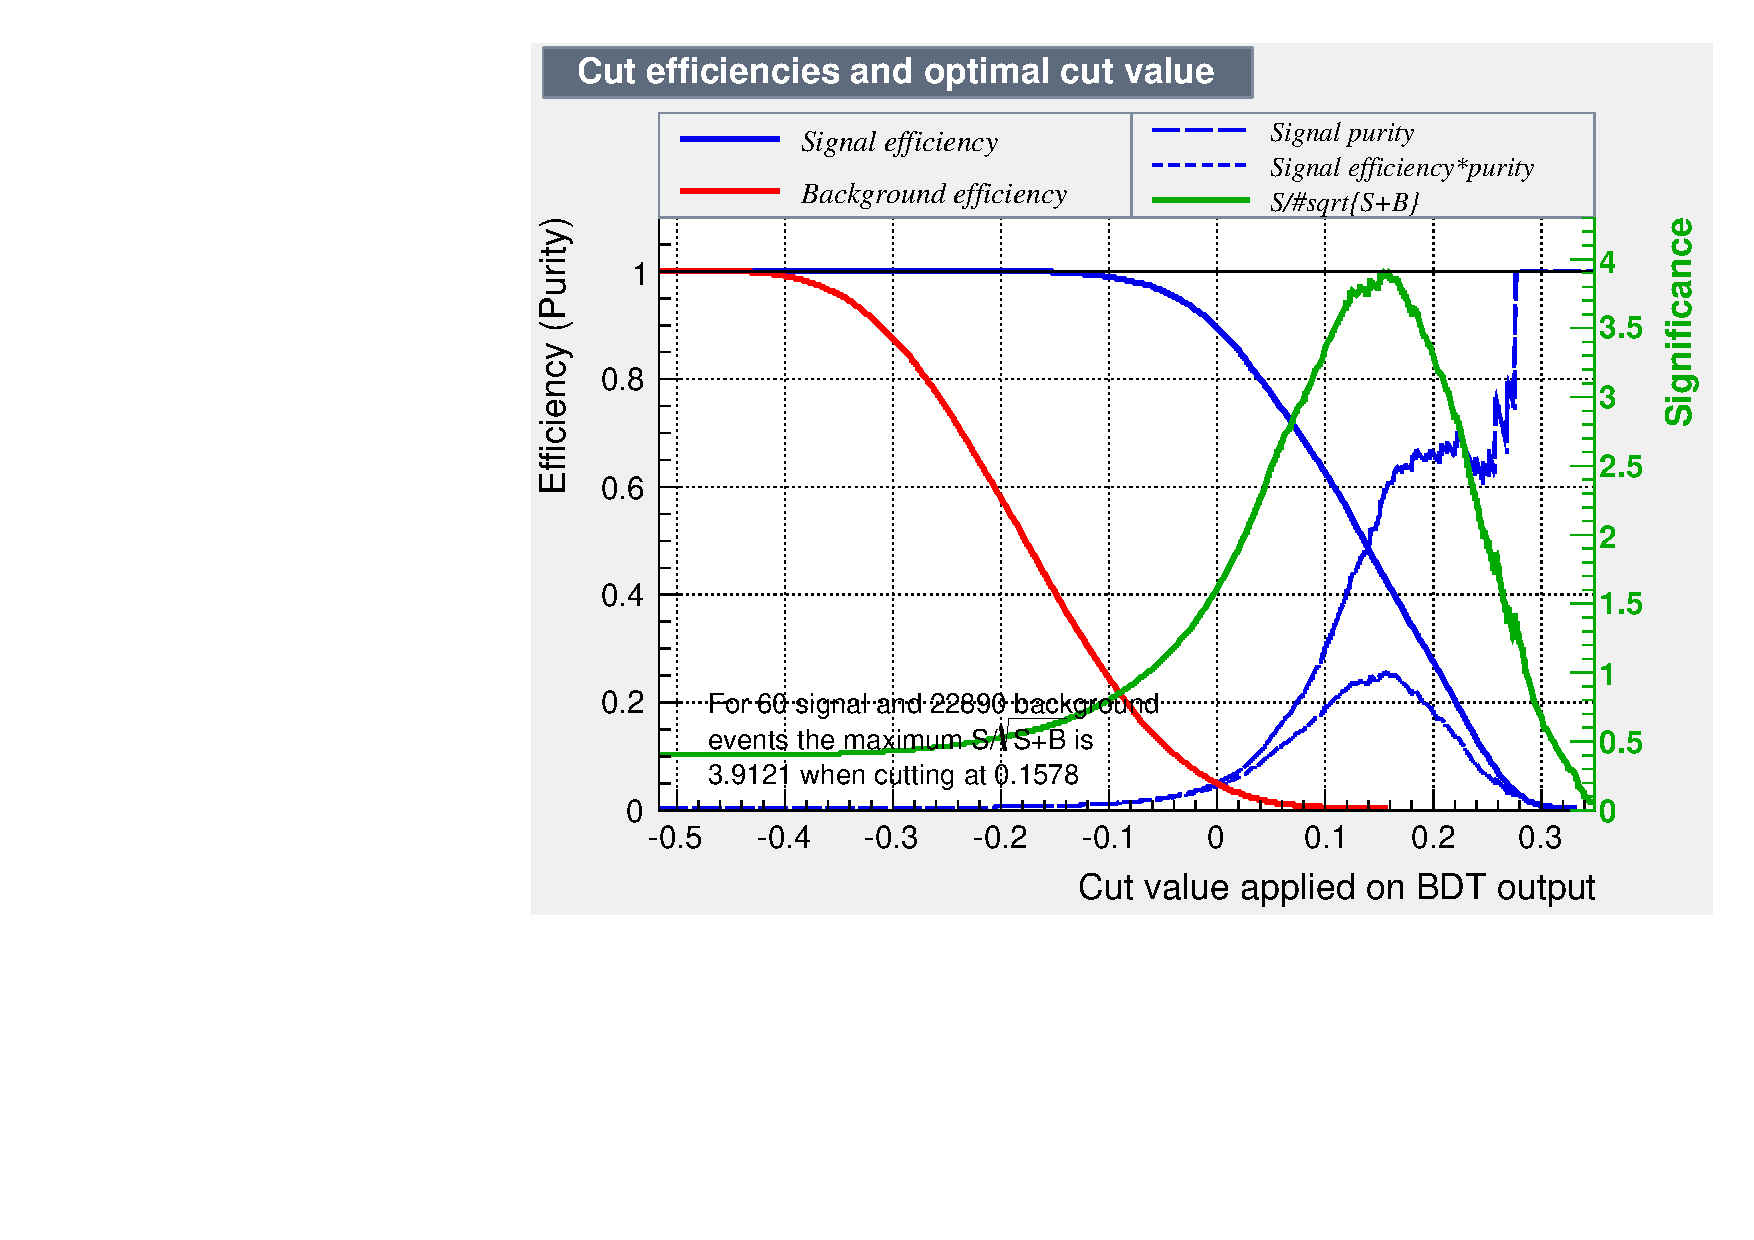
\includegraphics[width=0.45\textwidth]{Figures/mvaeffs_BDT_barrel.pdf}
  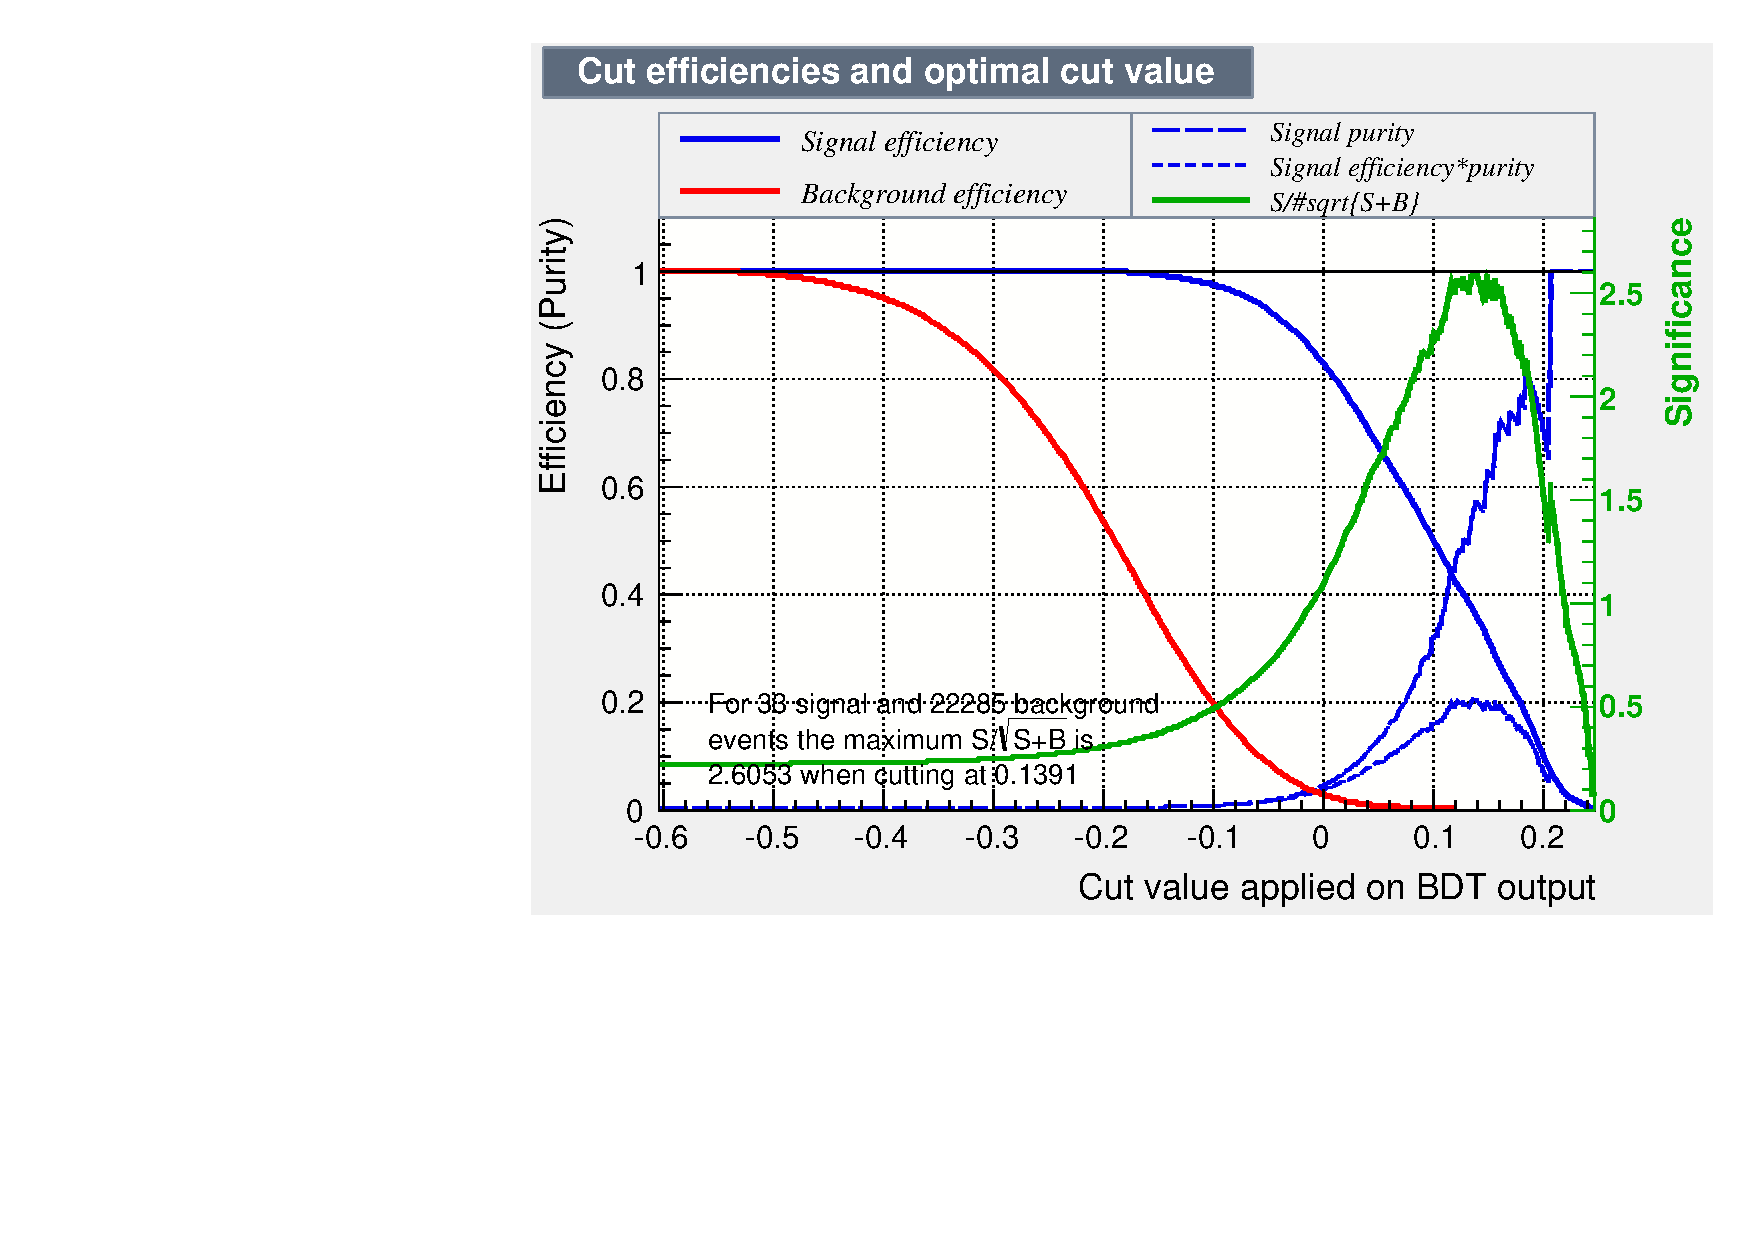
\includegraphics[width=0.45\textwidth]{Figures/mvaeffs_BDT_endcaps.pdf}
  \caption{Optimal BDT cut value for barrel (left) and endcaps (right).}
  \label{fig:massOptimalCut}
\end{figure}

\begin{figure}
  \centering
  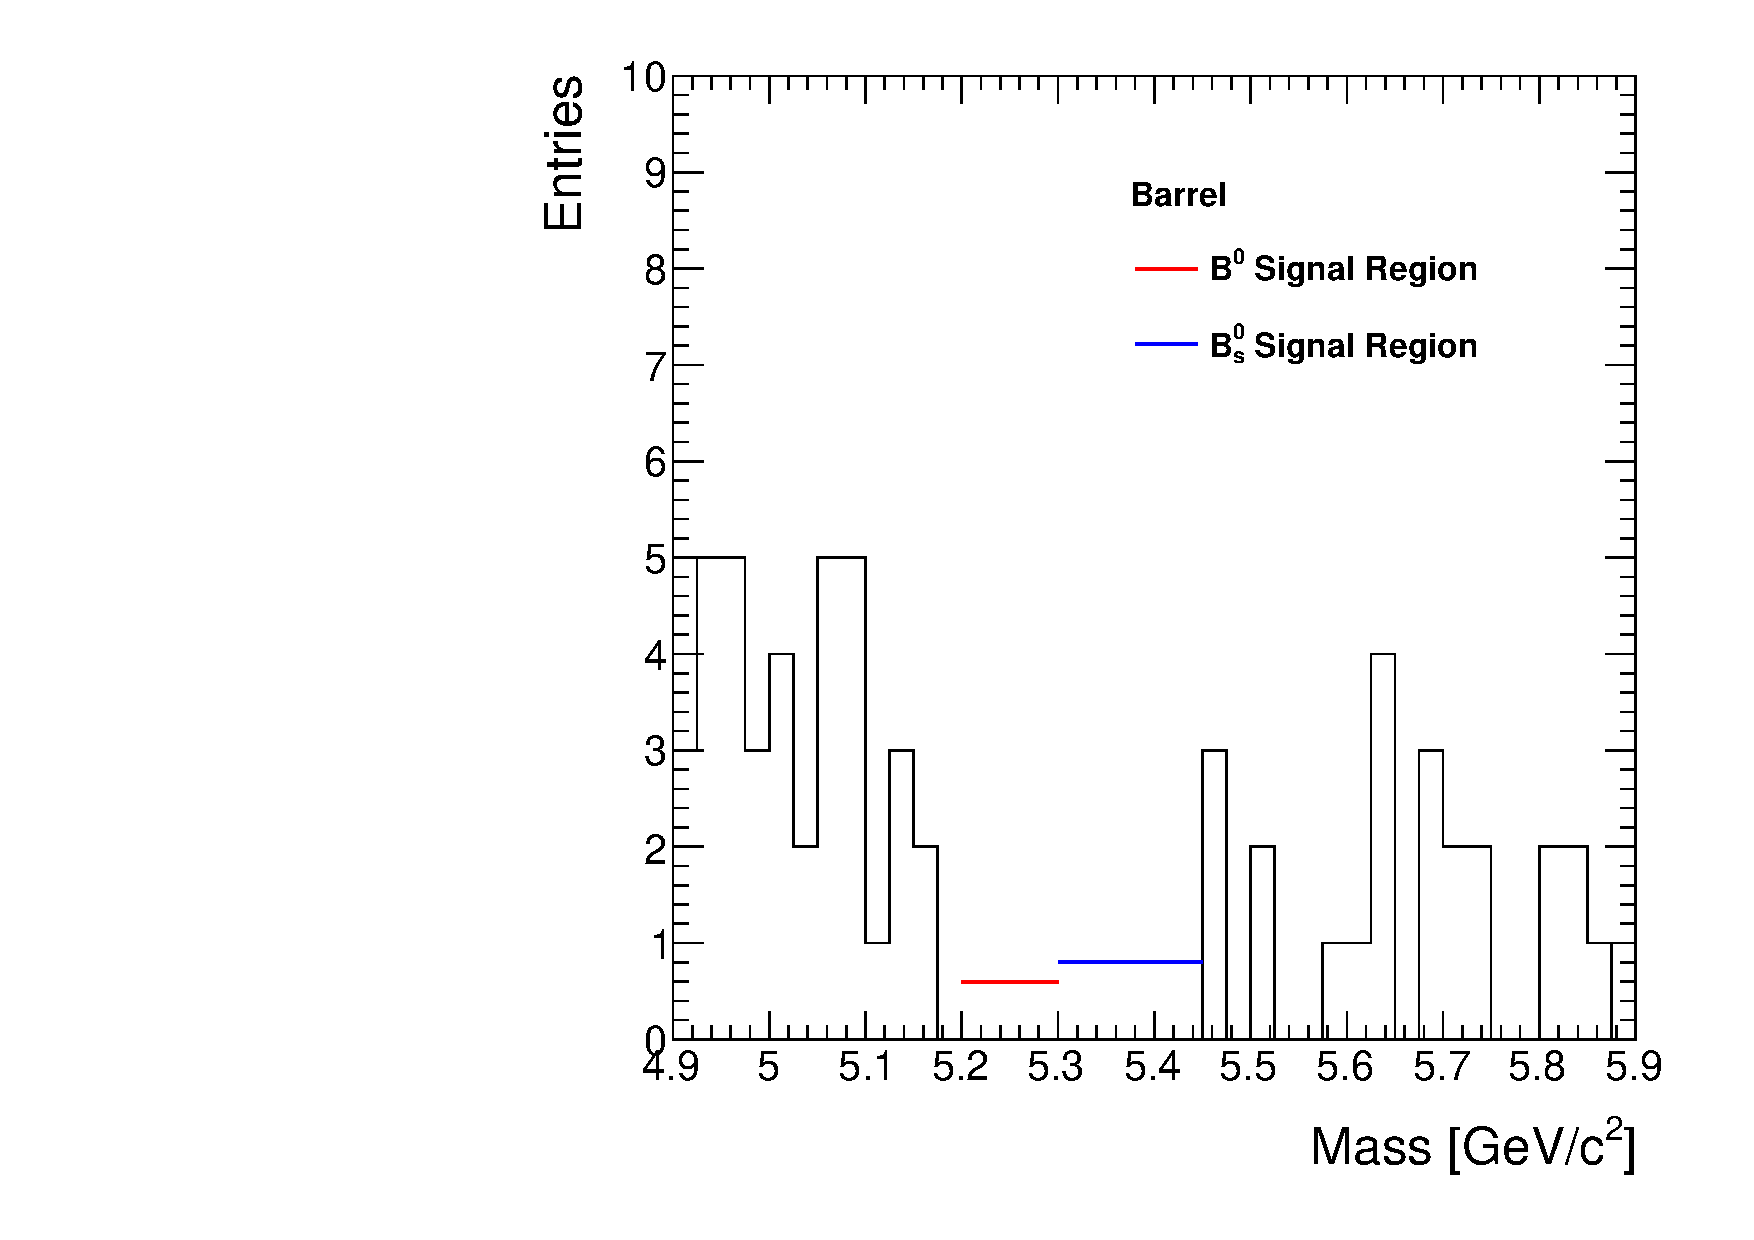
\includegraphics[width=0.45\textwidth]{Figures/BarrelMassPlot.pdf}
  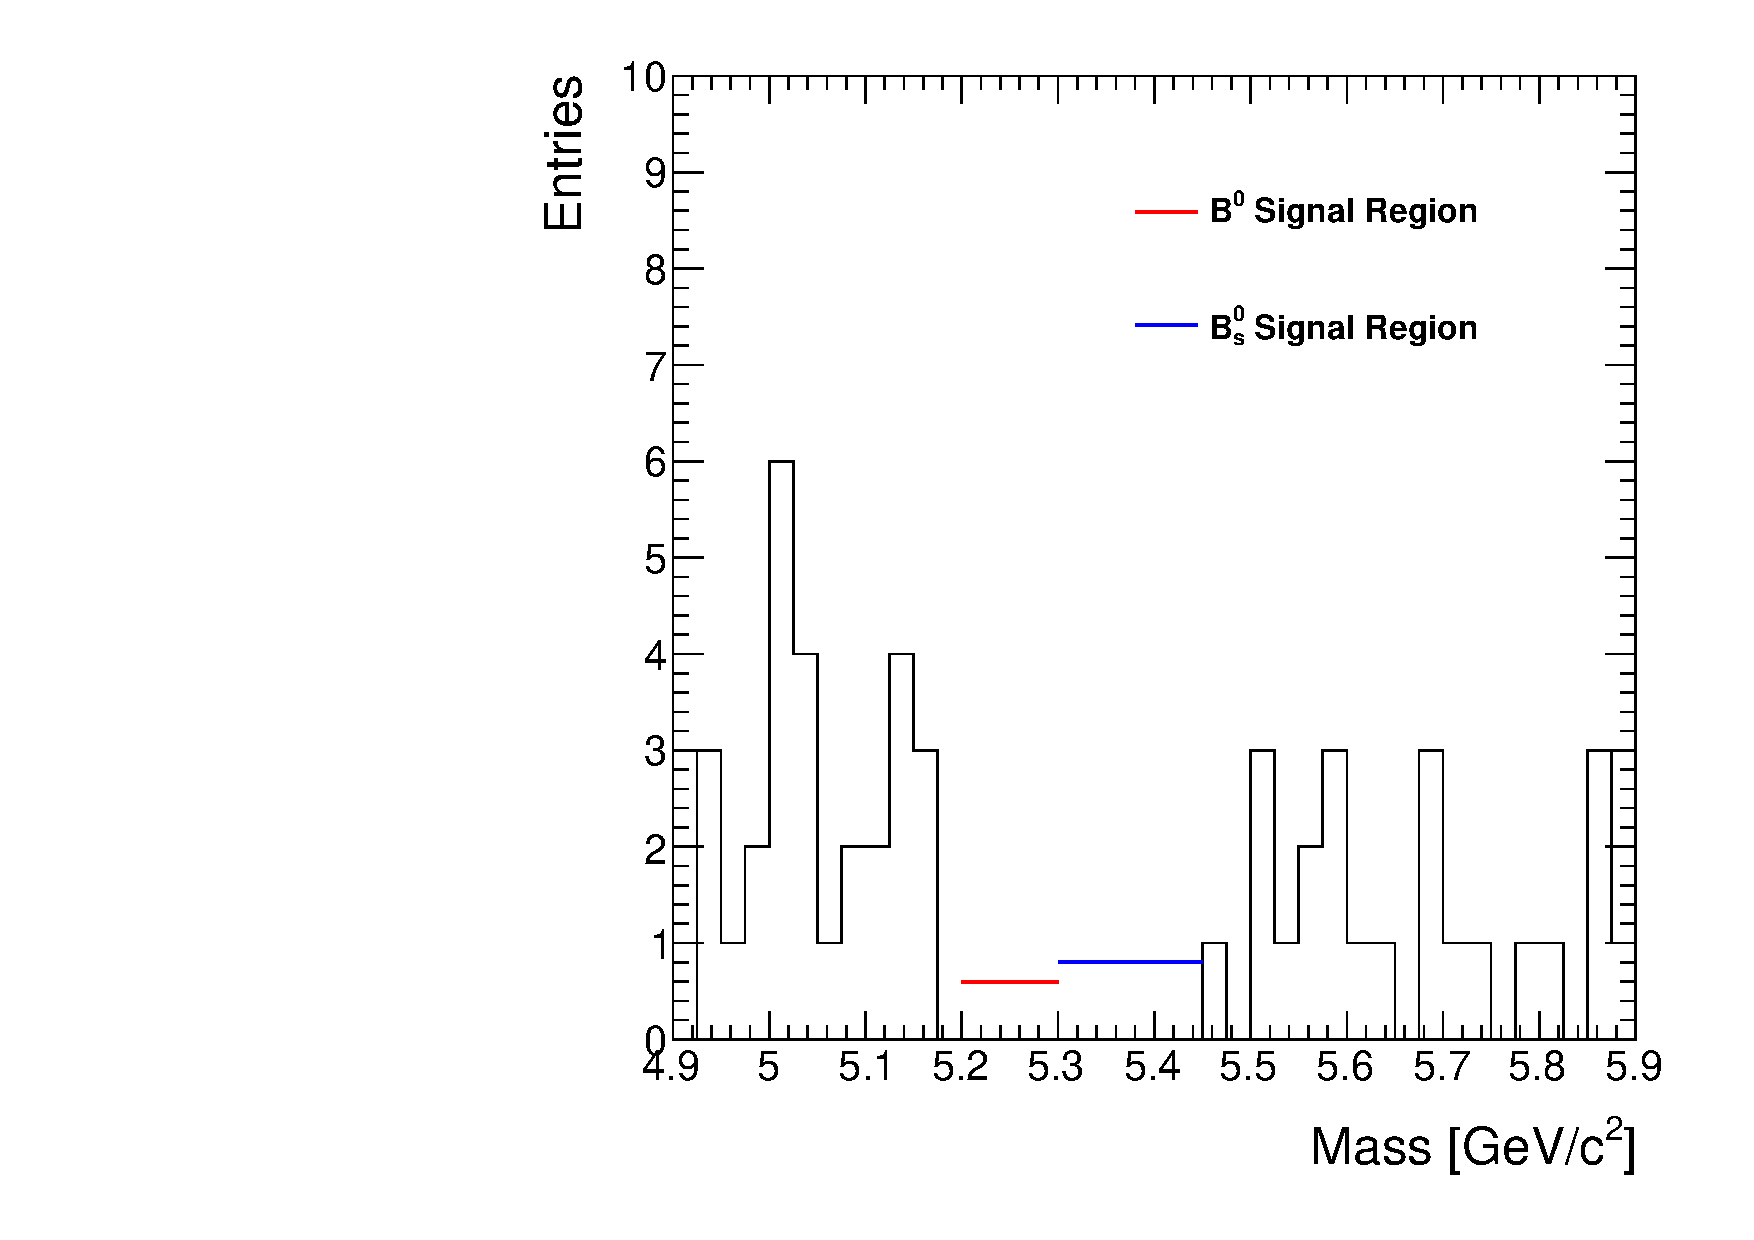
\includegraphics[width=0.45\textwidth]{Figures/EndcapsMassPlot.pdf}
  \caption{Blinded invariant mass distribution for all candidates passing the BDT selection for barrel (left) and endcaps (right).}
  \label{fig:massPlotBlinded}
\end{figure}

Figures \ref{fig:massPlotUnblinded} shows the unblinded invariant mass distribution after applying the BDT selection.

\begin{figure}
  \centering
  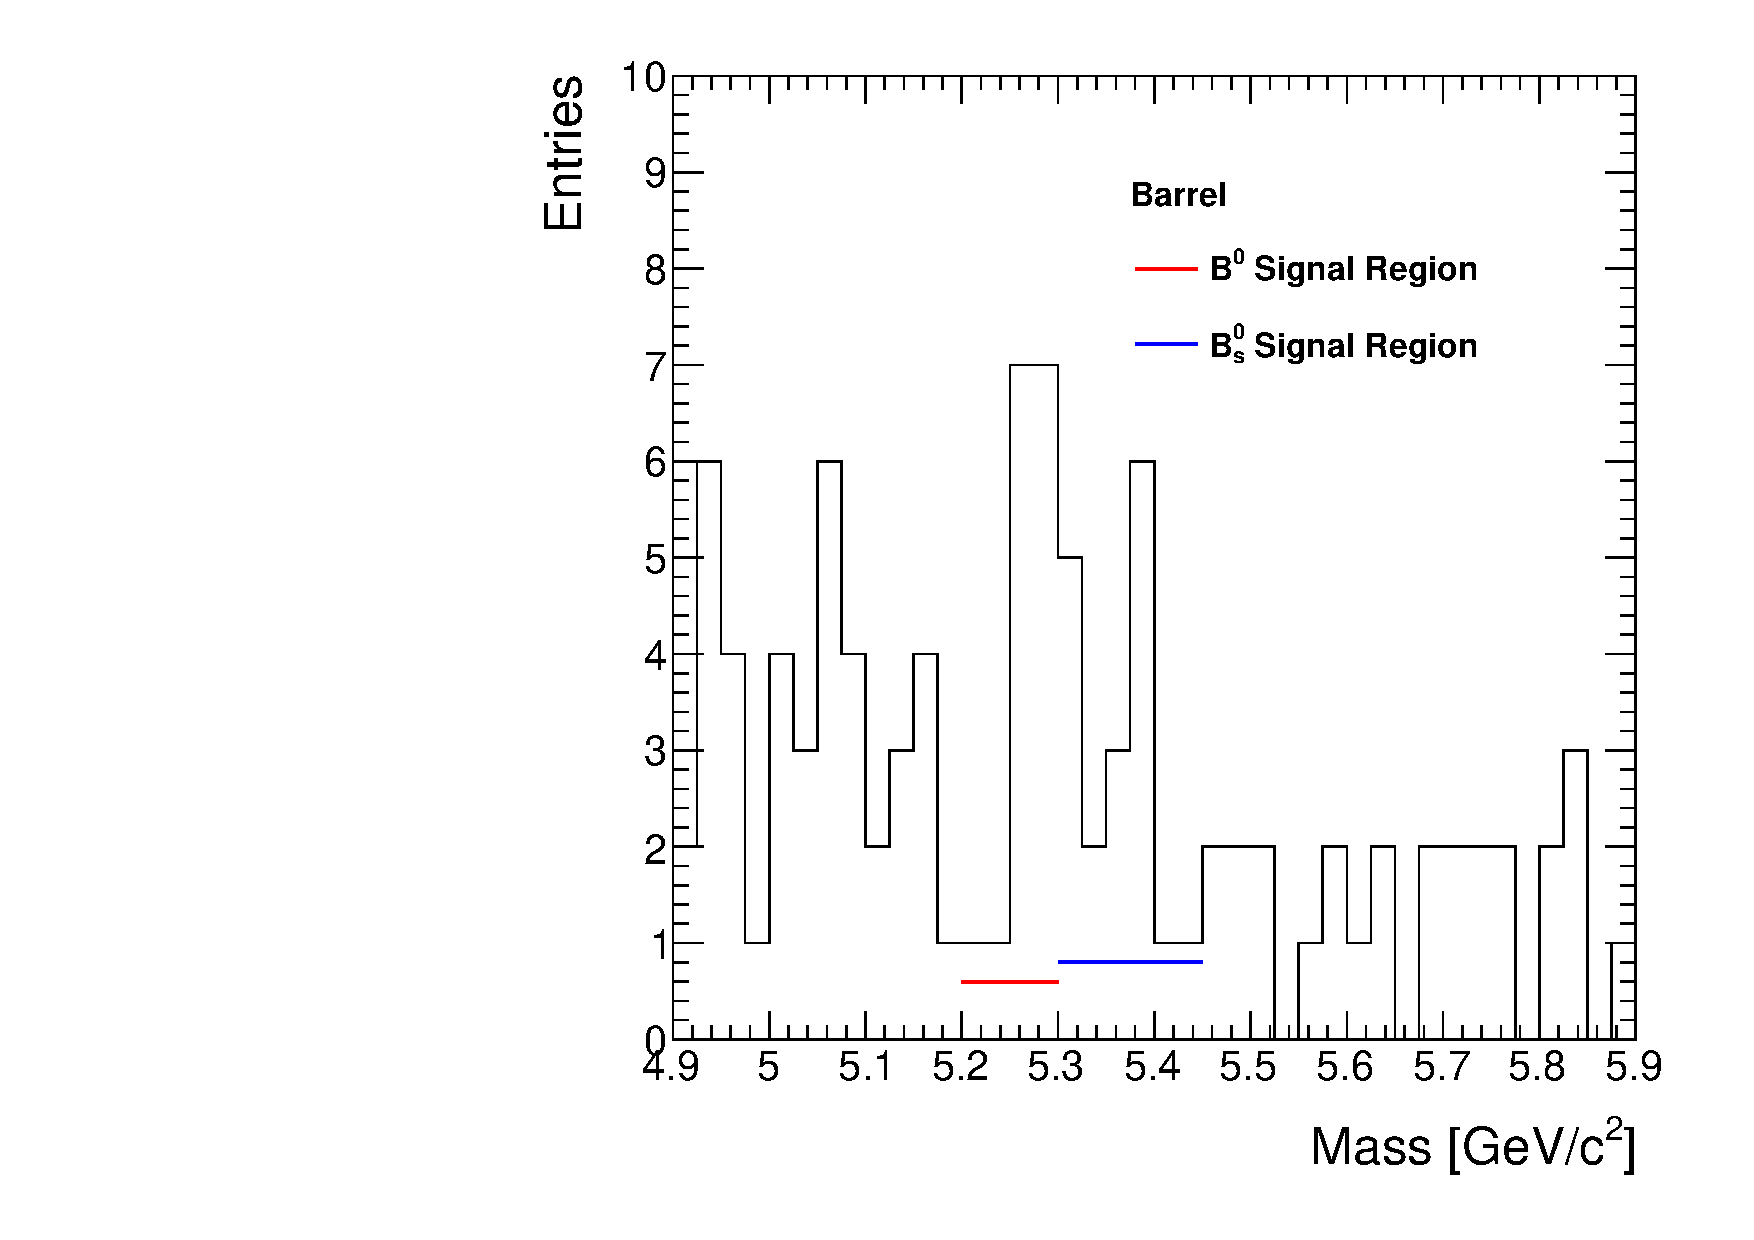
\includegraphics[width=0.45\textwidth]{Figures/BarrelMassPlotUnblinded.pdf}
  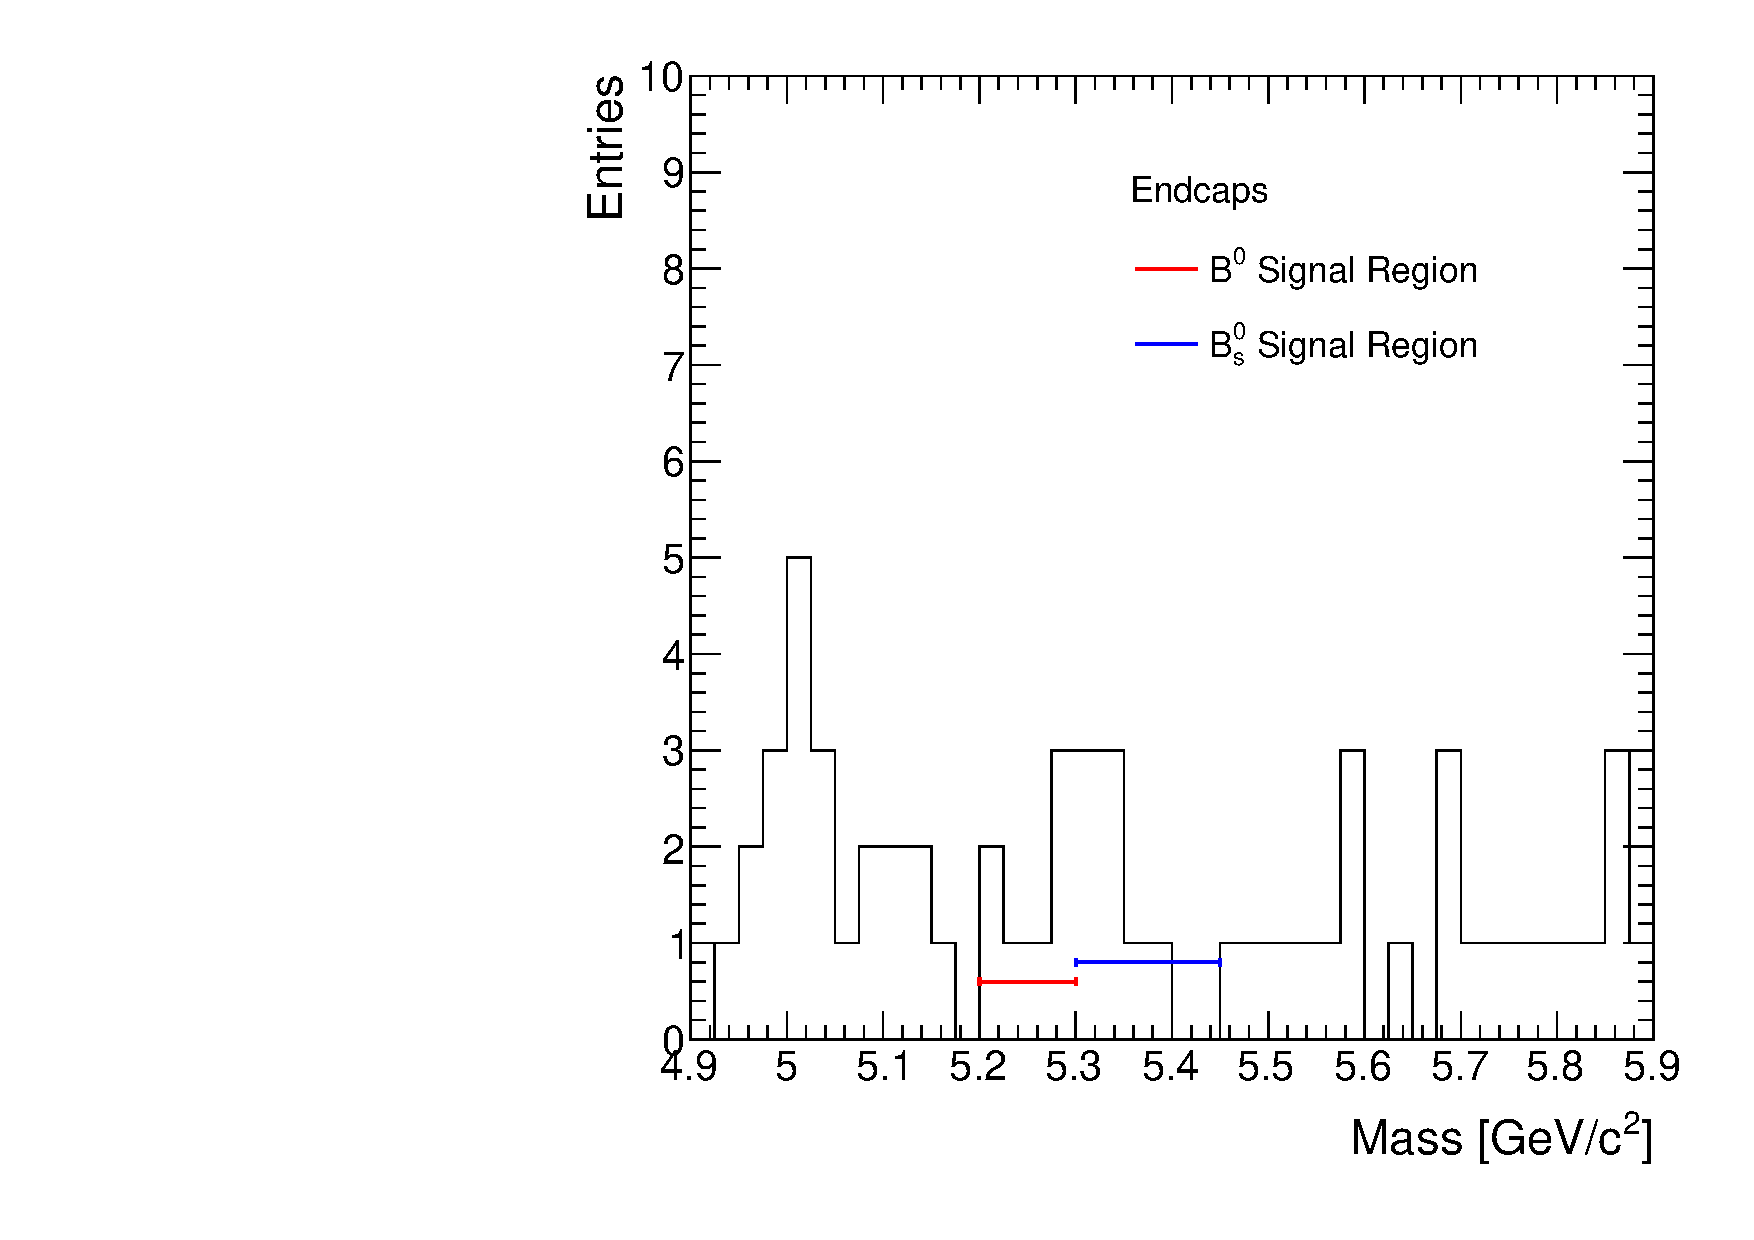
\includegraphics[width=0.45\textwidth]{Figures/EndcapsMassPlotUnblinded.pdf}
  \caption{Unblinded invariant mass distribution for all candidates passing the BDT selection for barrel (left) and endcaps (right).}
  \label{fig:massPlotUnblinded}
\end{figure}


Figures \ref{fig:AfterBDTCutVariablesBarrelBlinded}, \ref{fig:AfterBDTCutVariablesEndcapsBlinded}, \ref{fig:AfterBDTCutVariablesBarrelUnblinded} and \ref{fig:AfterBDTCutVariablesEndcapsUnblinded} show variable distributions after the application of the BDT selection.

\begin{figure}
  \centering
  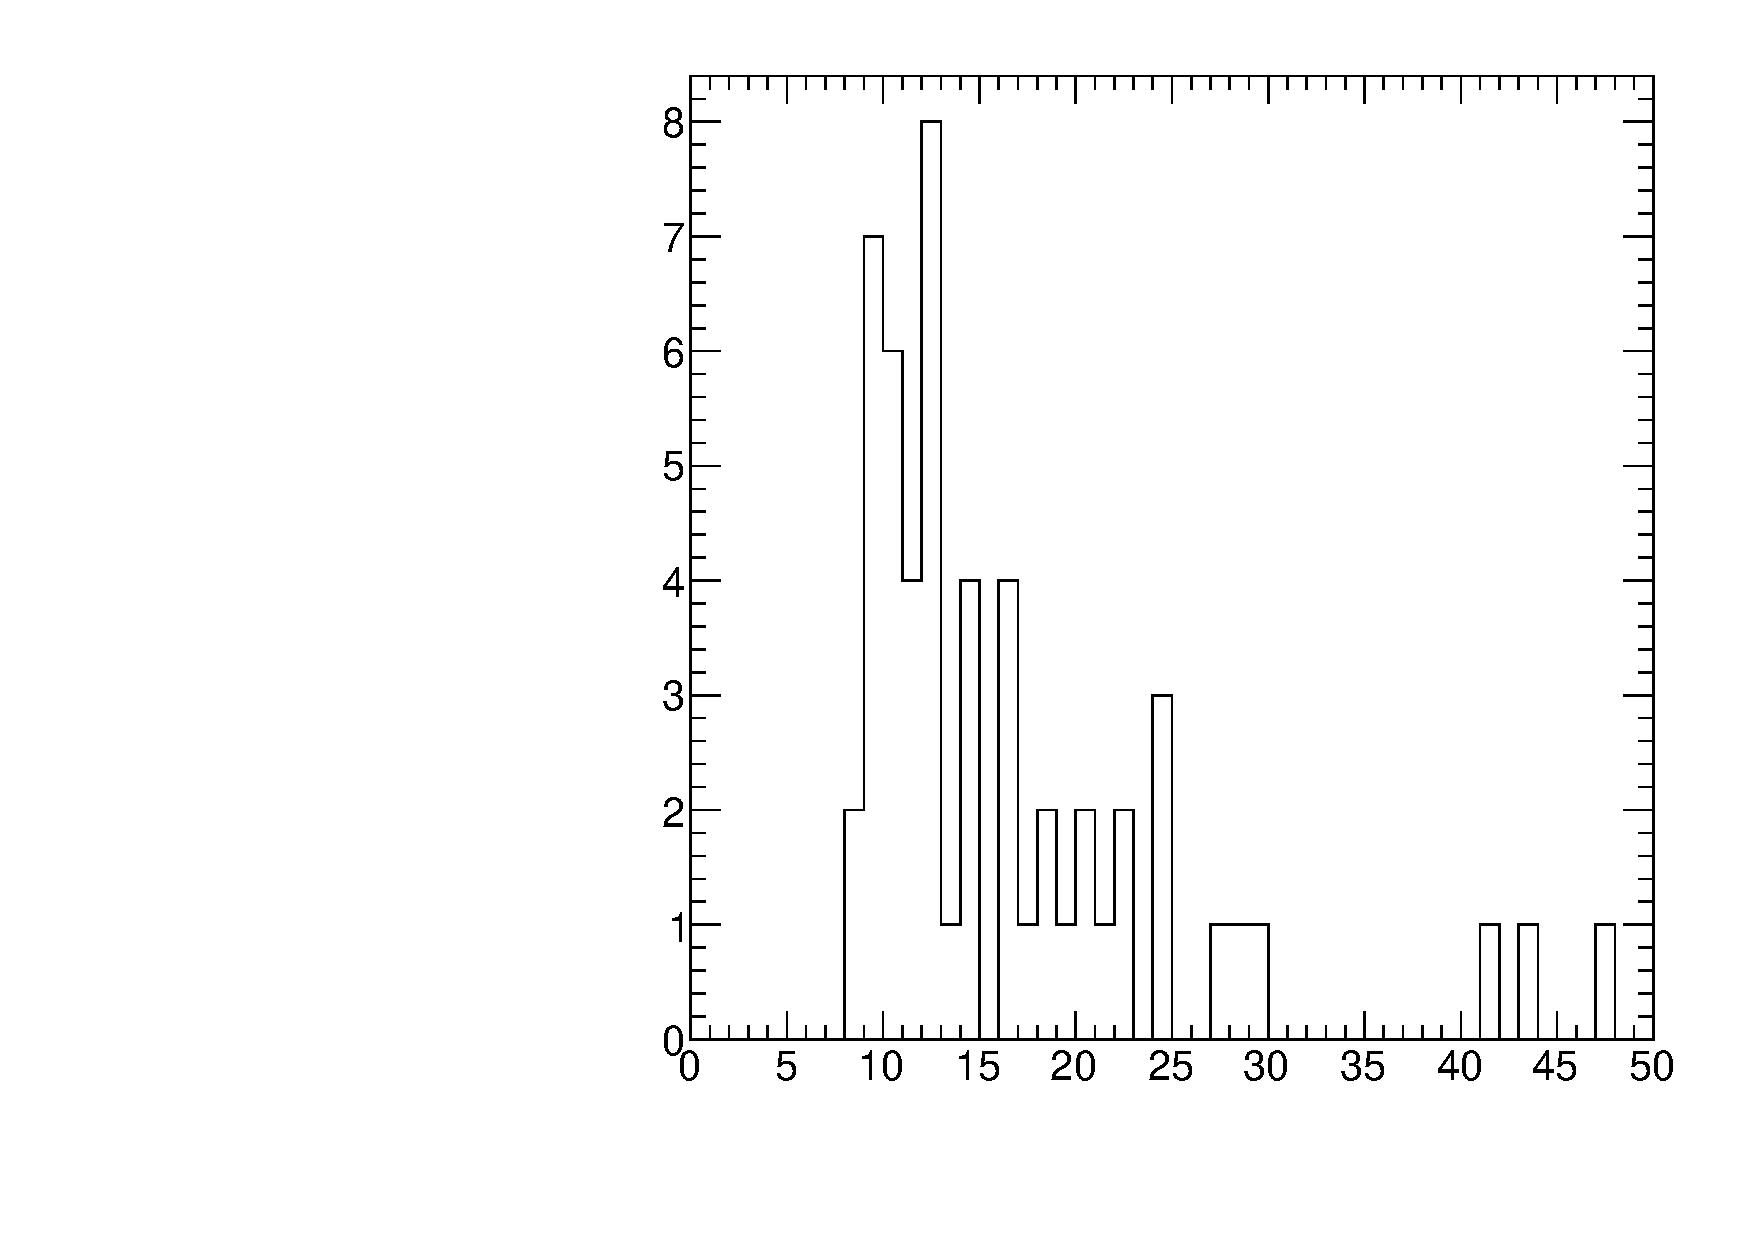
\includegraphics[width=0.3\textwidth]{Figures/AfterBDTCut_pt_Barrel.pdf}
  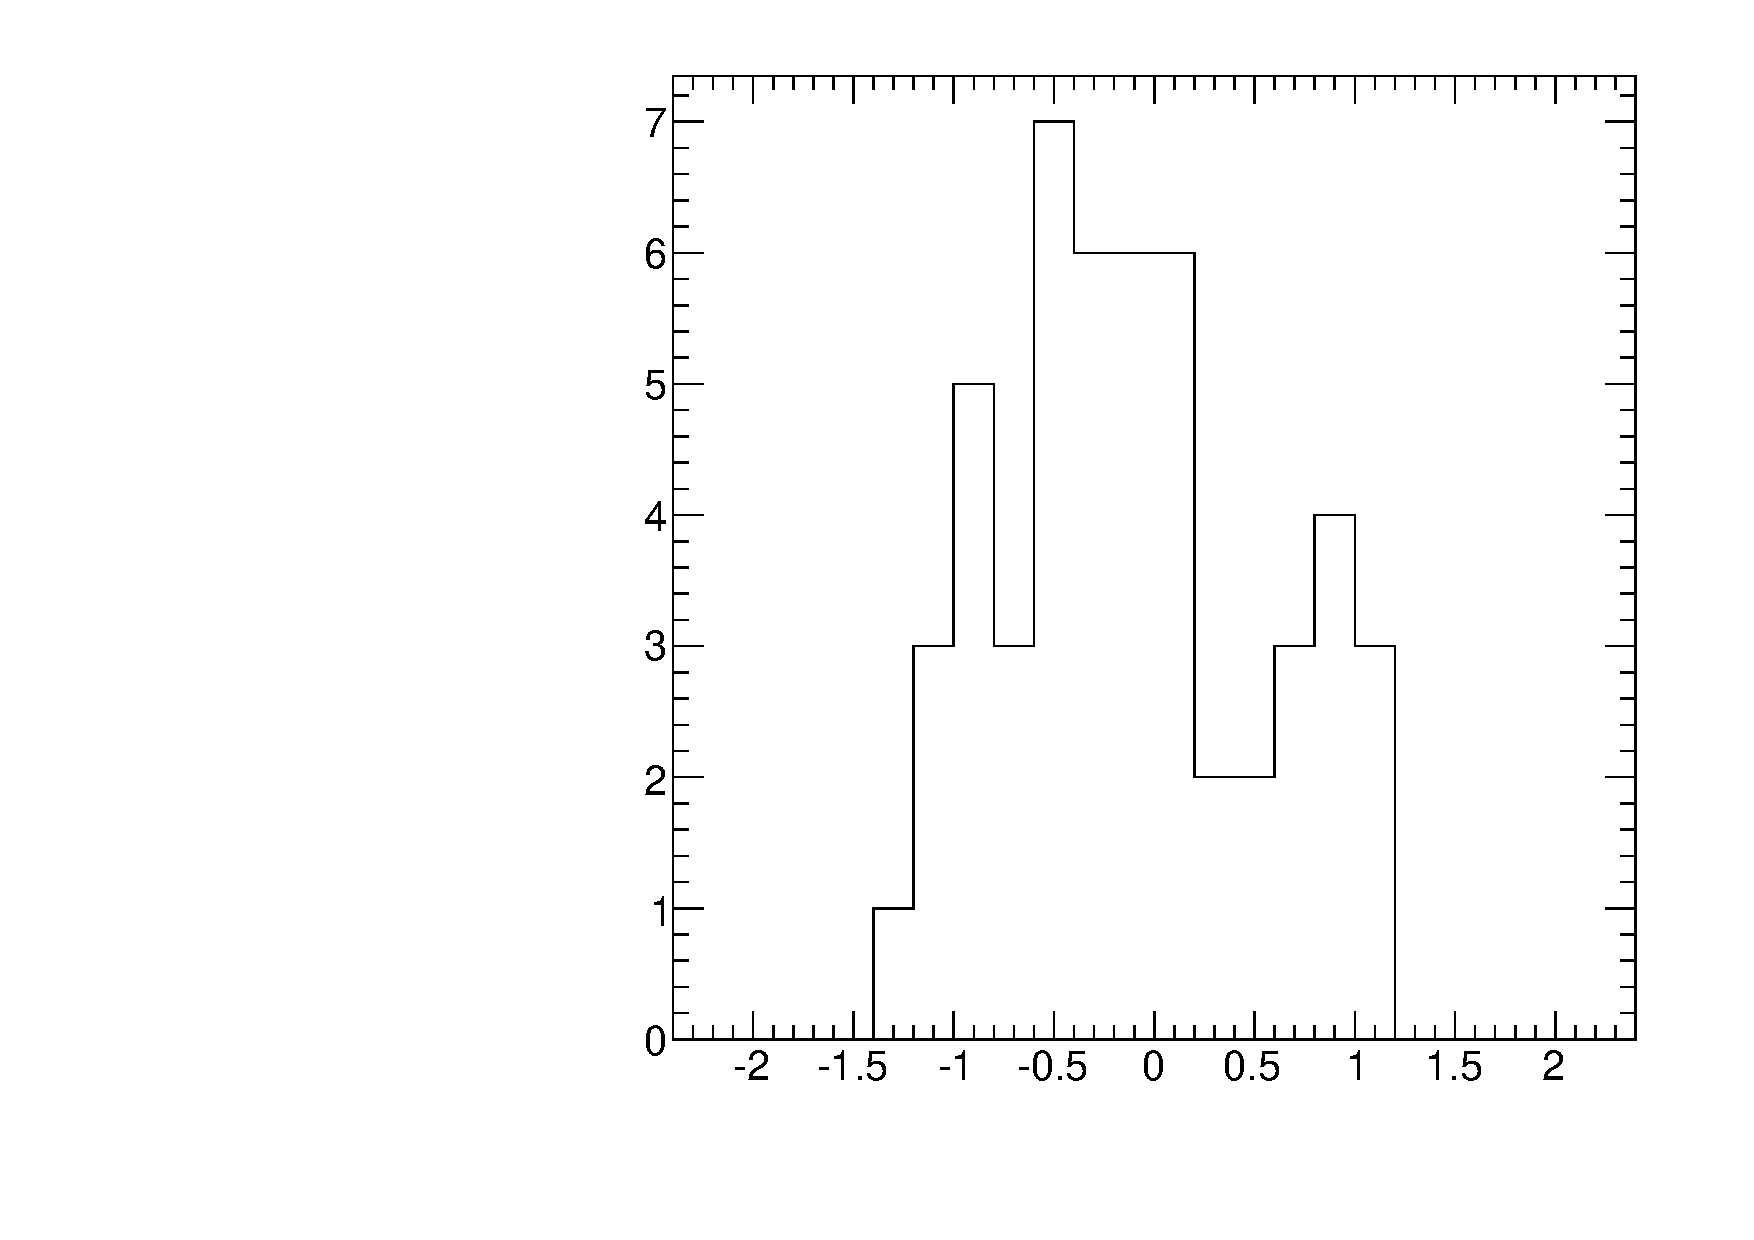
\includegraphics[width=0.3\textwidth]{Figures/AfterBDTCut_eta_Barrel.pdf}
  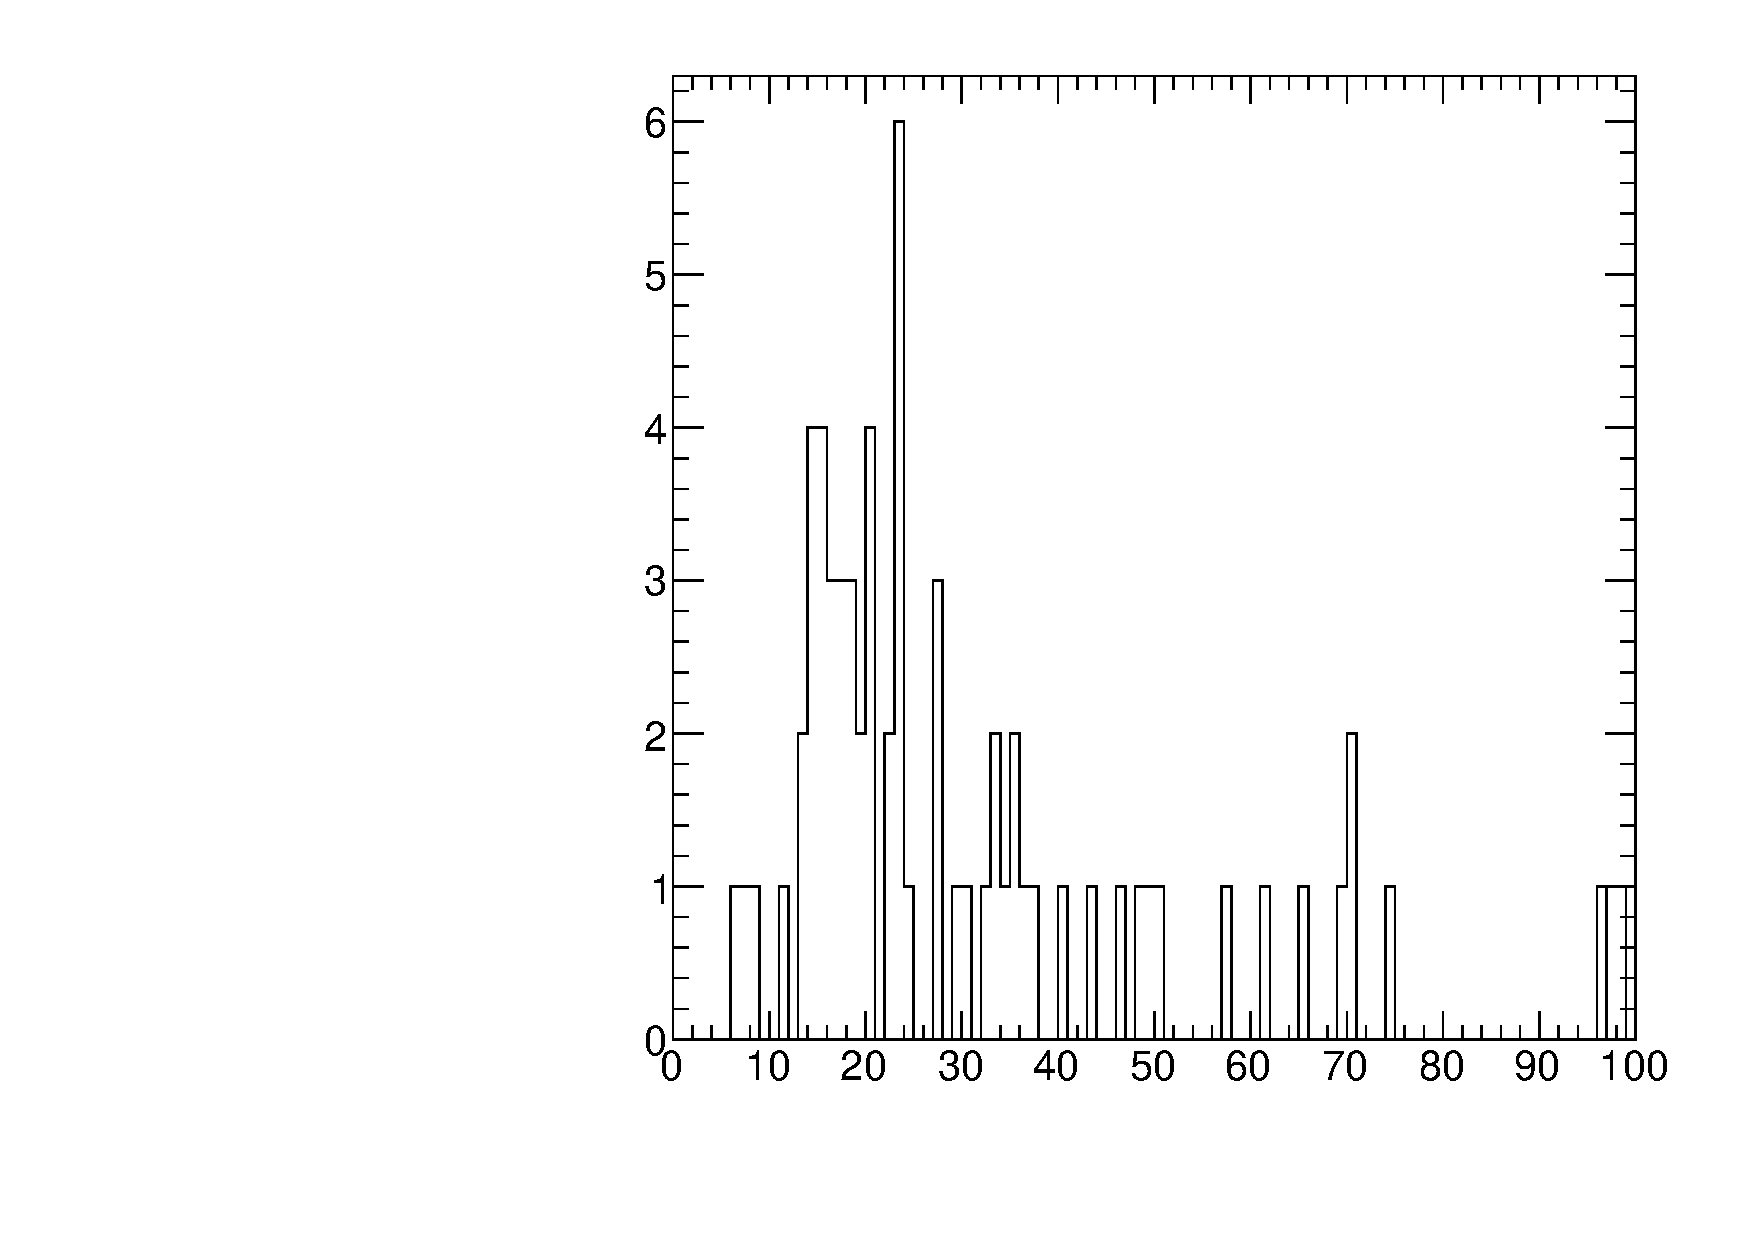
\includegraphics[width=0.3\textwidth]{Figures/AfterBDTCut_fls3d_Barrel.pdf}
  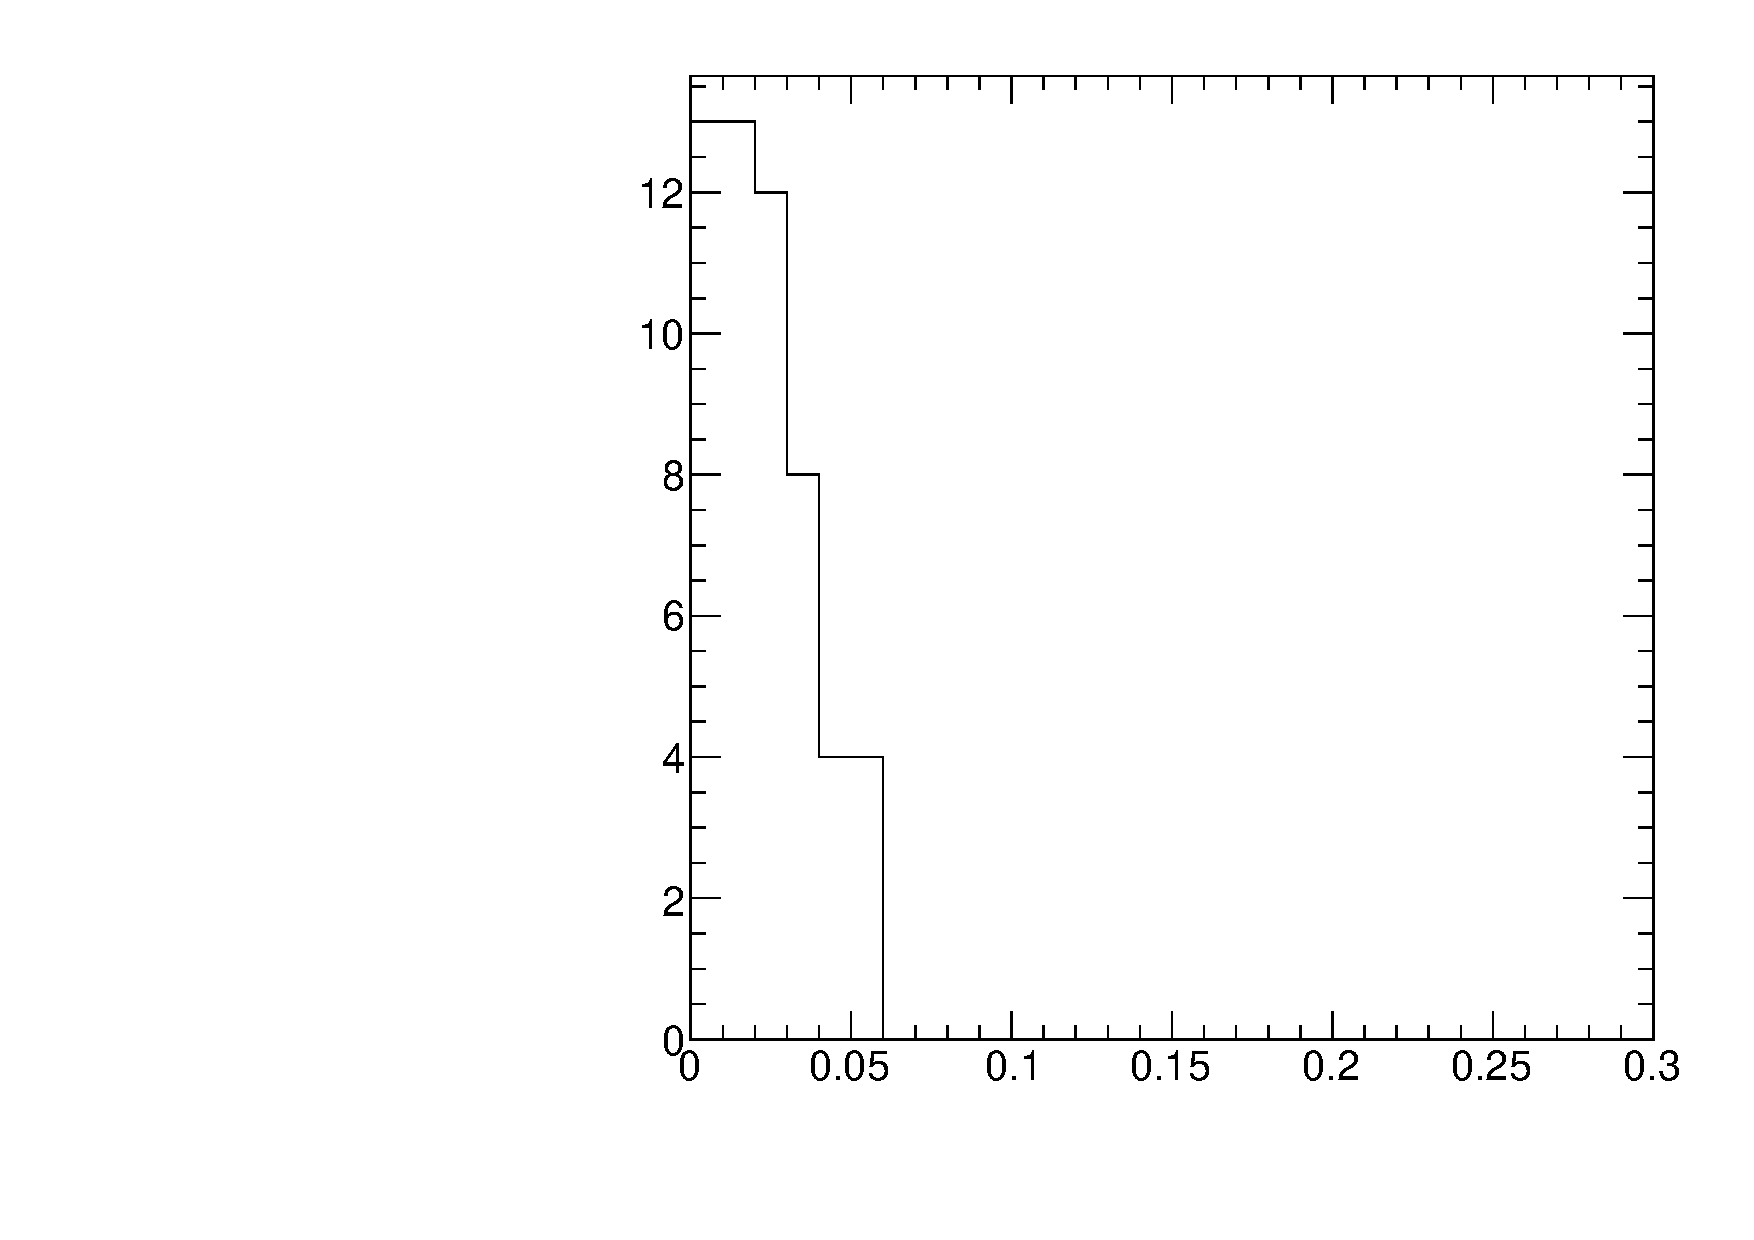
\includegraphics[width=0.3\textwidth]{Figures/AfterBDTCut_alpha_Barrel.pdf}
  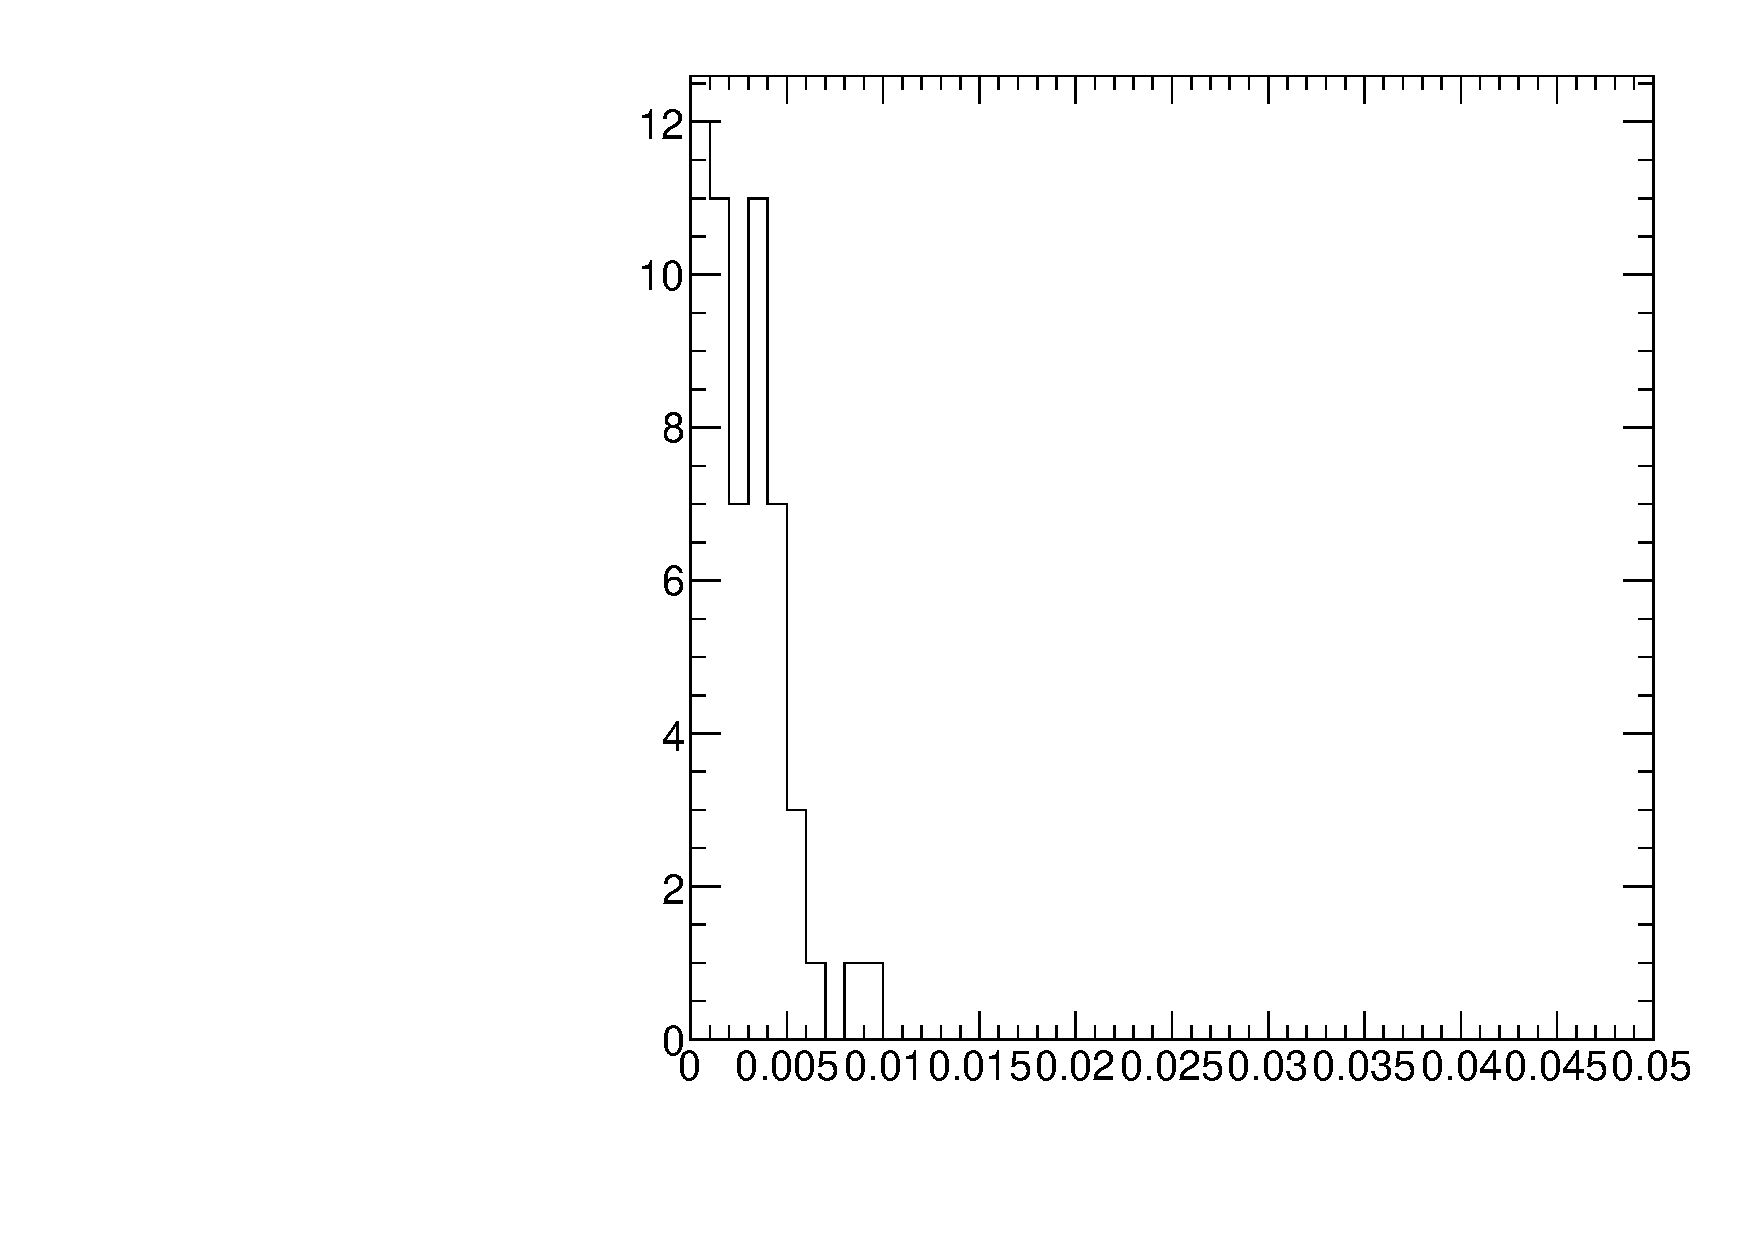
\includegraphics[width=0.3\textwidth]{Figures/AfterBDTCut_maxdoca_Barrel.pdf}
  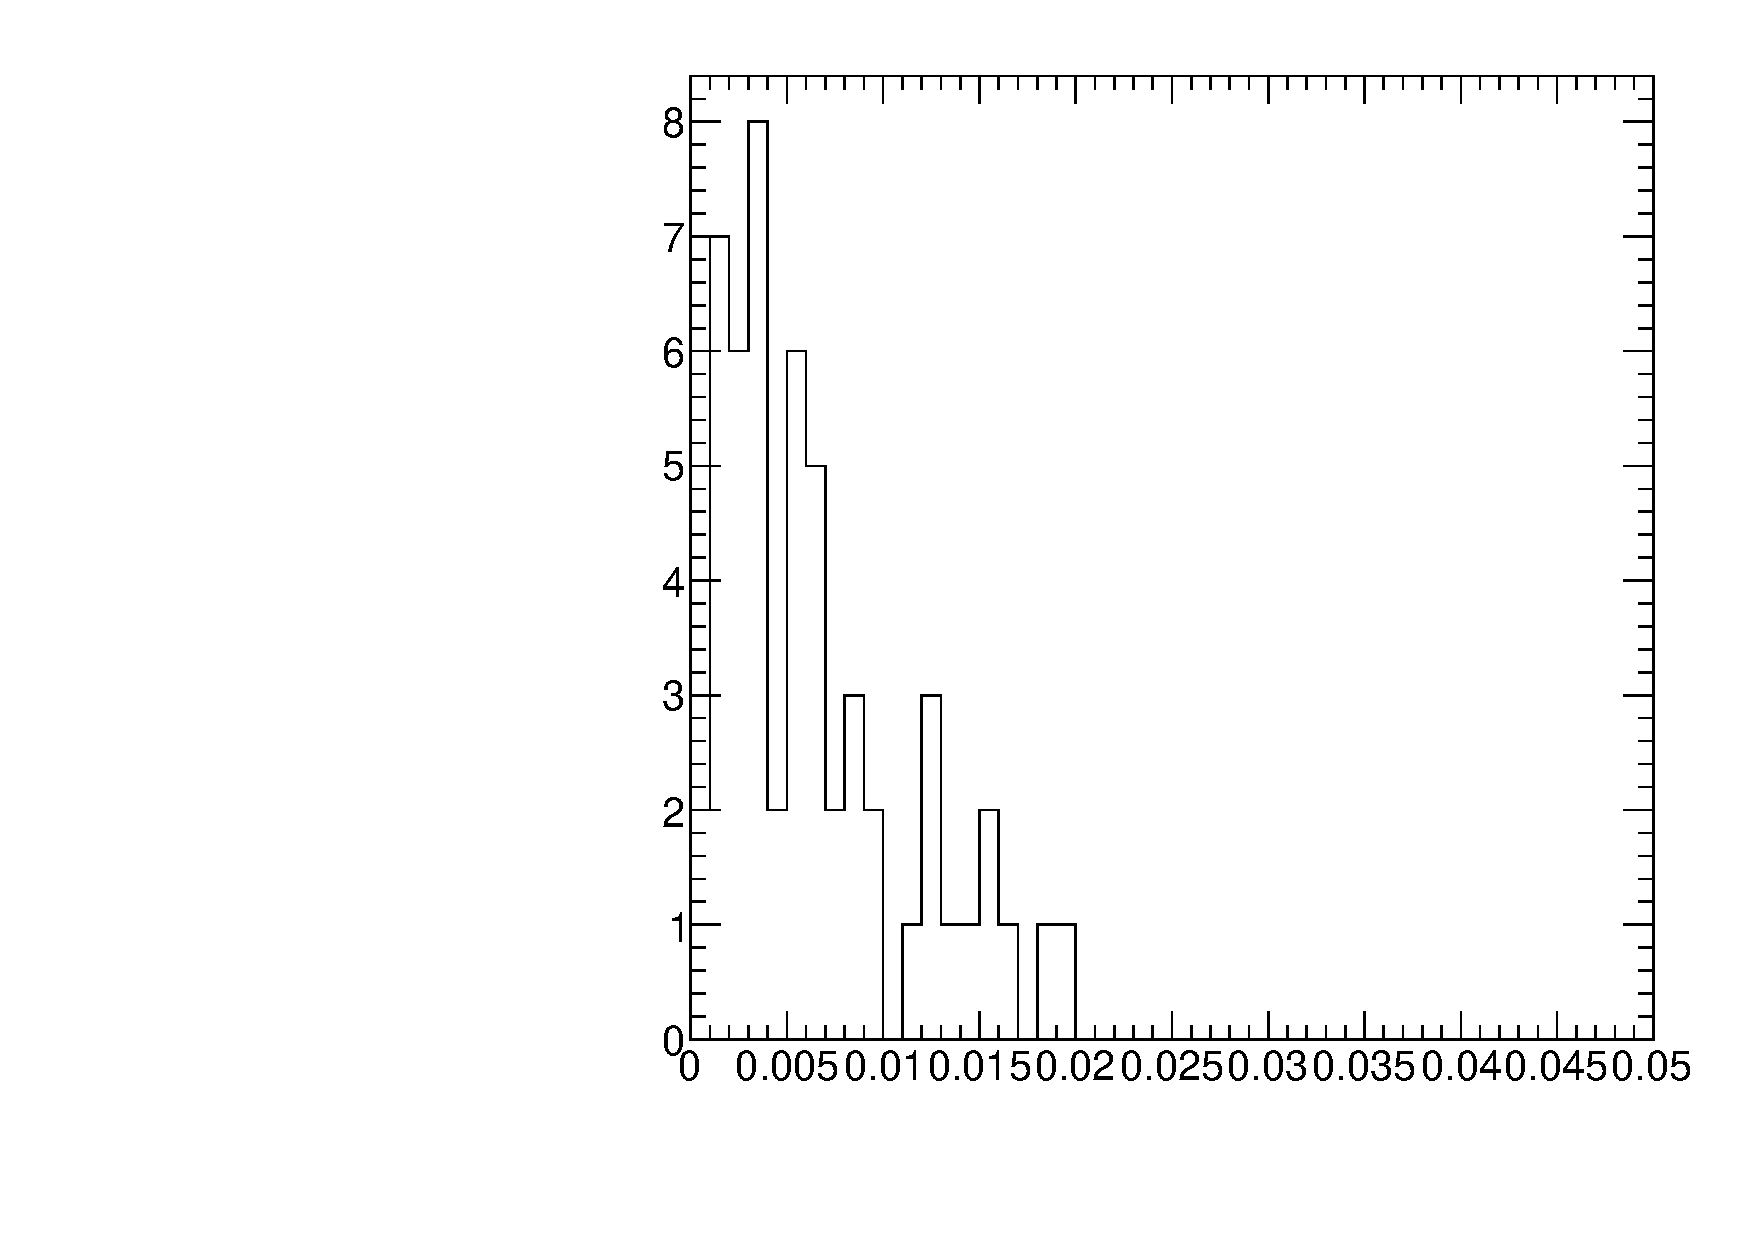
\includegraphics[width=0.3\textwidth]{Figures/AfterBDTCut_pvip_Barrel.pdf}
  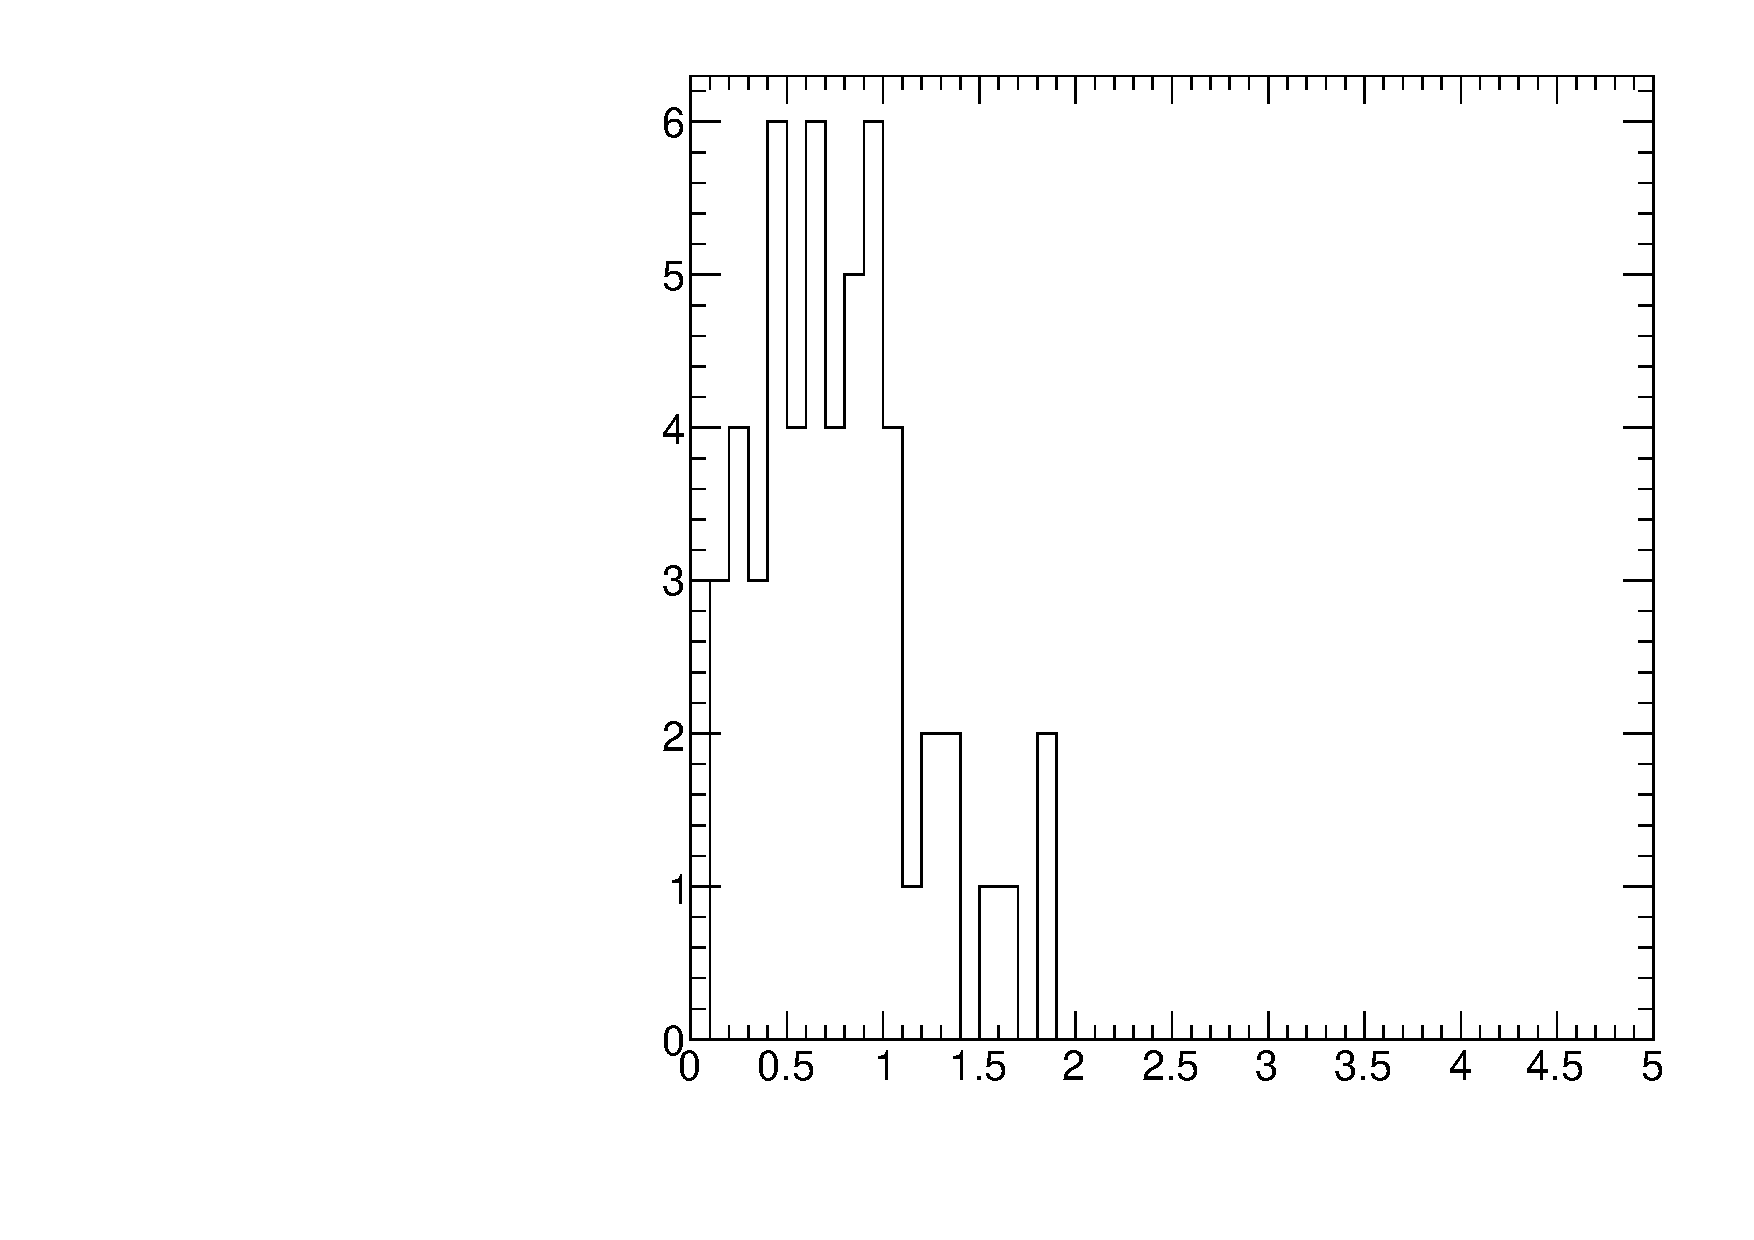
\includegraphics[width=0.3\textwidth]{Figures/AfterBDTCut_pvips_Barrel.pdf}
  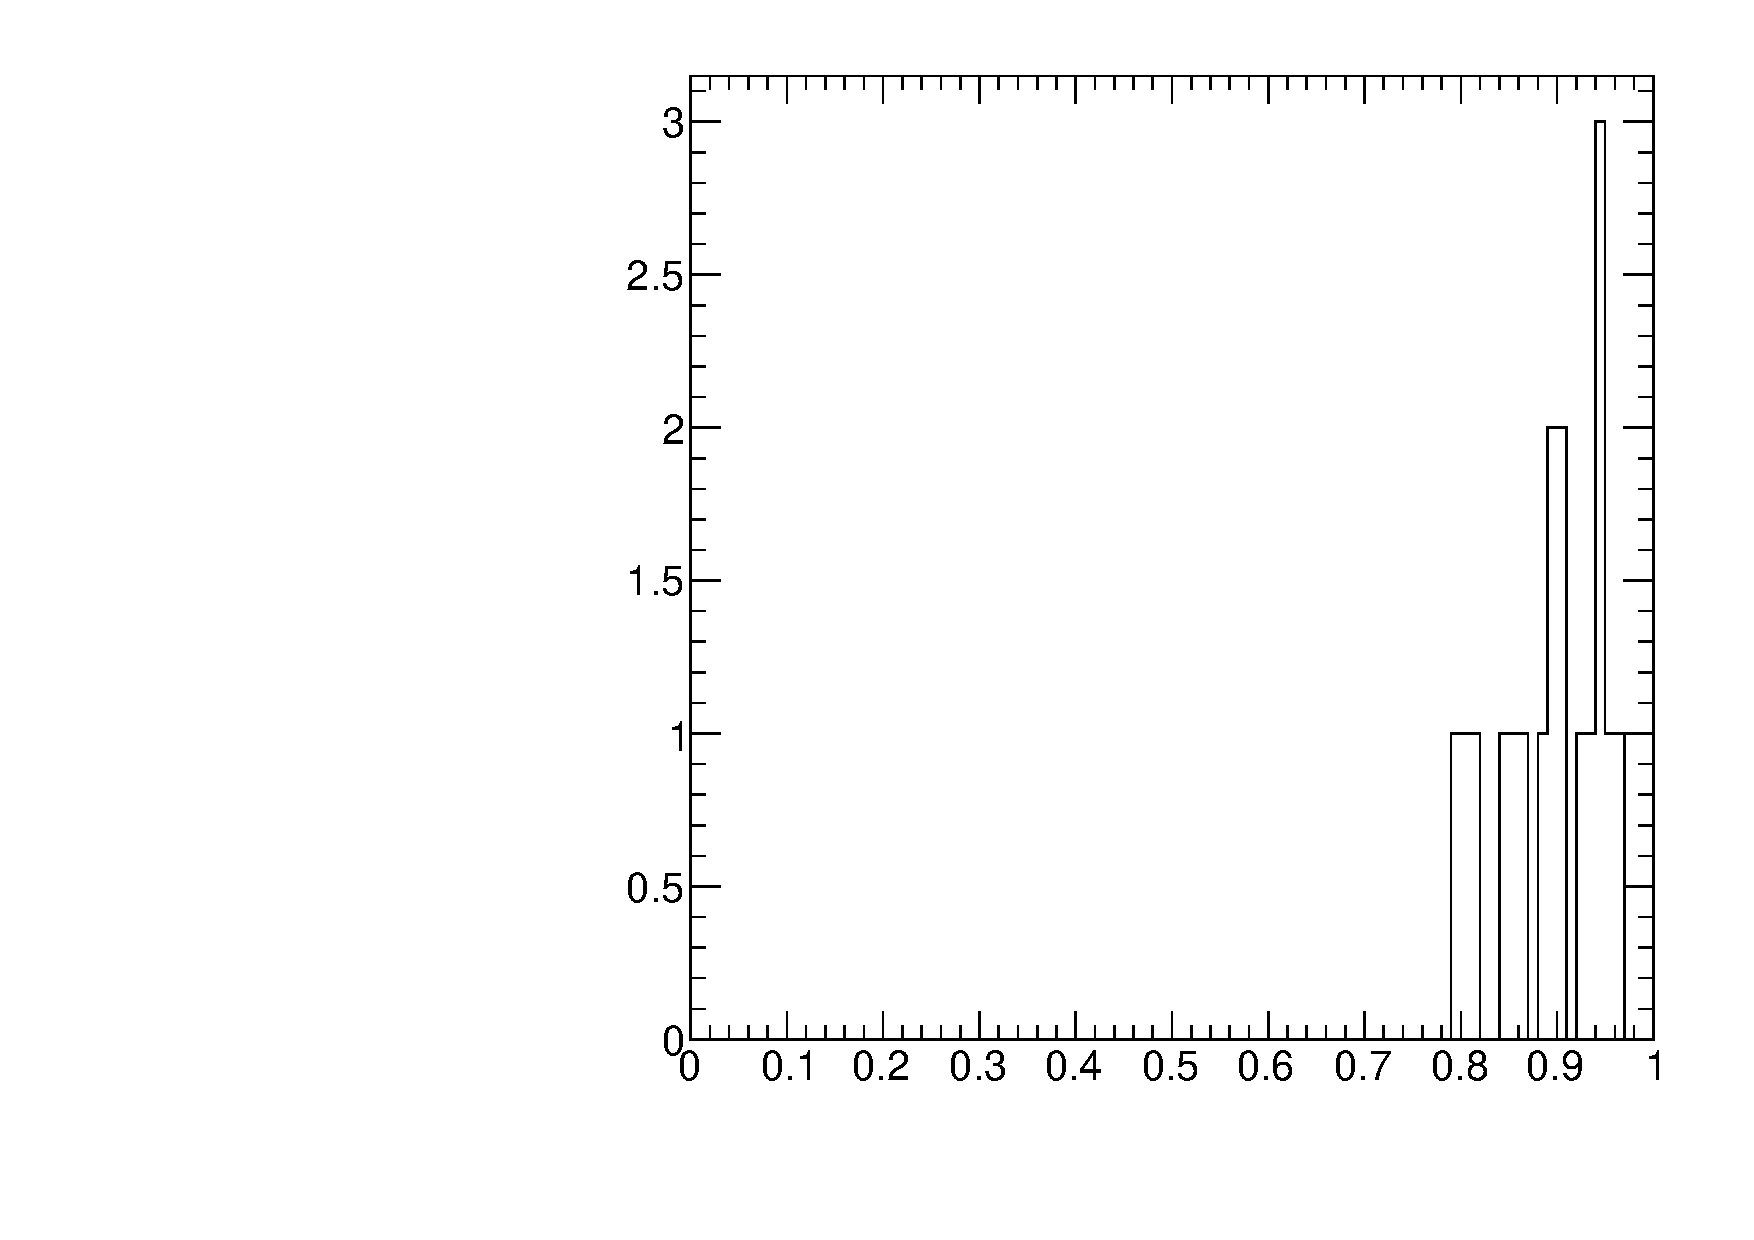
\includegraphics[width=0.3\textwidth]{Figures/AfterBDTCut_iso_Barrel.pdf}
  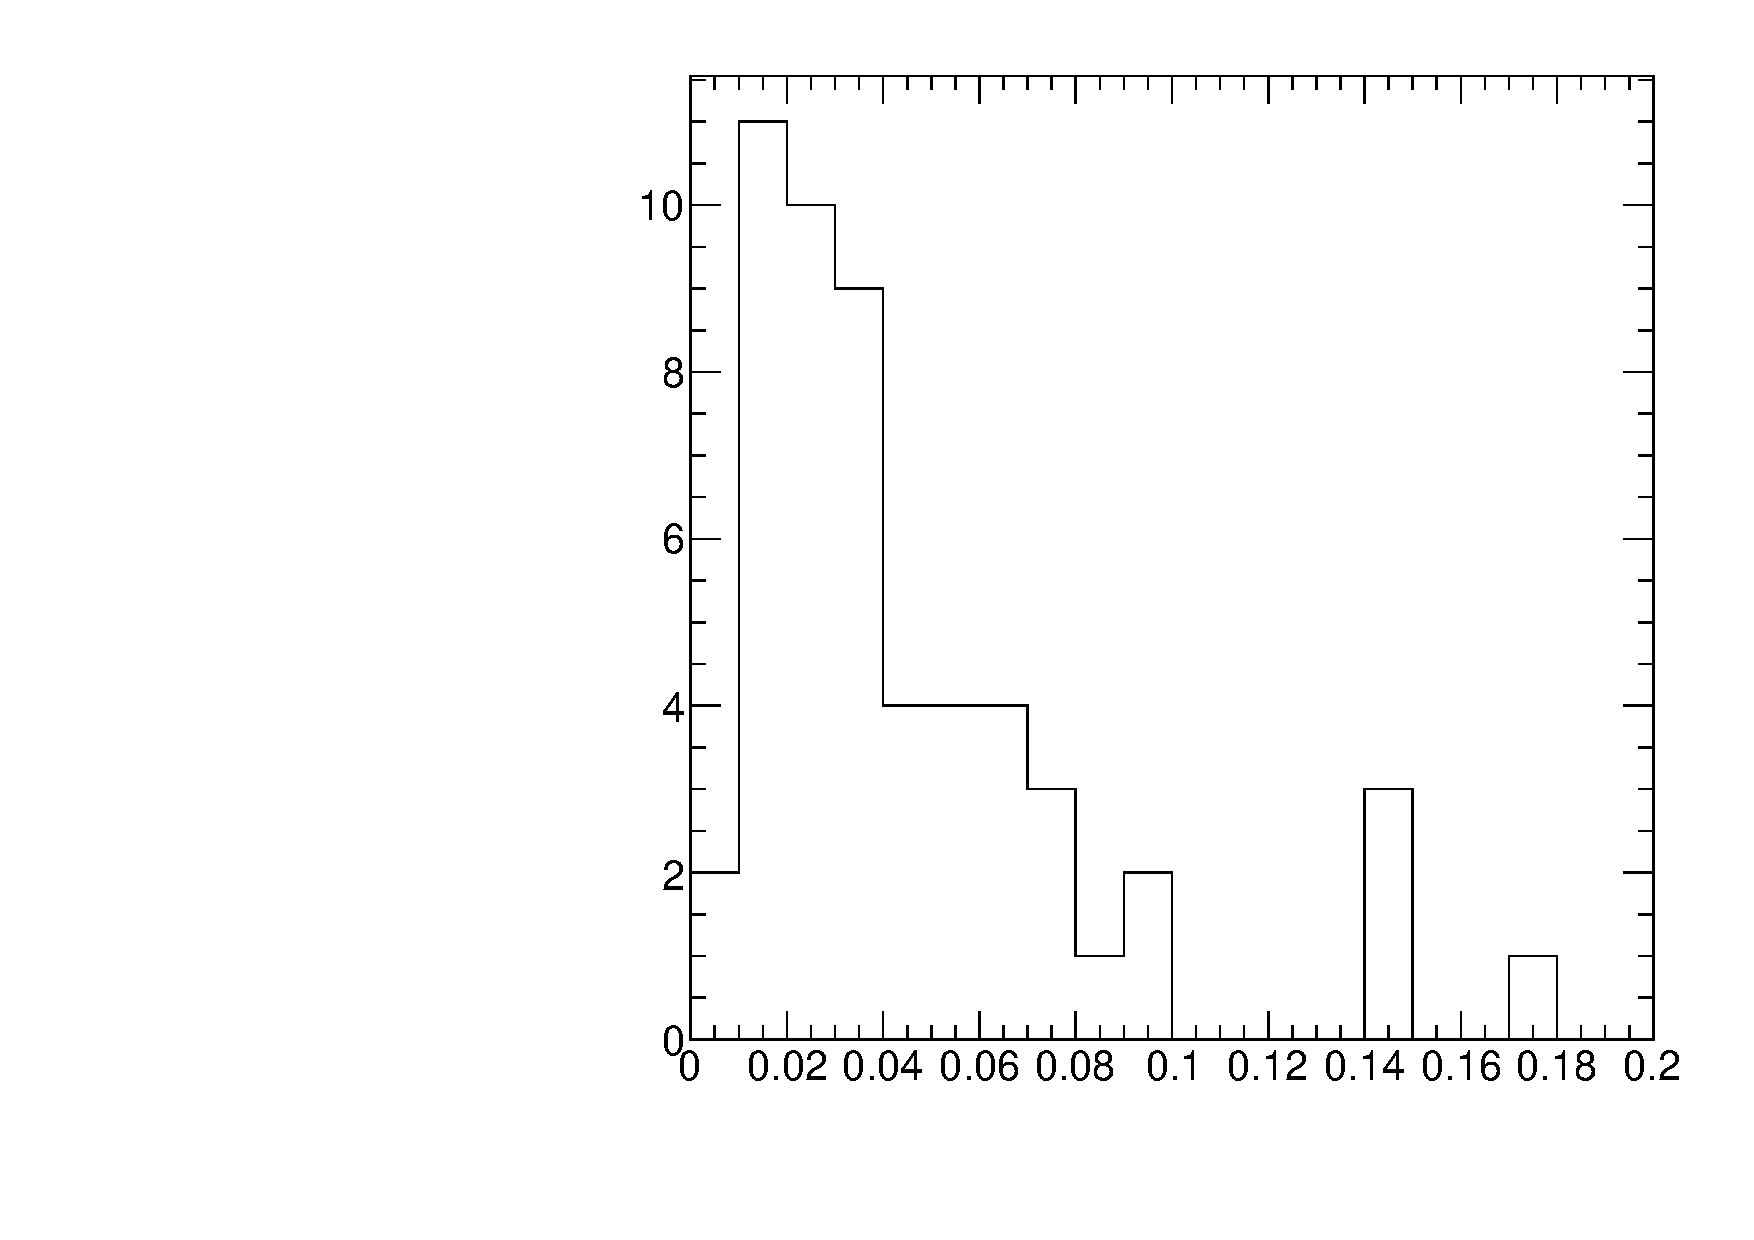
\includegraphics[width=0.3\textwidth]{Figures/AfterBDTCut_docatrk_Barrel.pdf}
  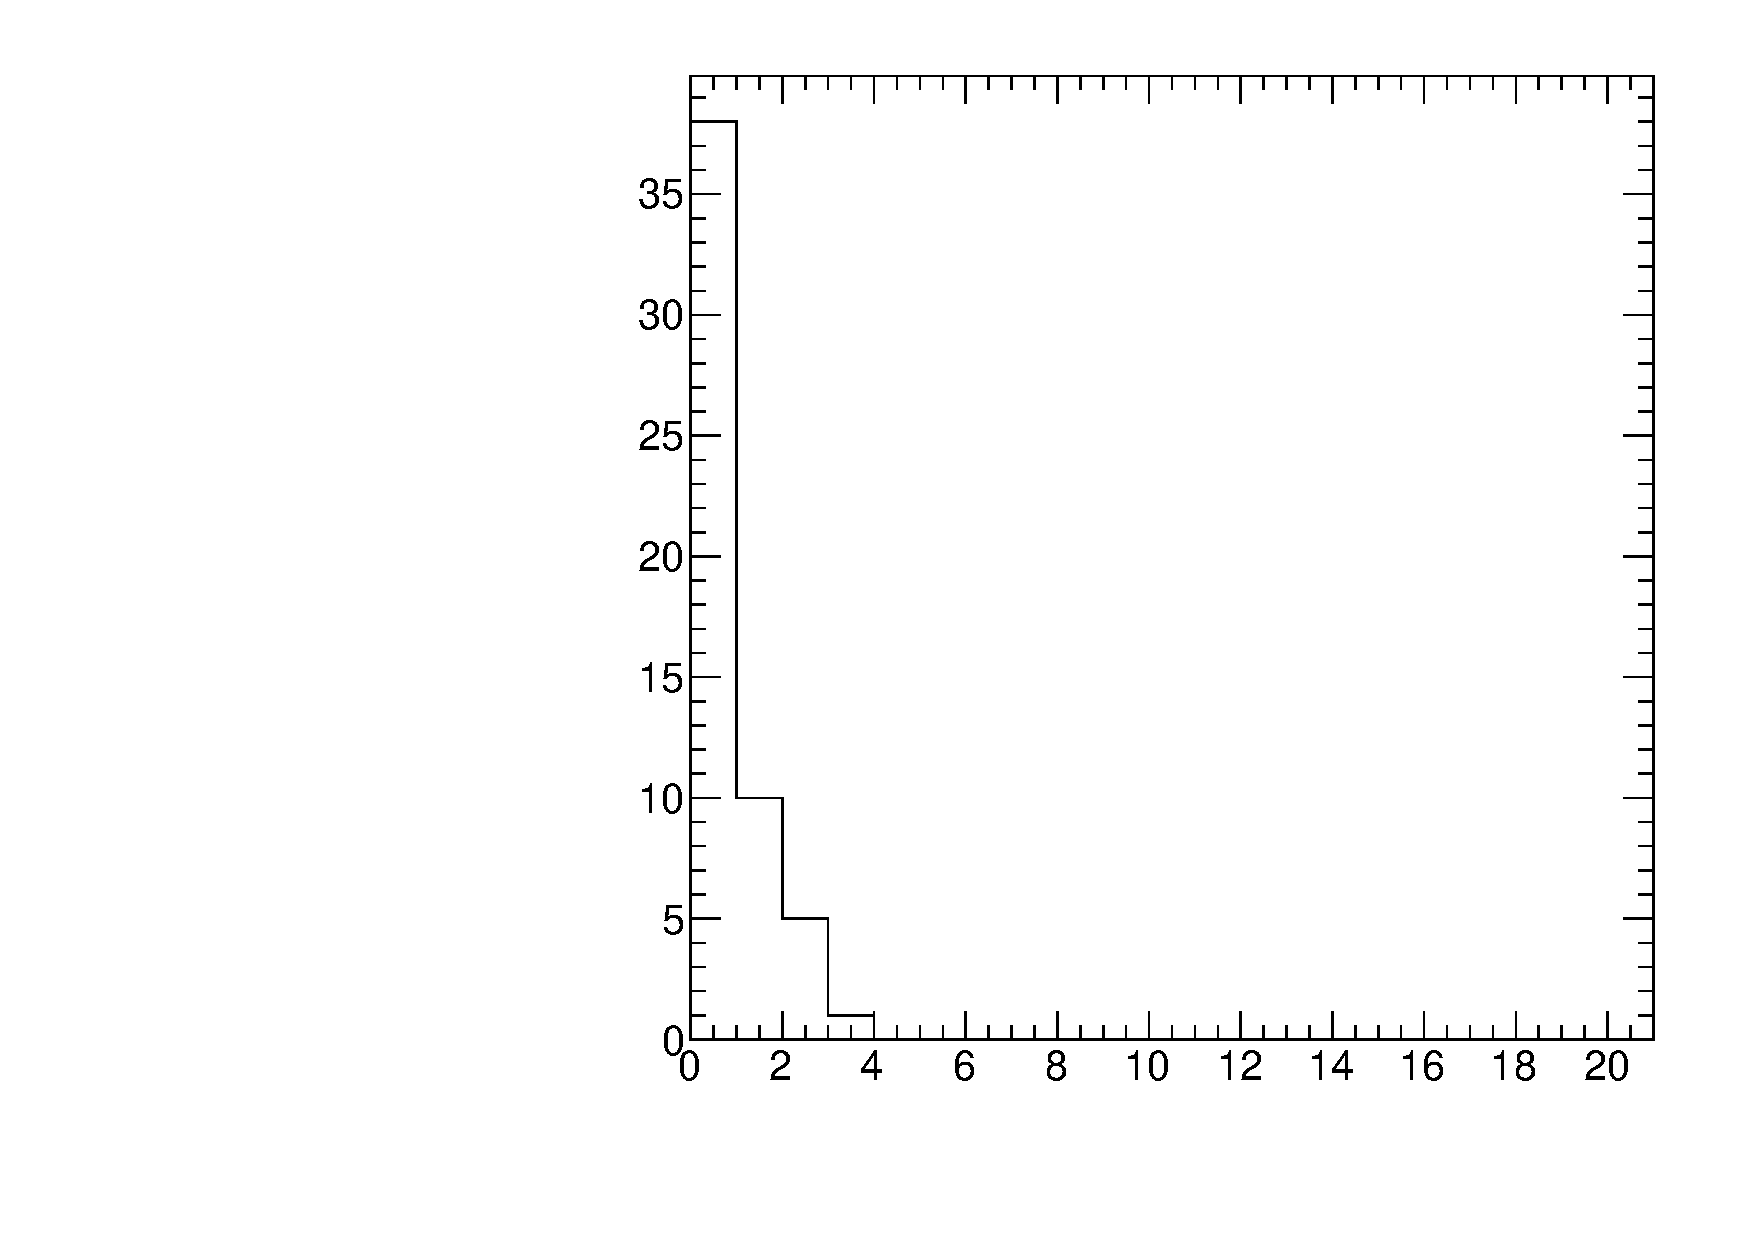
\includegraphics[width=0.3\textwidth]{Figures/AfterBDTCut_closetrk_Barrel.pdf}
  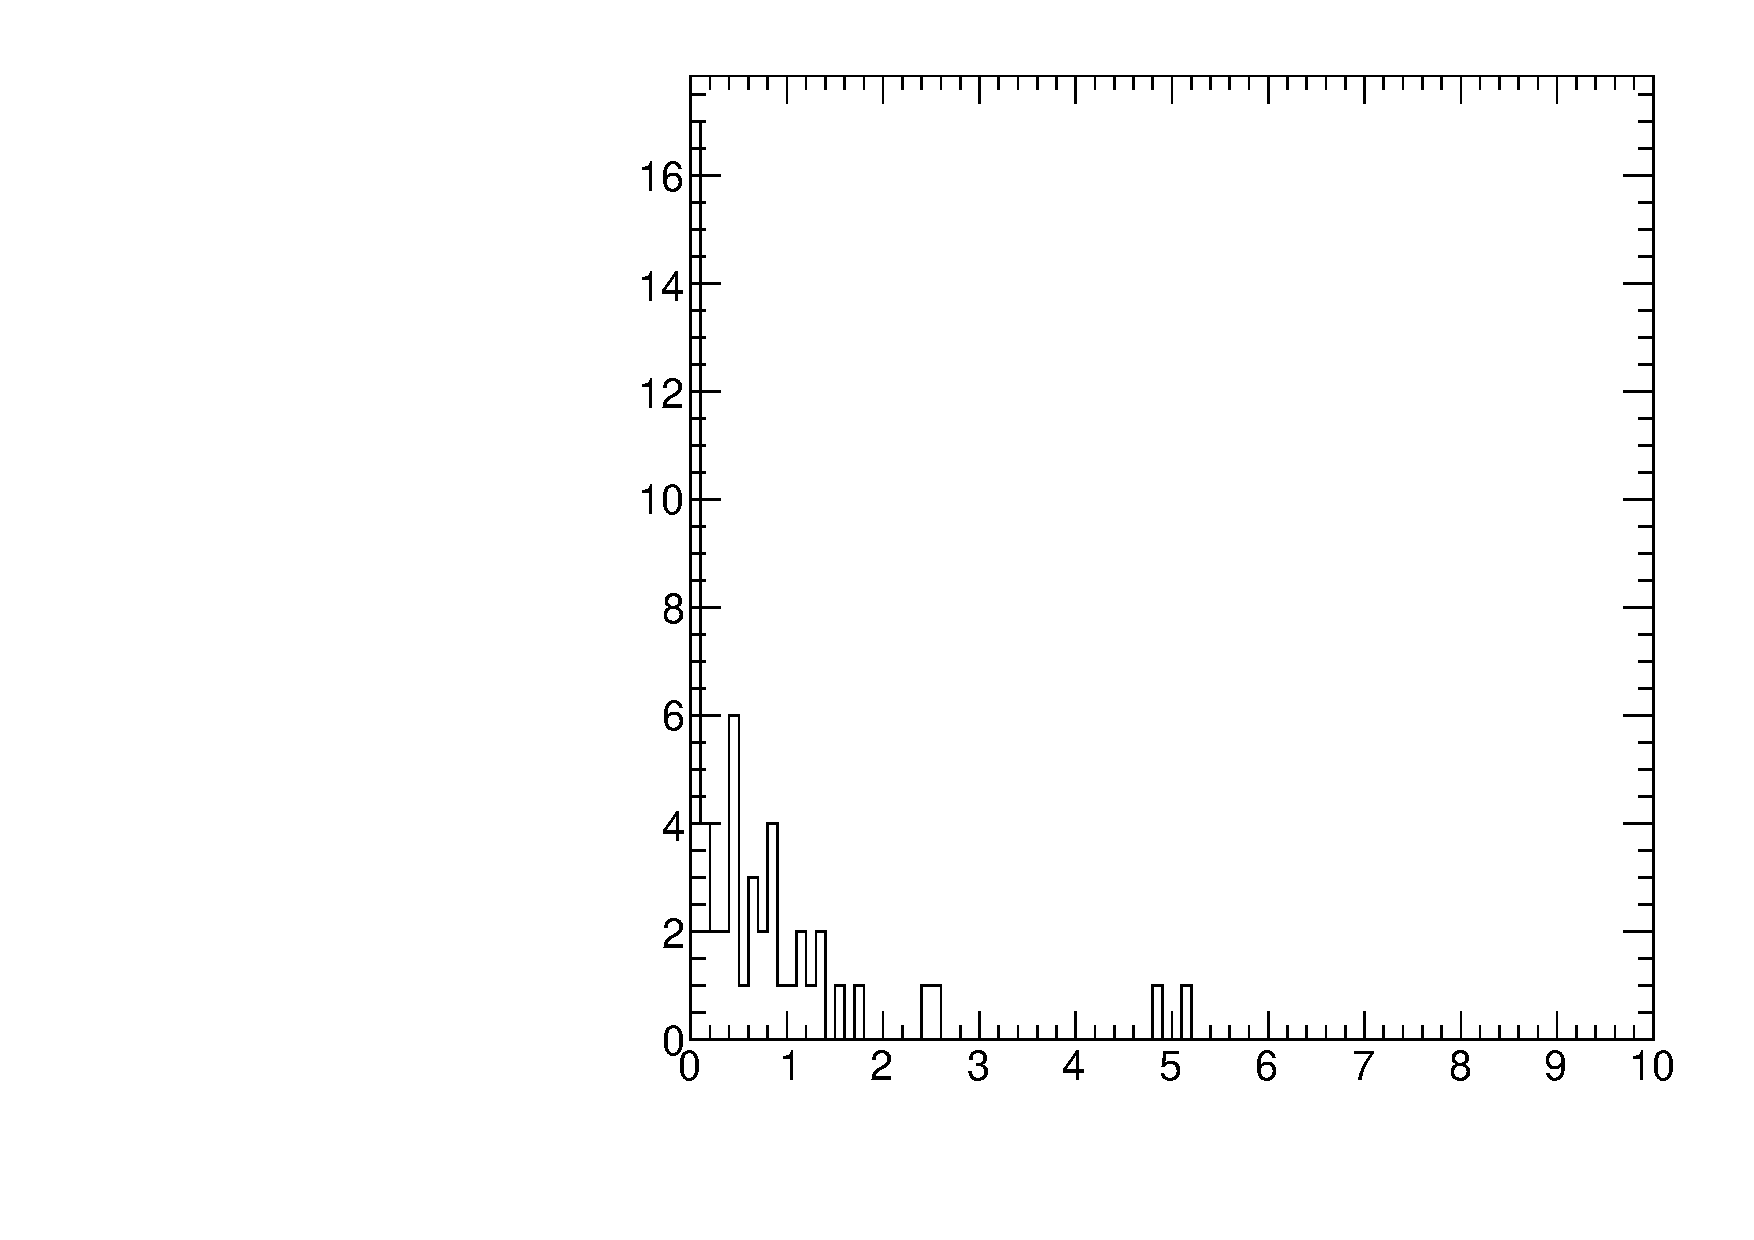
\includegraphics[width=0.3\textwidth]{Figures/AfterBDTCut_chi2dof_Barrel.pdf}
  \caption{Variable distributions for the barrel after BDT cuts on blinded data.}
  \label{fig:AfterBDTCutVariablesBarrelBlinded}
\end{figure}

\begin{figure}
  \centering
  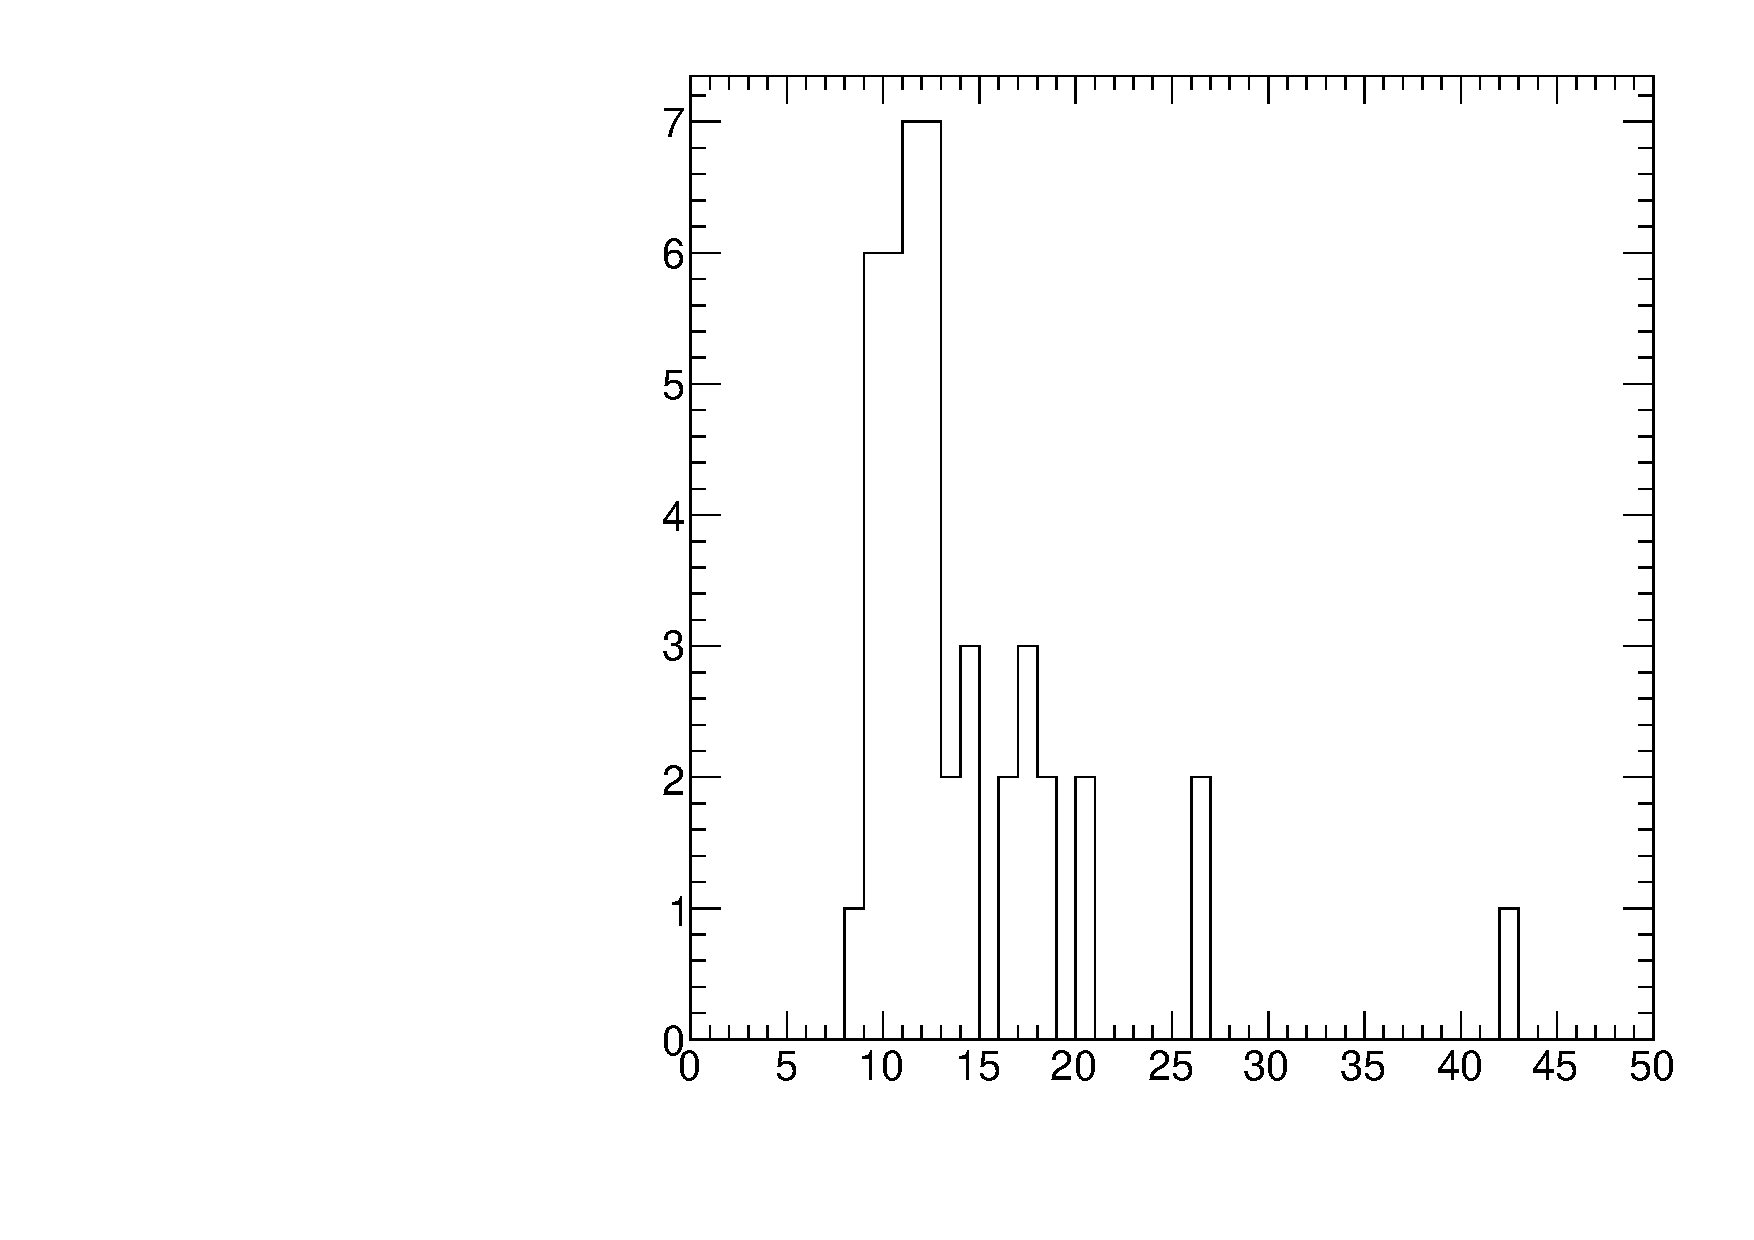
\includegraphics[width=0.3\textwidth]{Figures/AfterBDTCut_pt_Endcaps.pdf}
  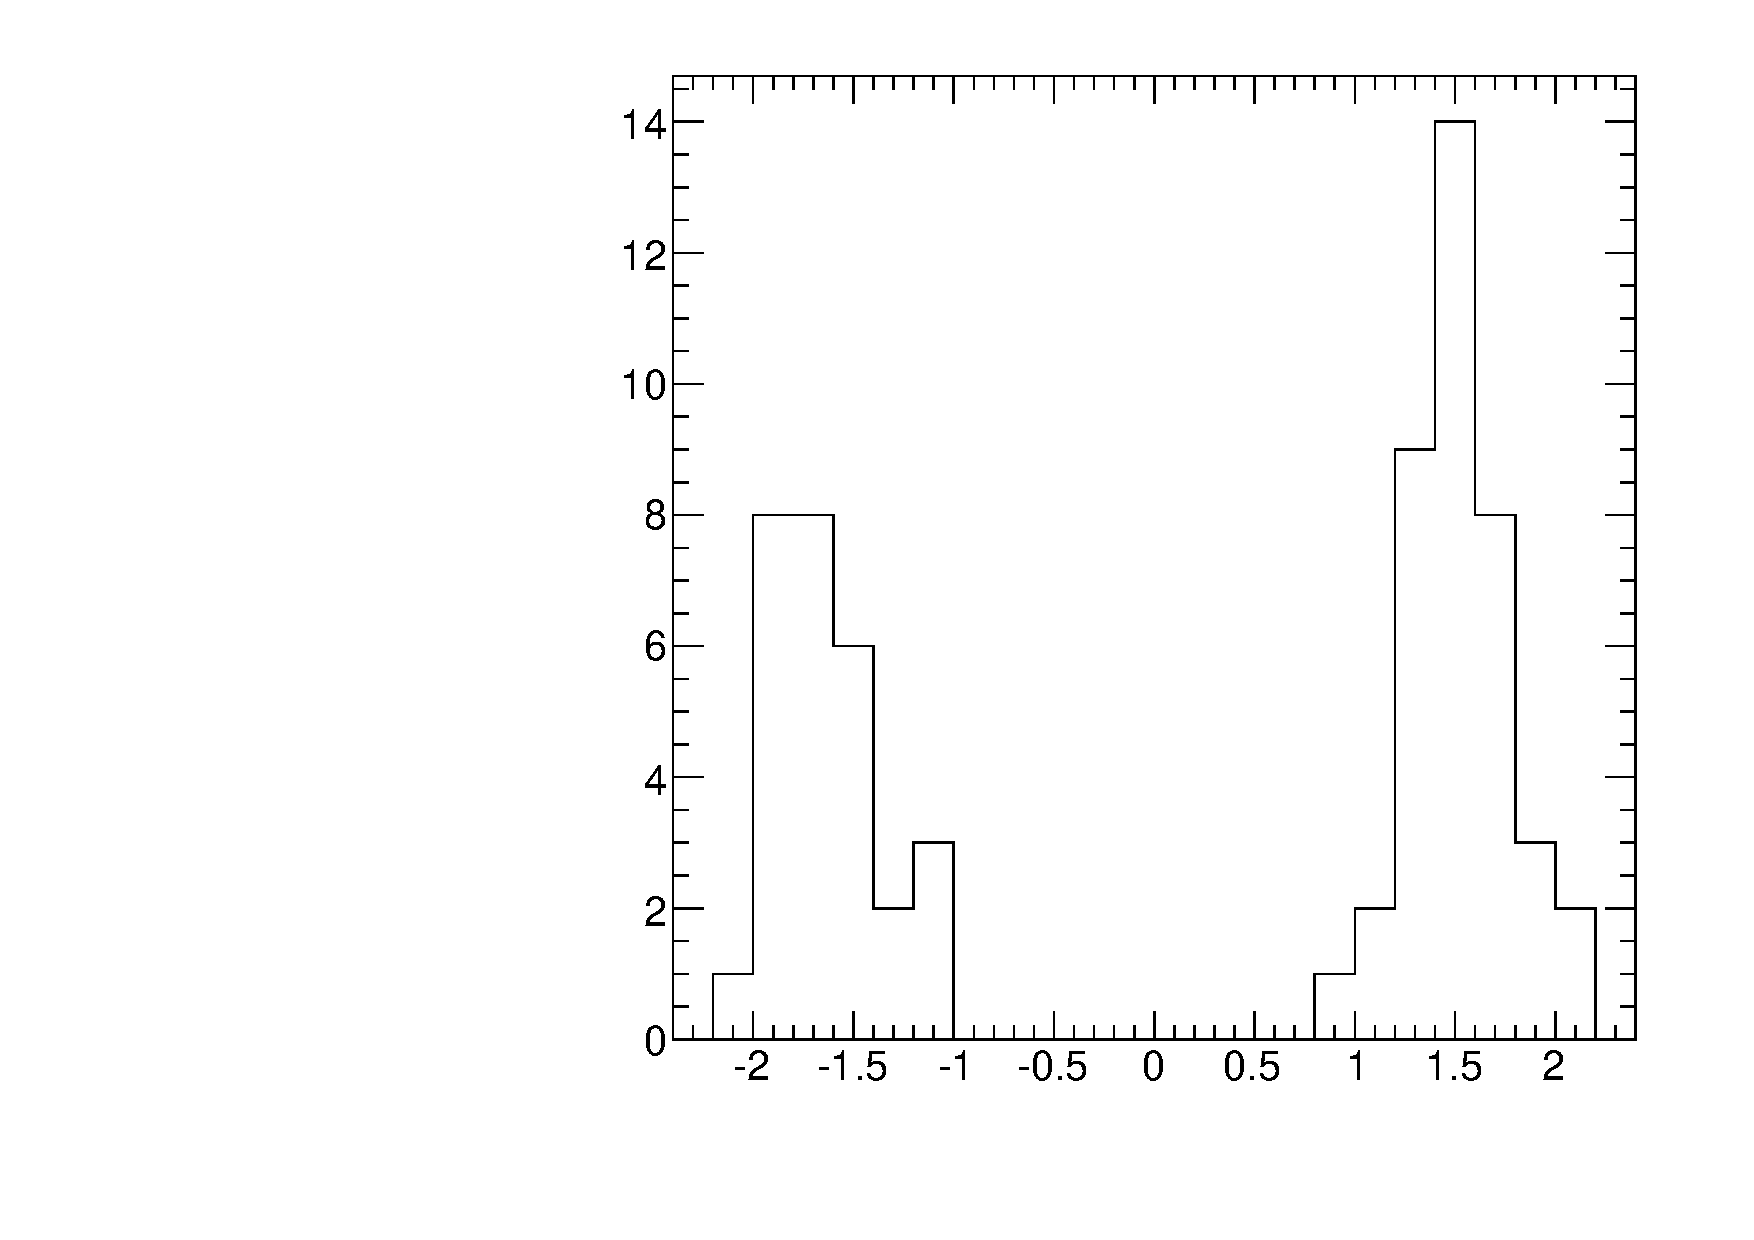
\includegraphics[width=0.3\textwidth]{Figures/AfterBDTCut_eta_Endcaps.pdf}
  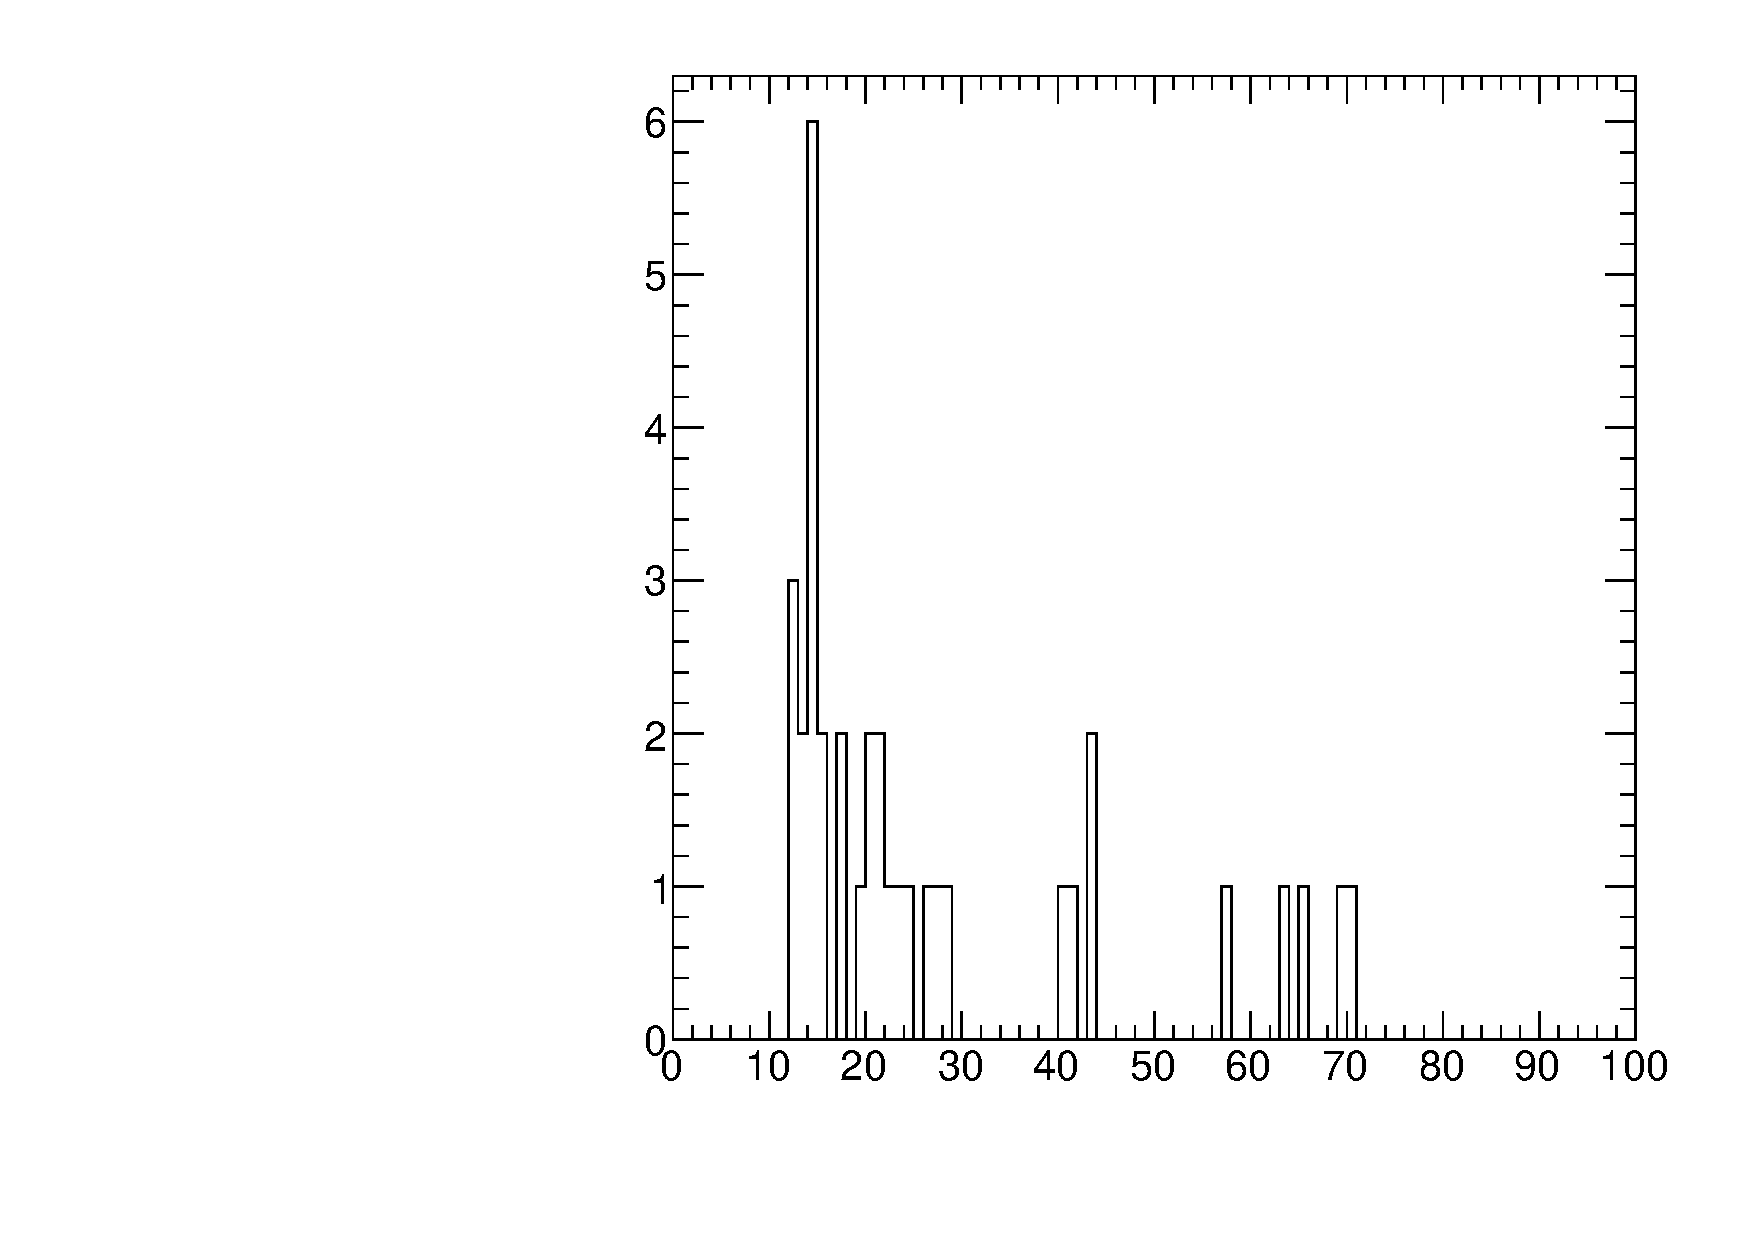
\includegraphics[width=0.3\textwidth]{Figures/AfterBDTCut_fls3d_Endcaps.pdf}
  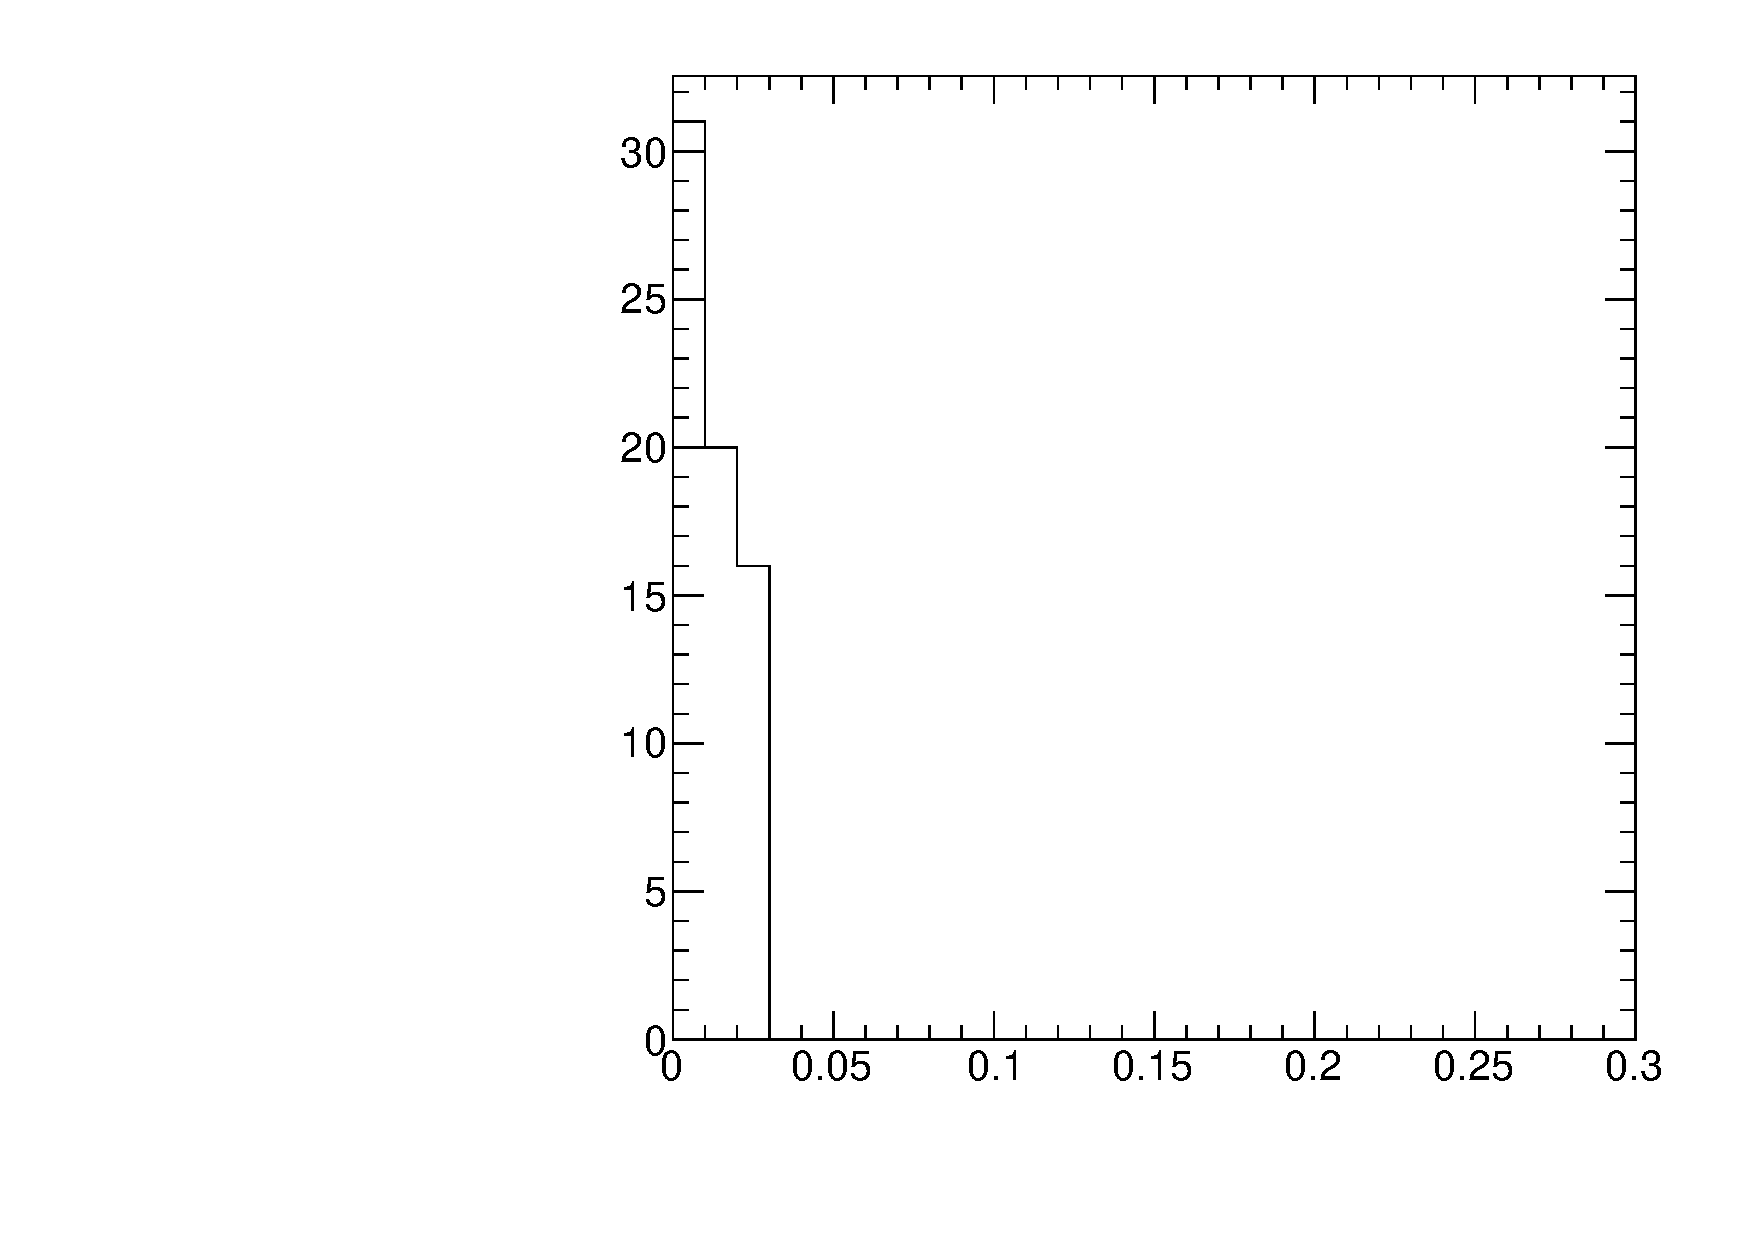
\includegraphics[width=0.3\textwidth]{Figures/AfterBDTCut_alpha_Endcaps.pdf}
  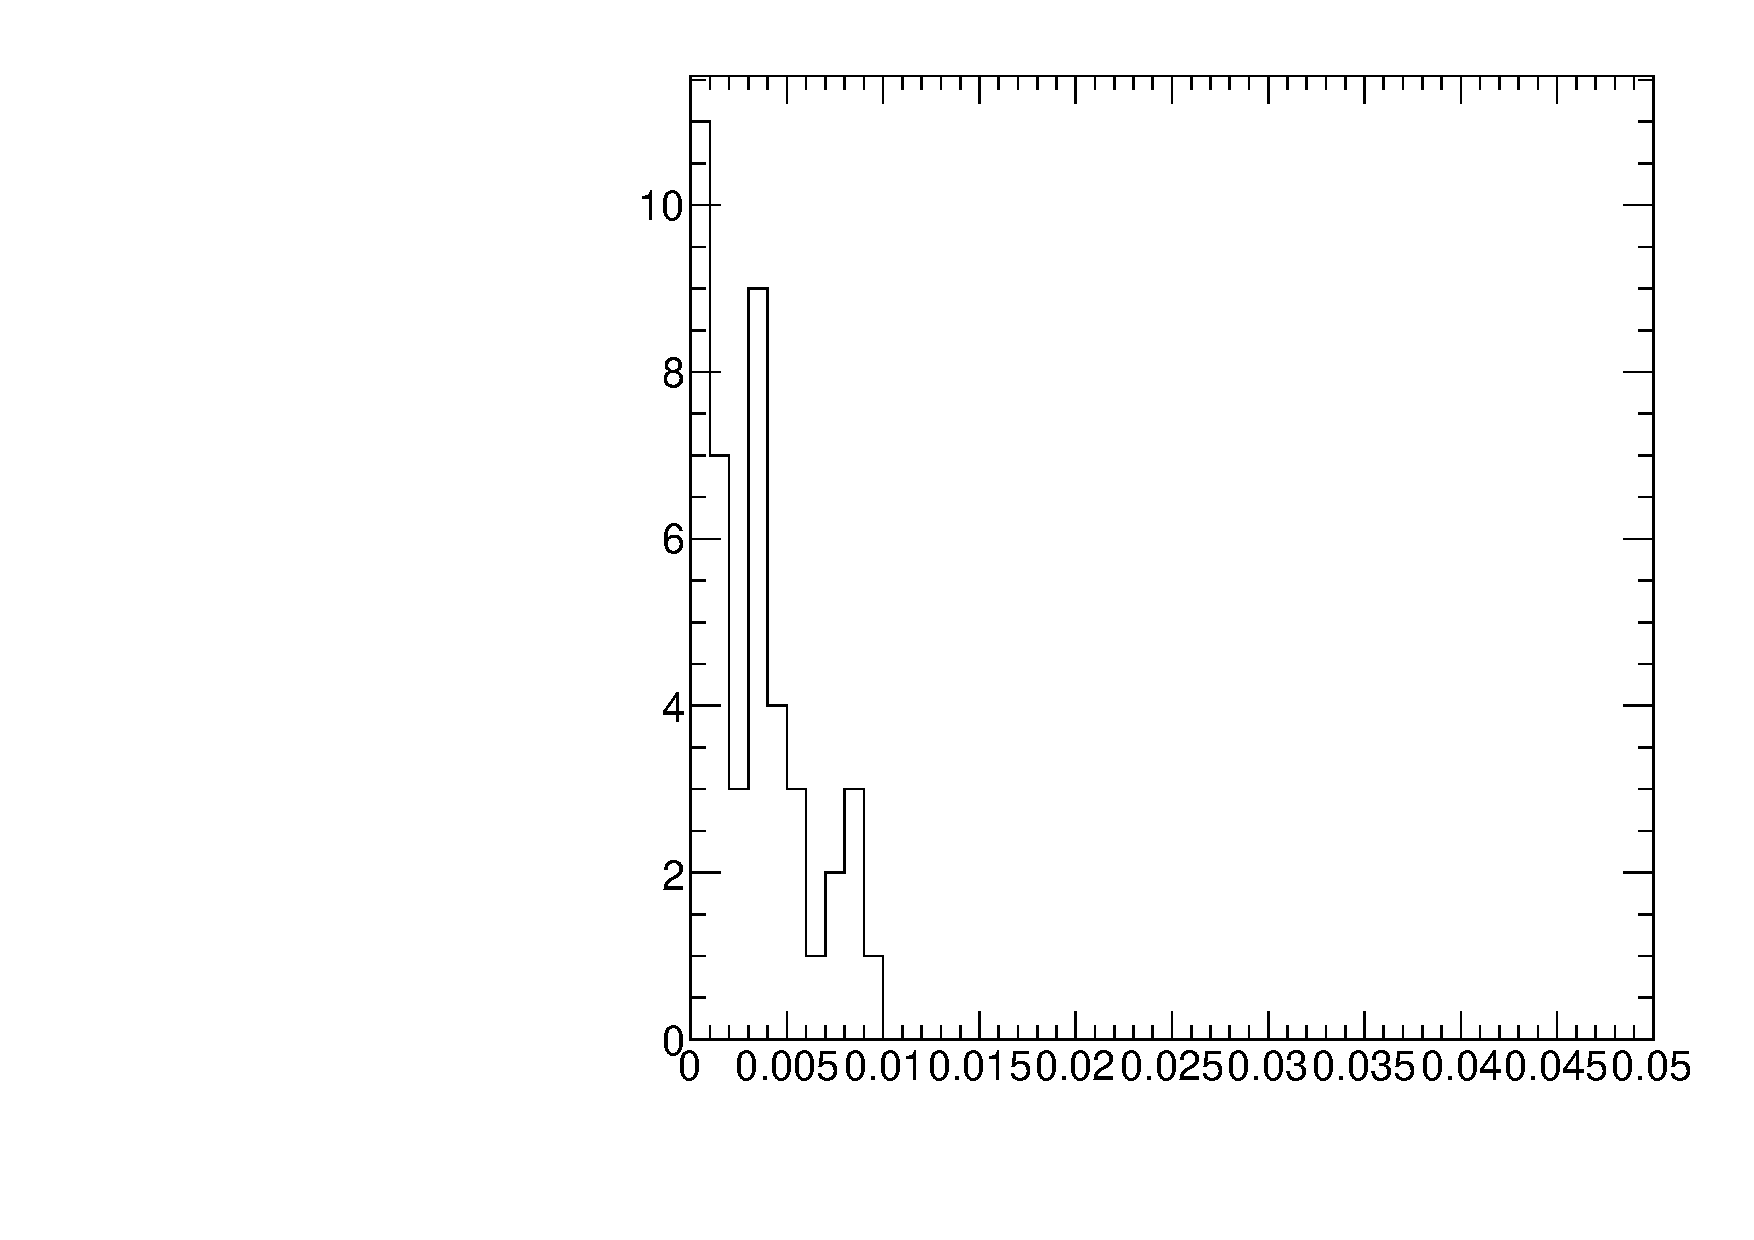
\includegraphics[width=0.3\textwidth]{Figures/AfterBDTCut_maxdoca_Endcaps.pdf}
  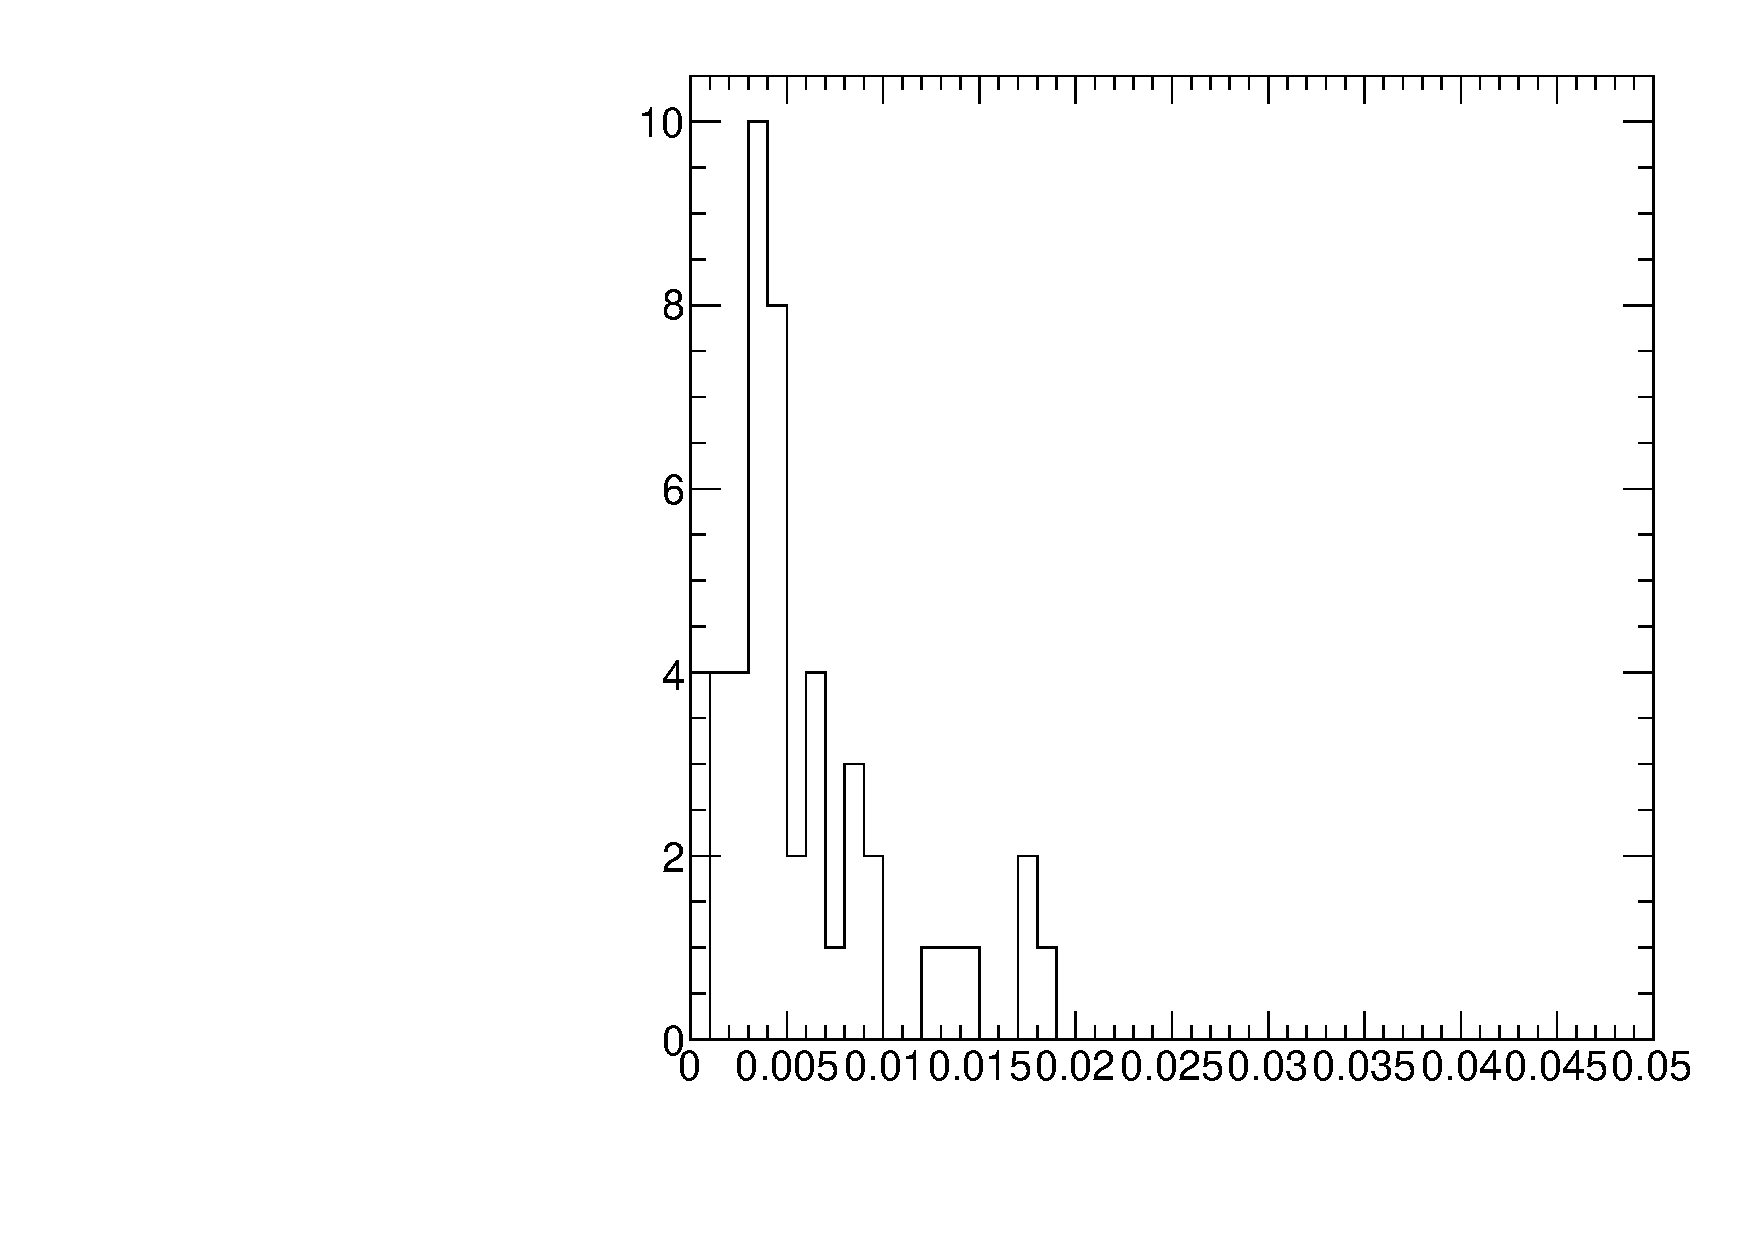
\includegraphics[width=0.3\textwidth]{Figures/AfterBDTCut_pvip_Endcaps.pdf}
  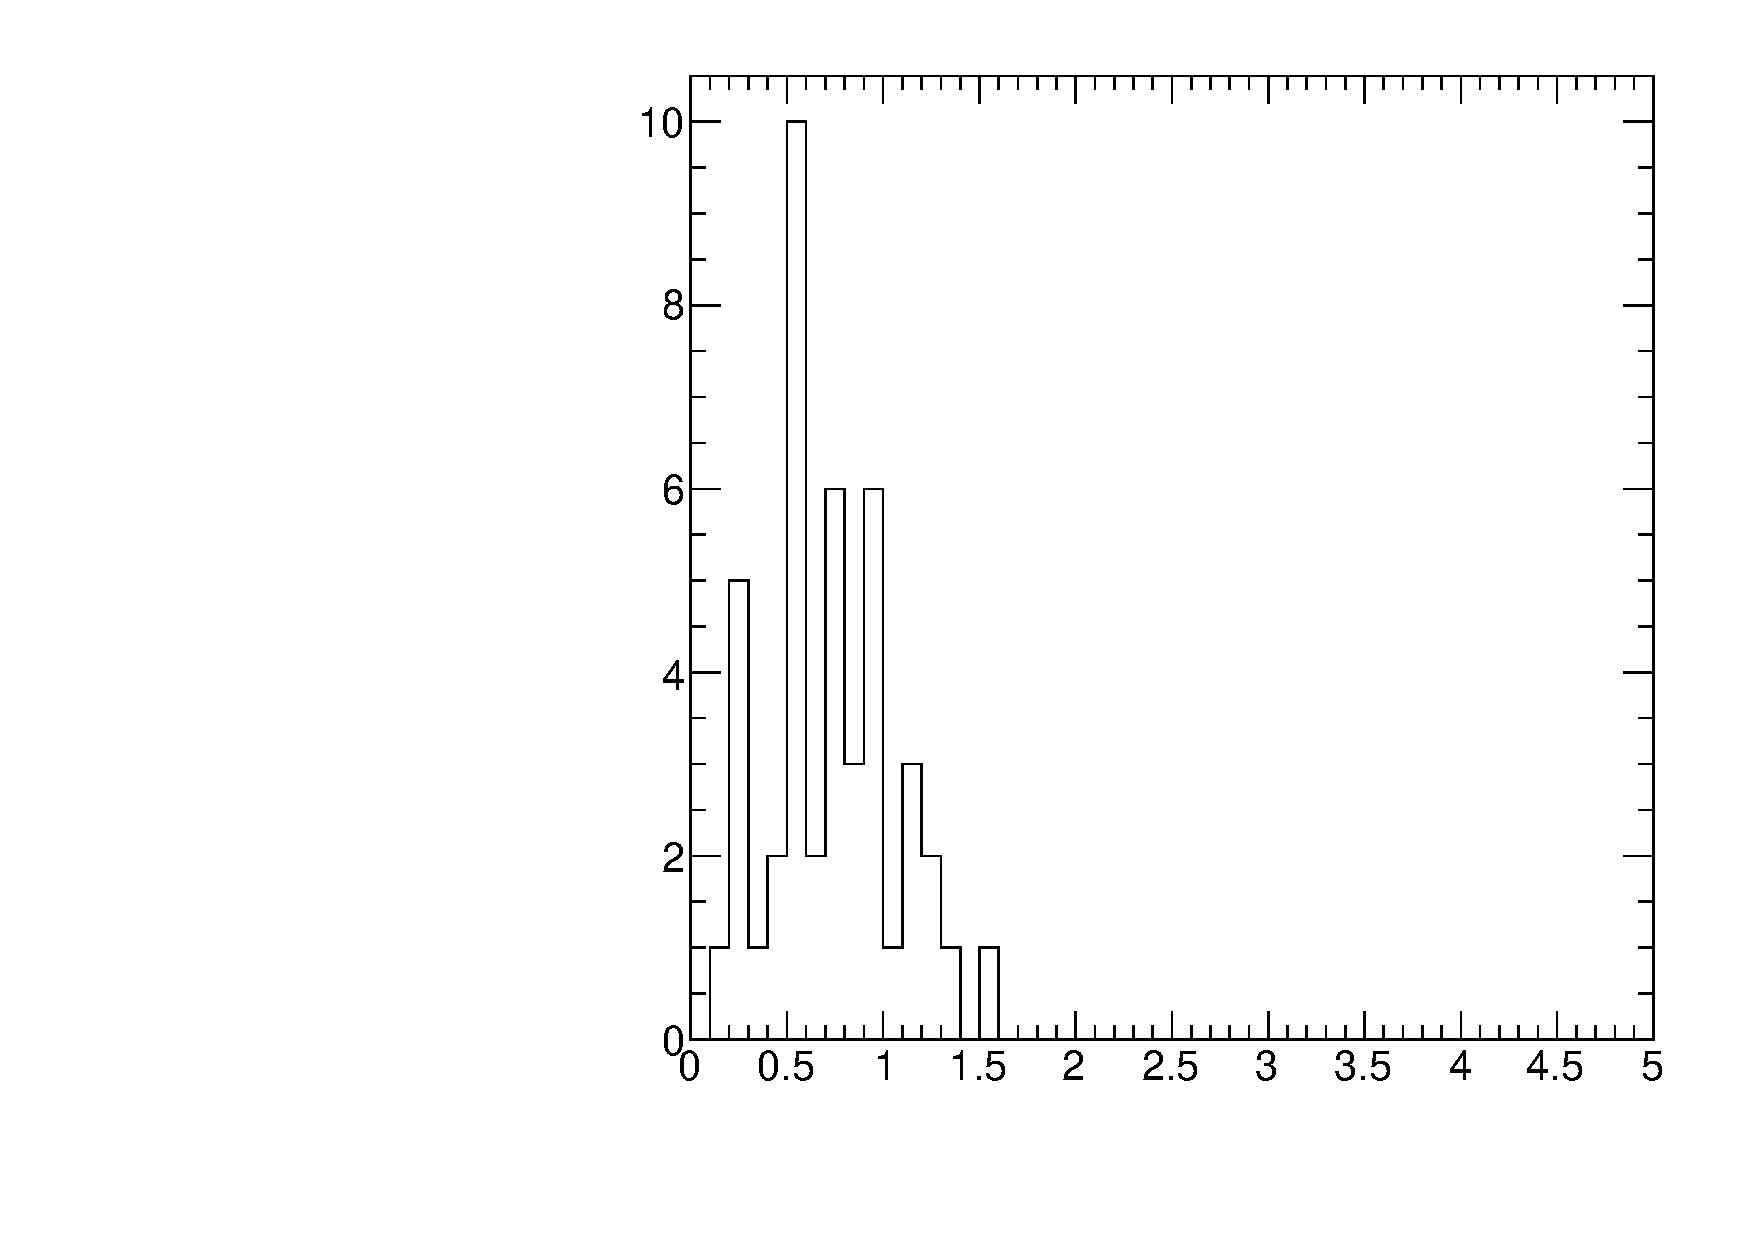
\includegraphics[width=0.3\textwidth]{Figures/AfterBDTCut_pvips_Endcaps.pdf}
  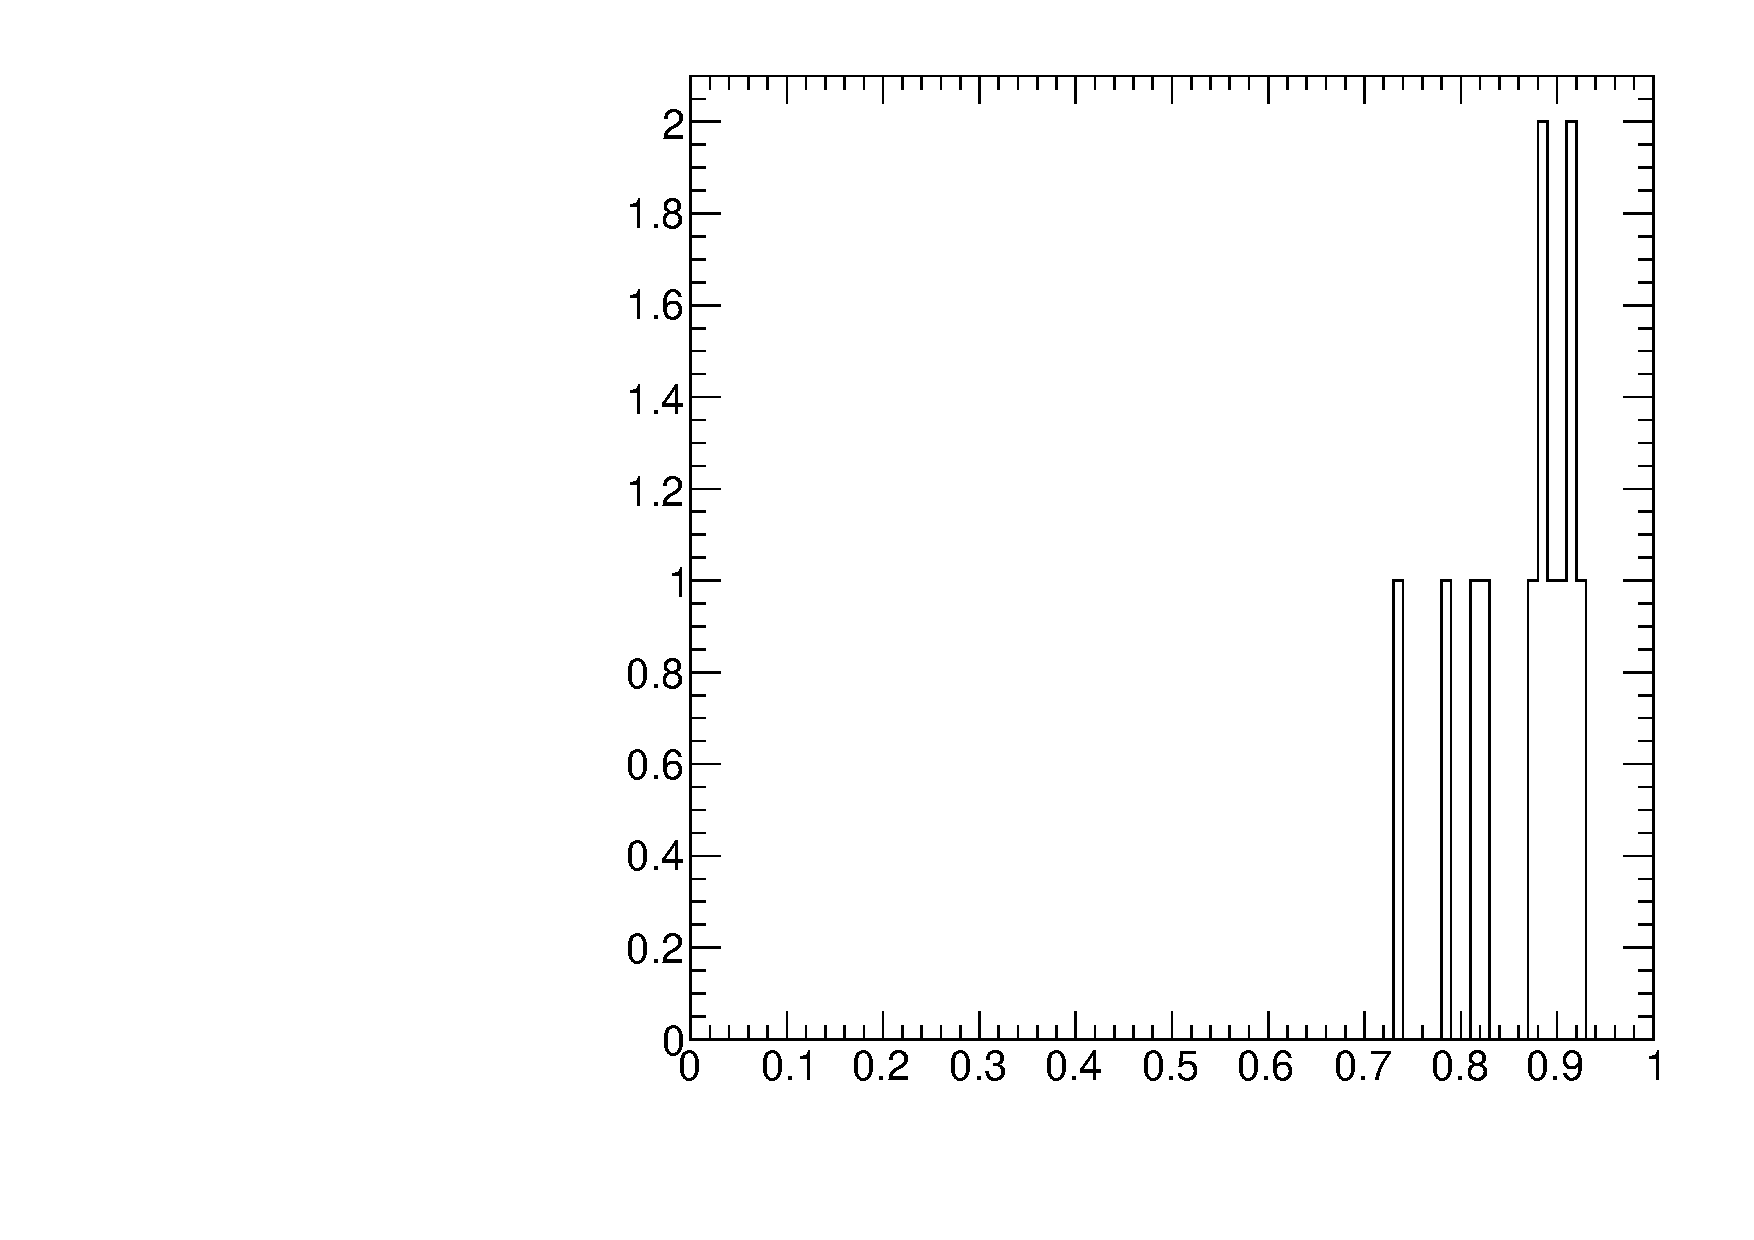
\includegraphics[width=0.3\textwidth]{Figures/AfterBDTCut_iso_Endcaps.pdf}
  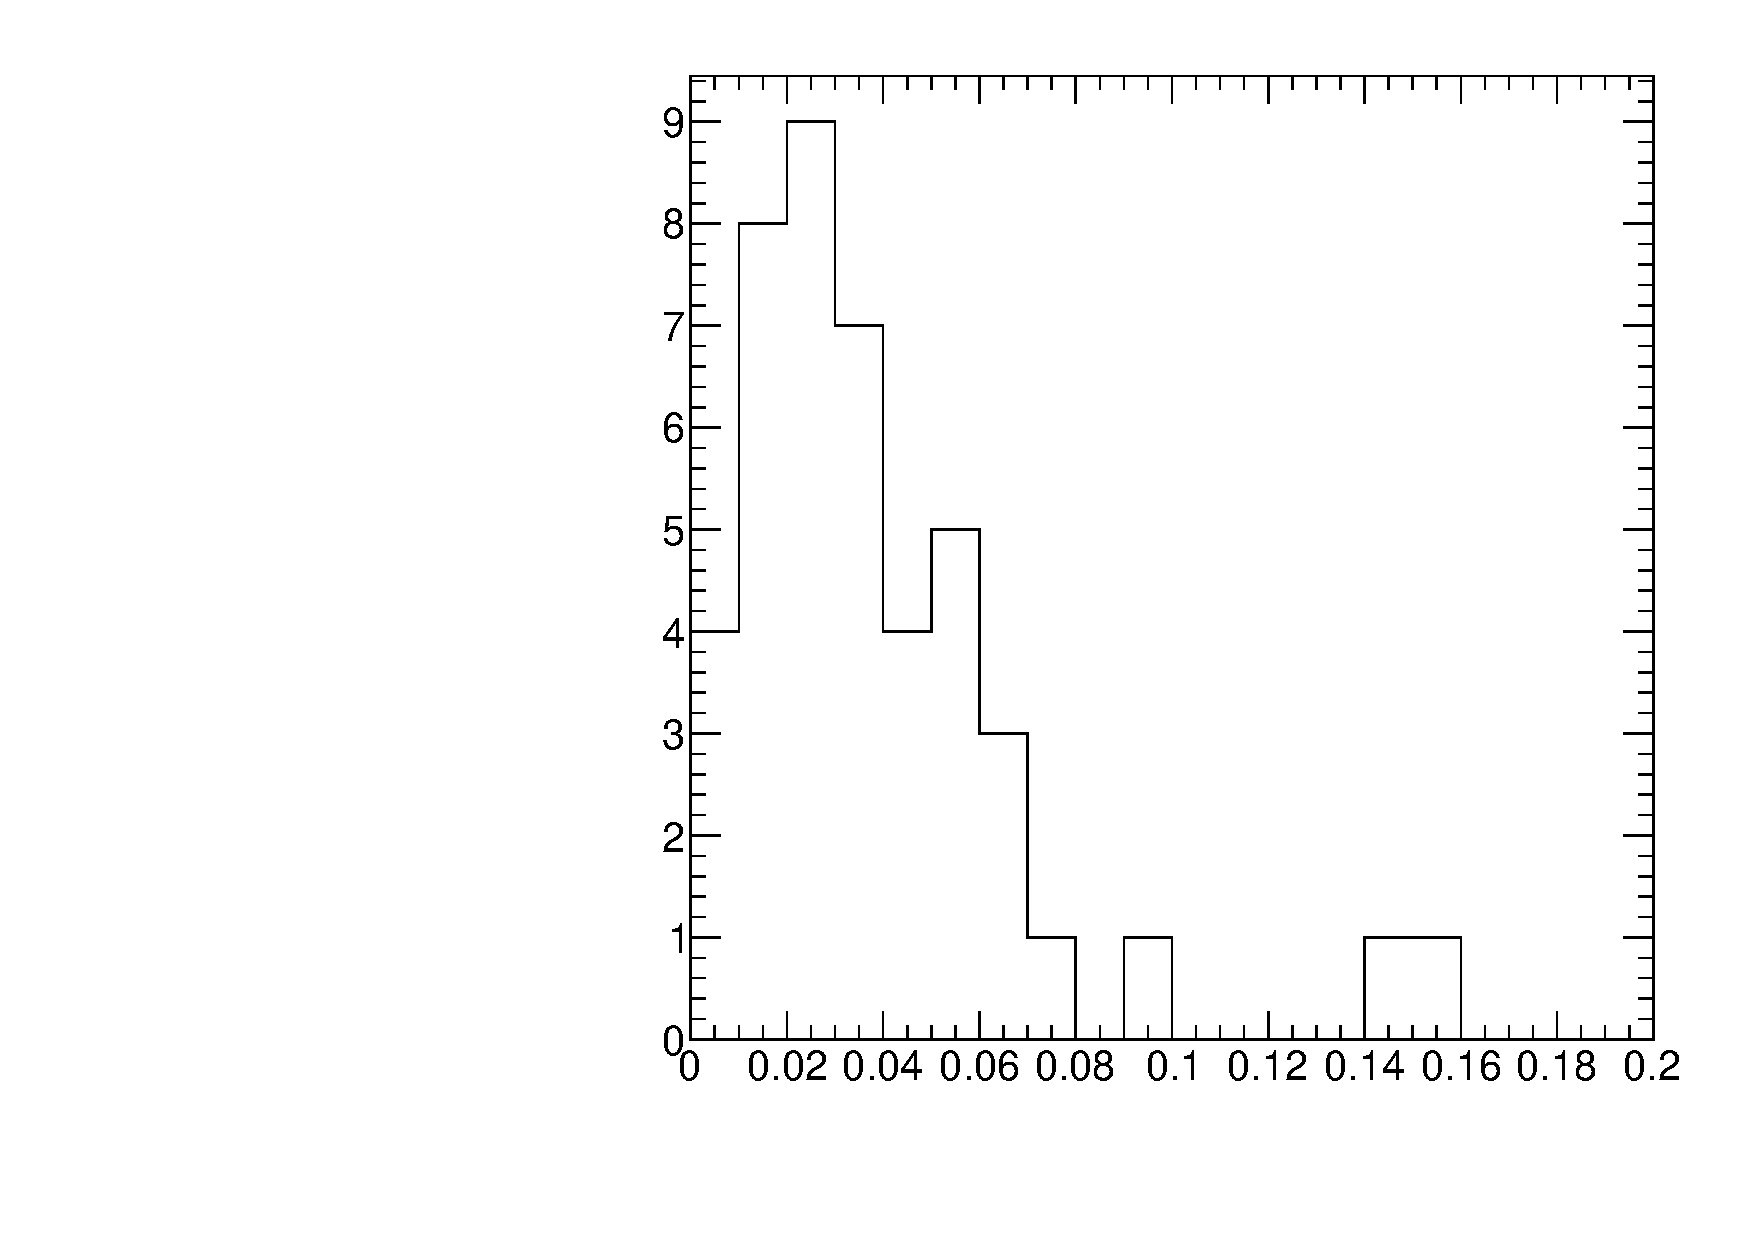
\includegraphics[width=0.3\textwidth]{Figures/AfterBDTCut_docatrk_Endcaps.pdf}
  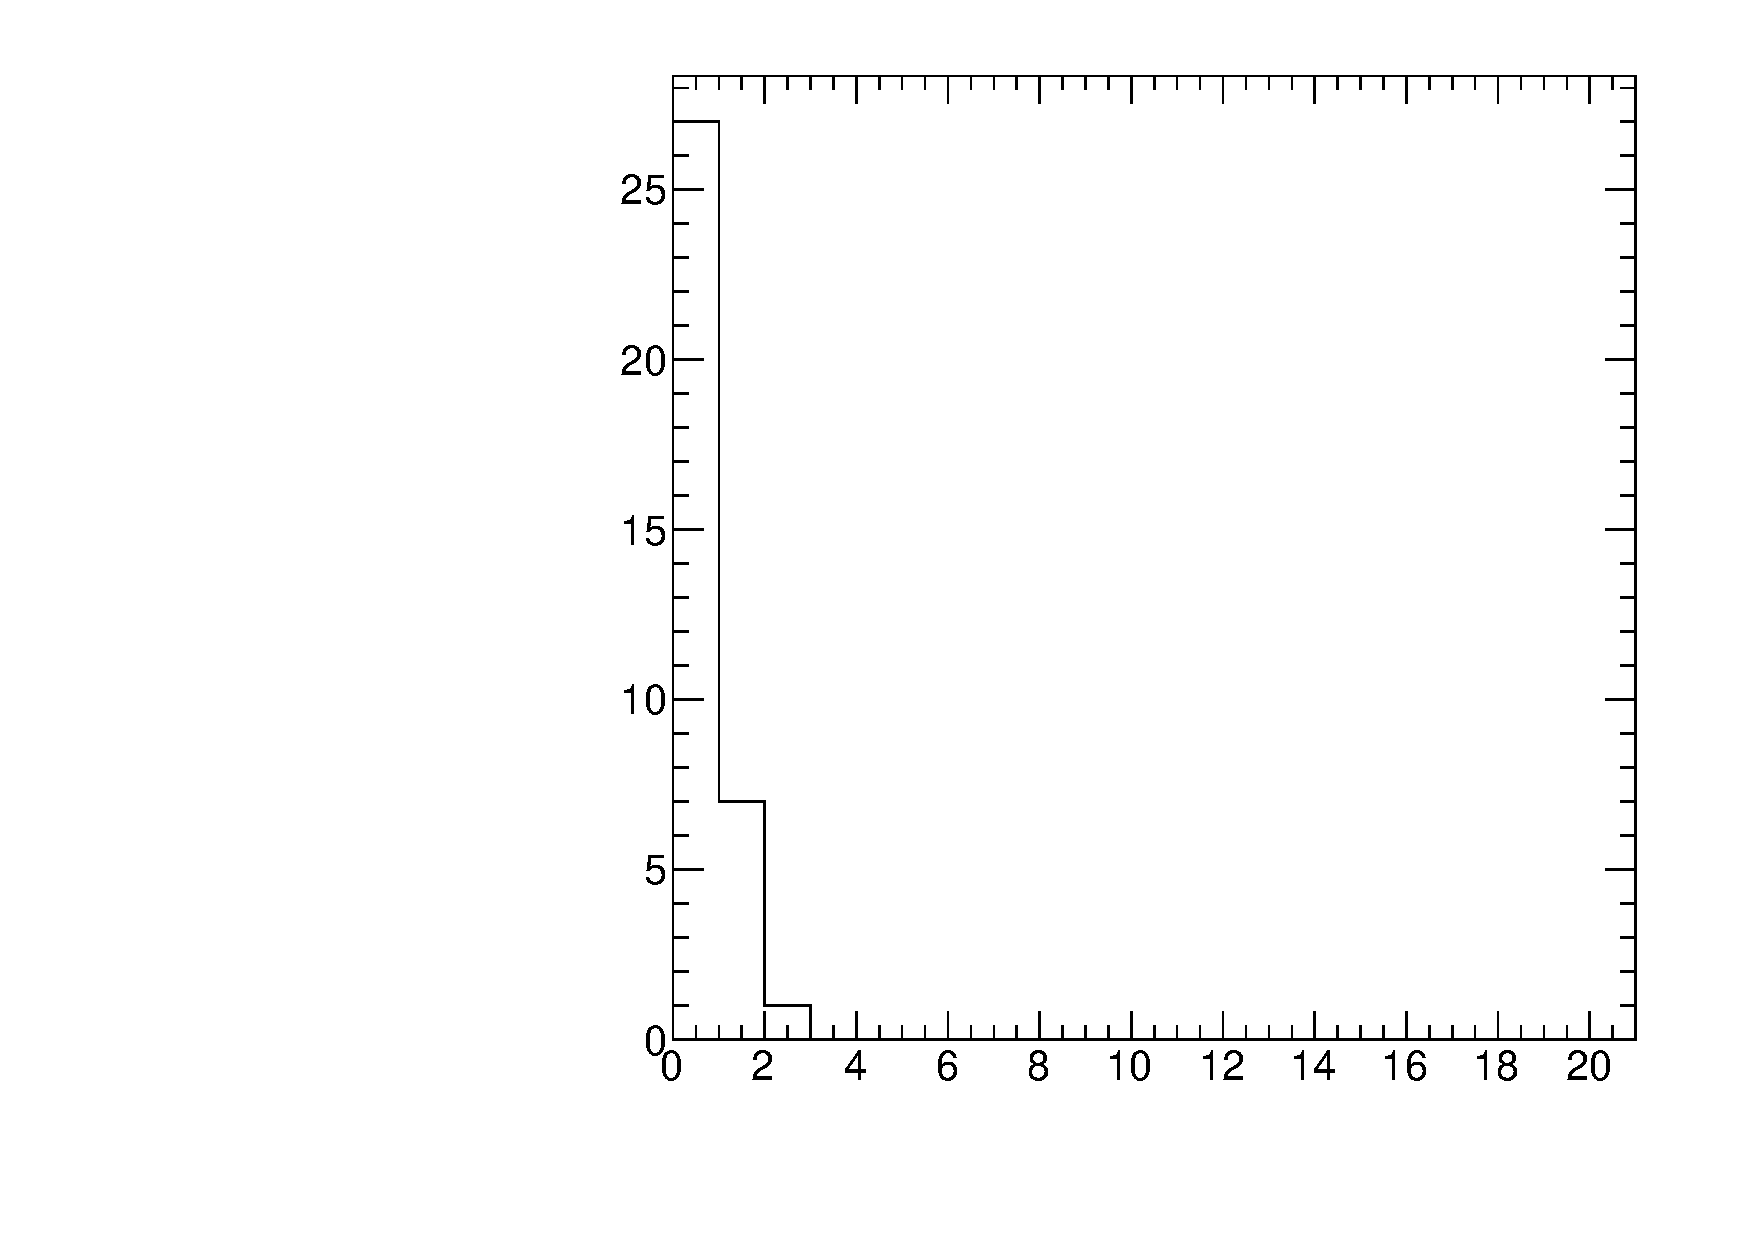
\includegraphics[width=0.3\textwidth]{Figures/AfterBDTCut_closetrk_Endcaps.pdf}
  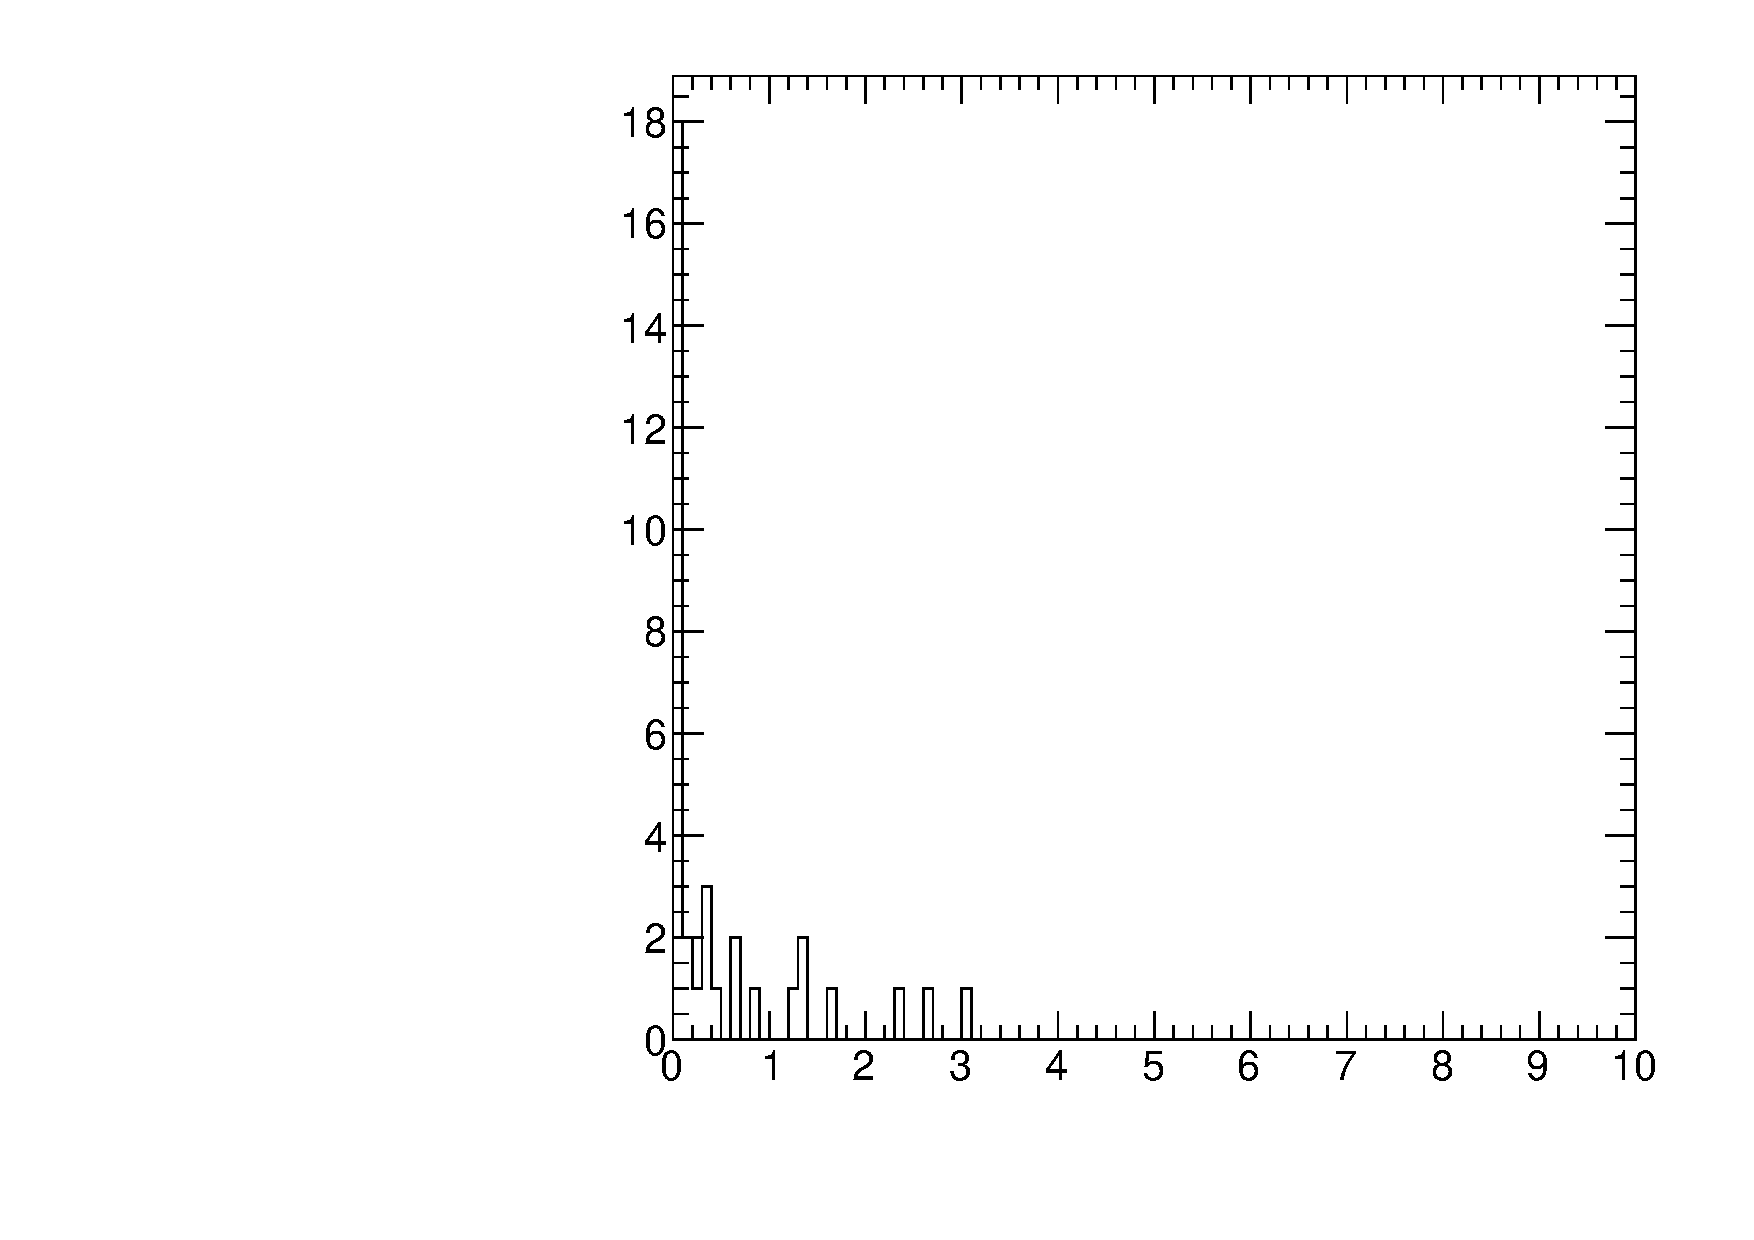
\includegraphics[width=0.3\textwidth]{Figures/AfterBDTCut_chi2dof_Endcaps.pdf}
  \caption{Variable distributions for the endcaps after BDT cuts on blinded data.}
  \label{fig:AfterBDTCutVariablesEndcapsBlinded}
\end{figure}

\begin{figure}
  \centering
  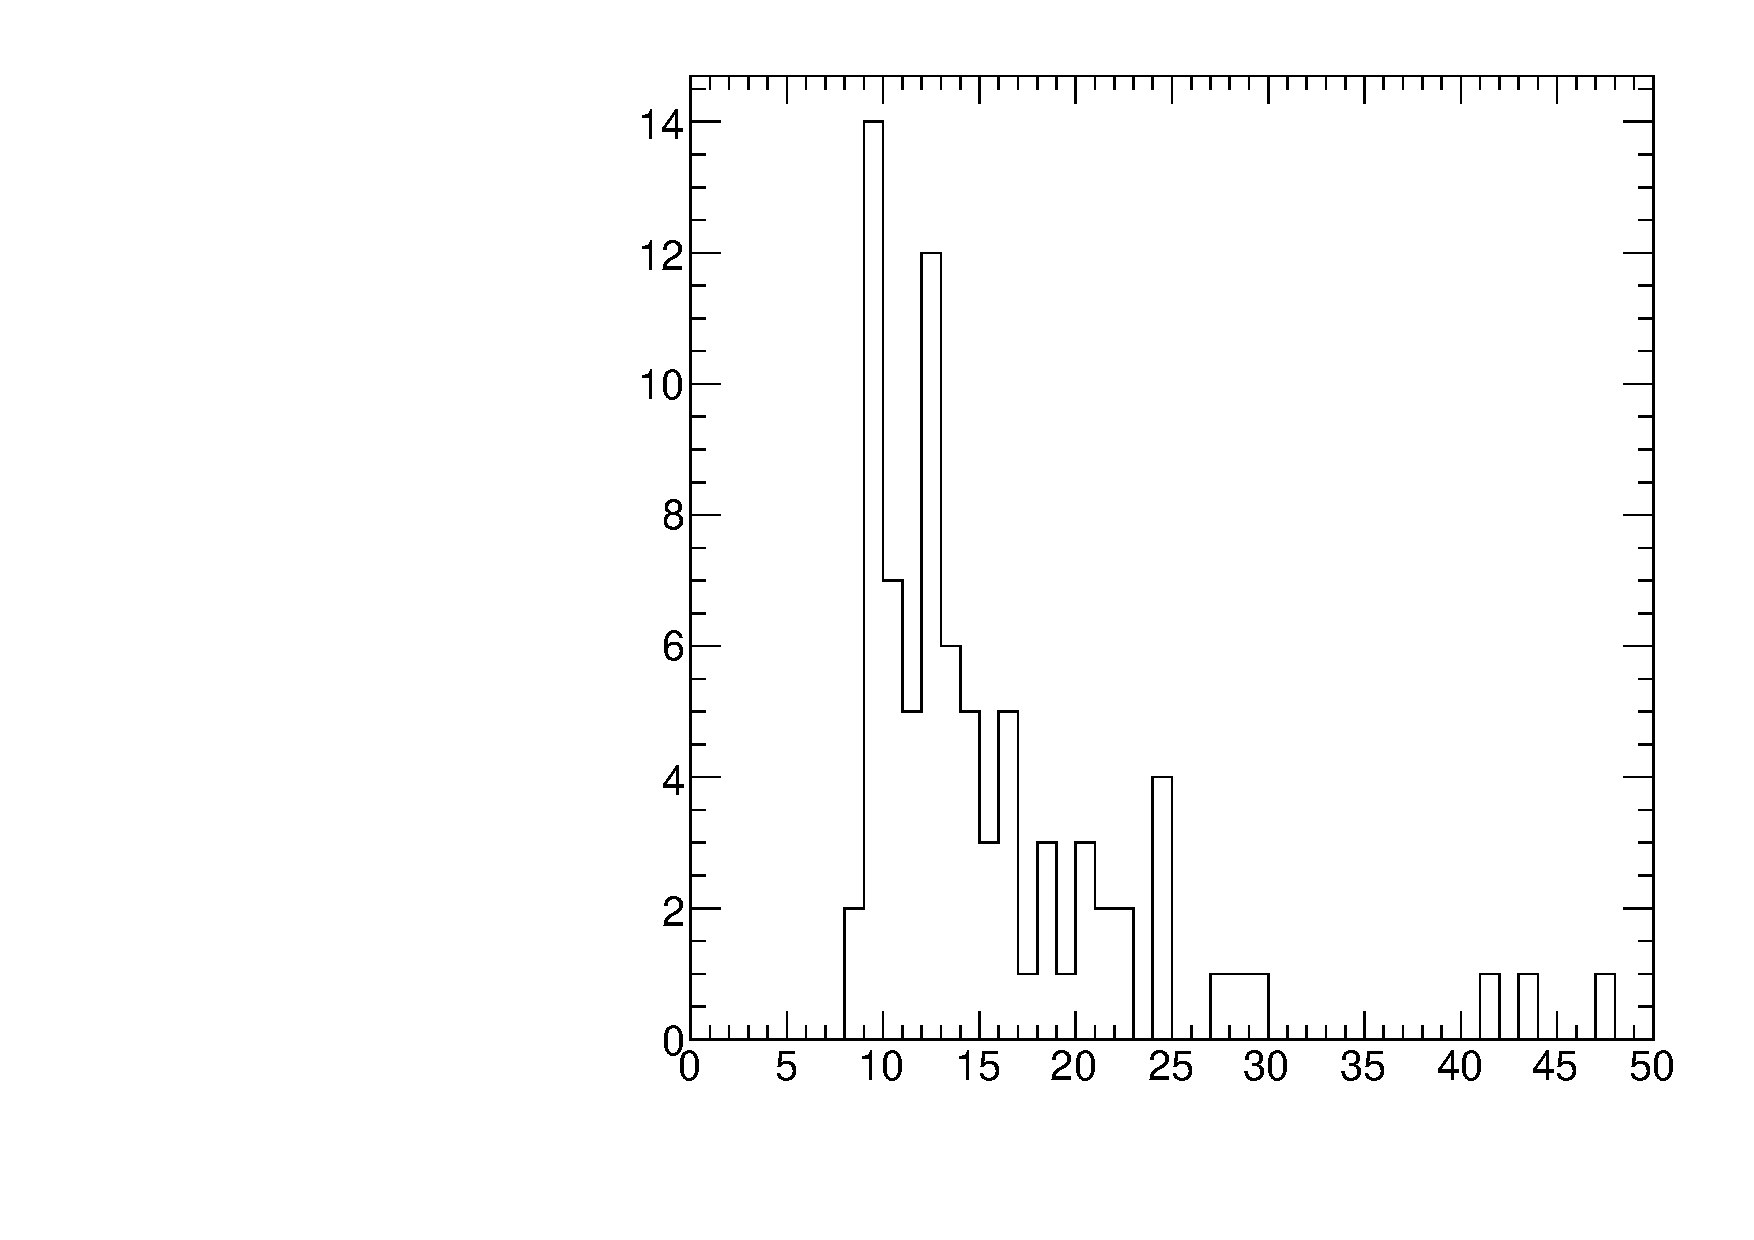
\includegraphics[width=0.3\textwidth]{Figures/AfterBDTCut_pt_BarrelUnblinded.pdf}
  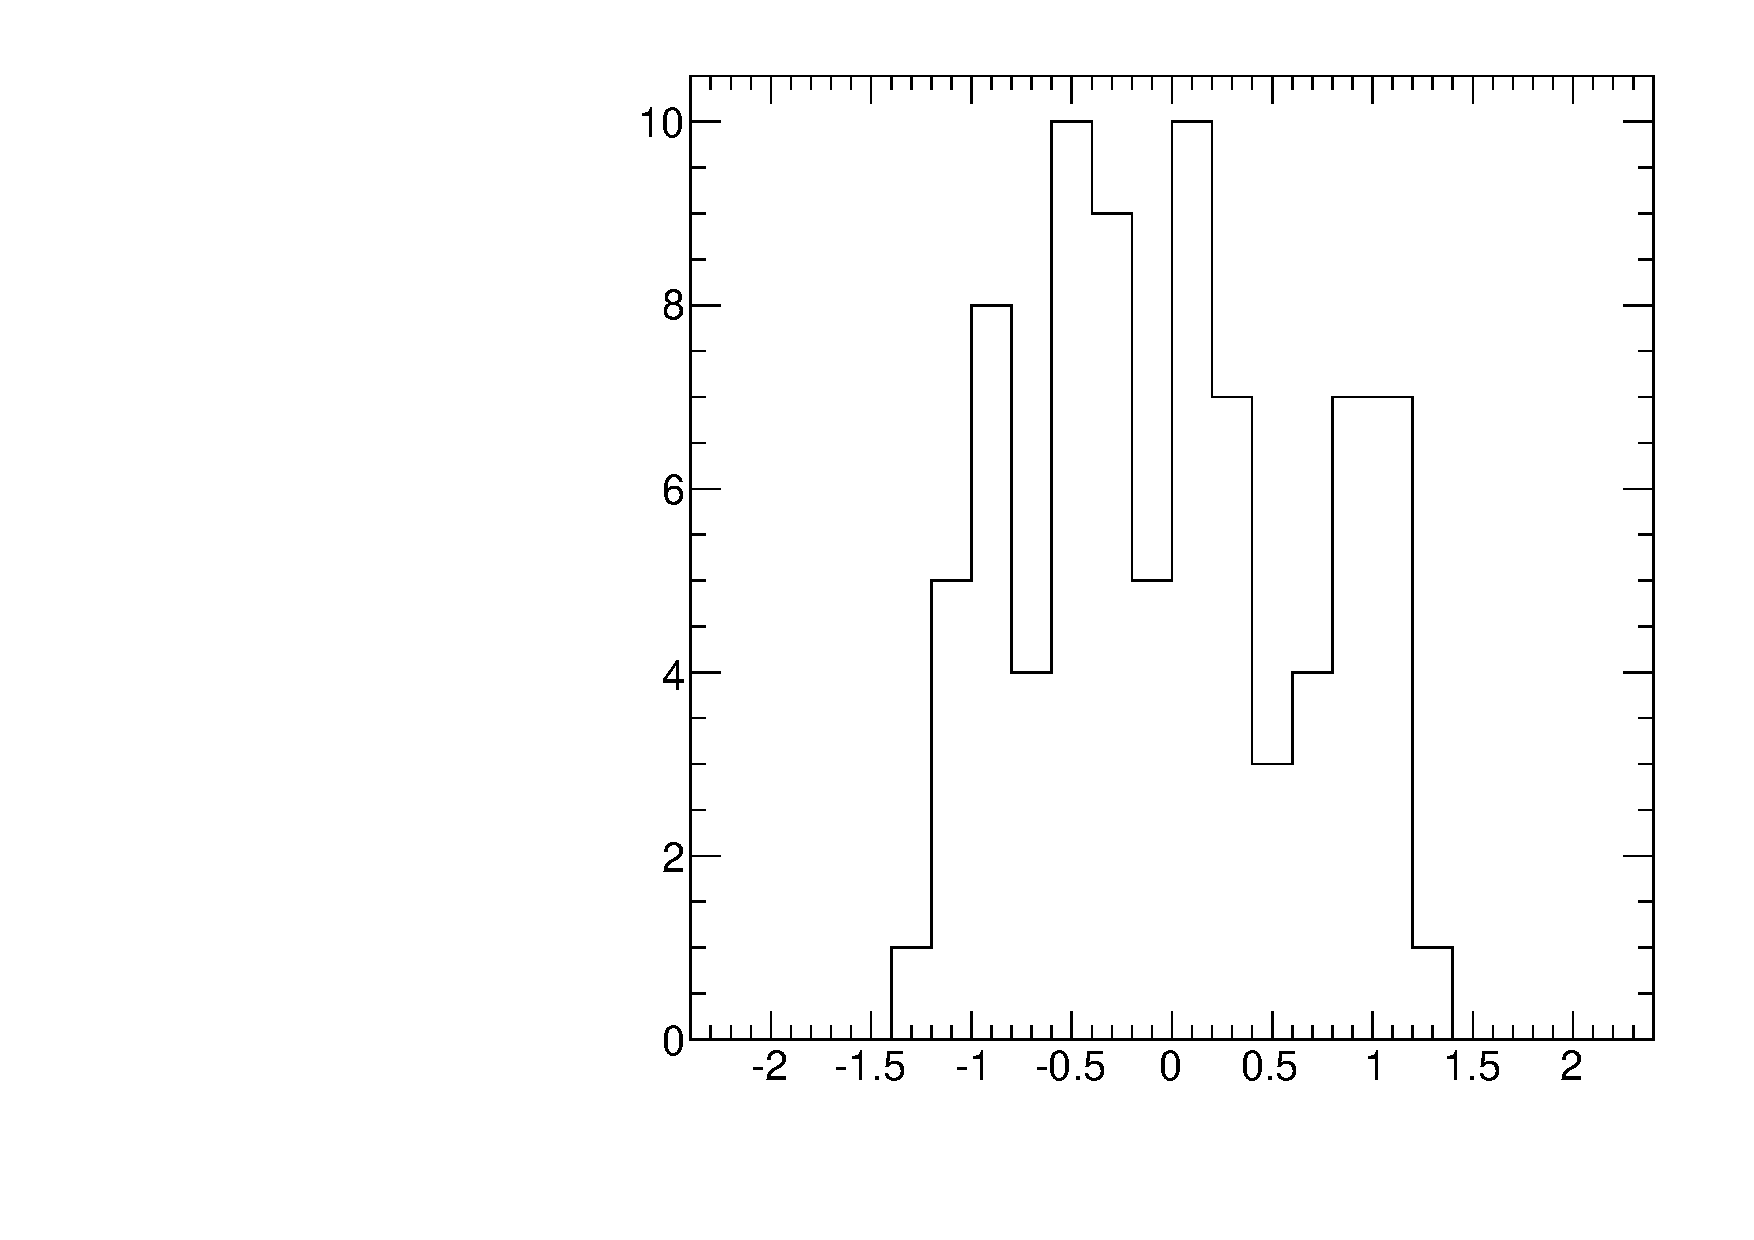
\includegraphics[width=0.3\textwidth]{Figures/AfterBDTCut_eta_BarrelUnblinded.pdf}
  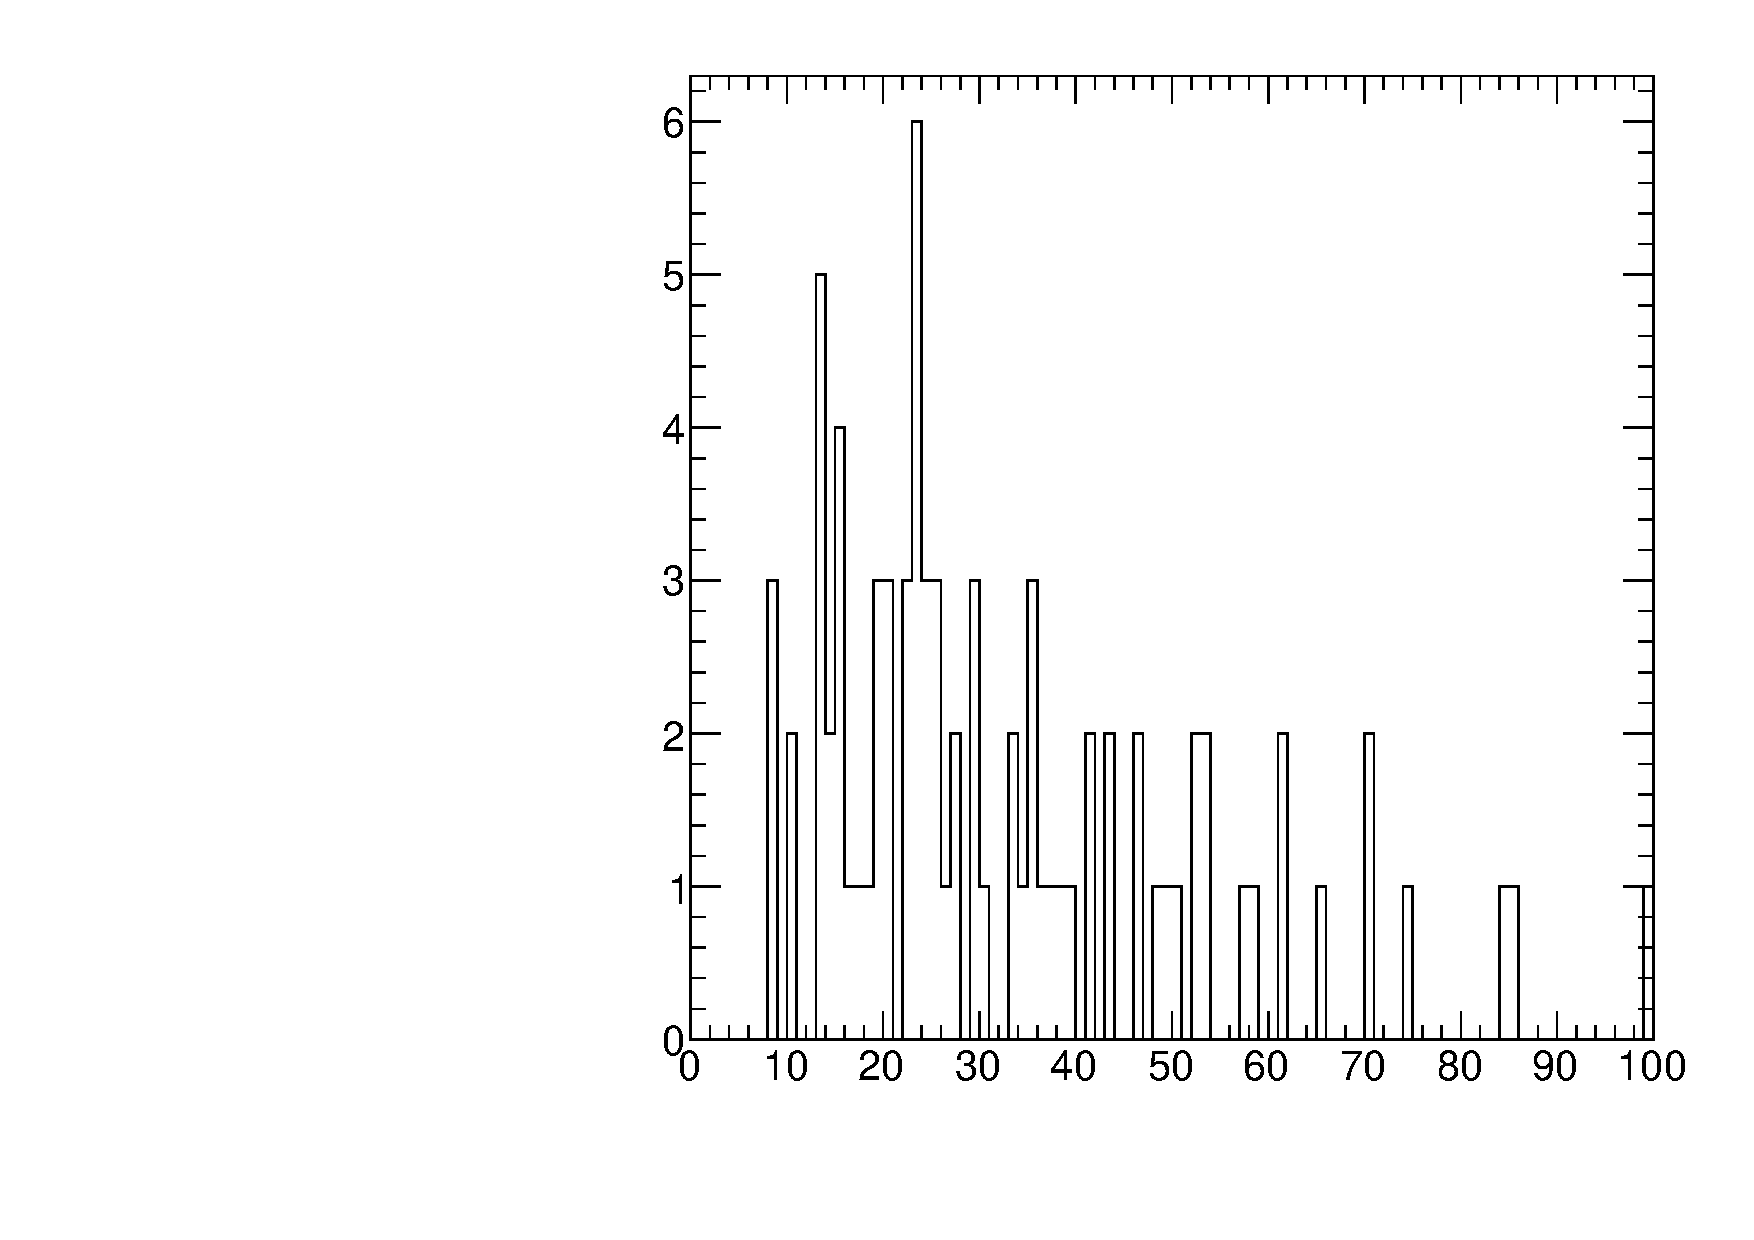
\includegraphics[width=0.3\textwidth]{Figures/AfterBDTCut_fls3d_BarrelUnblinded.pdf}
  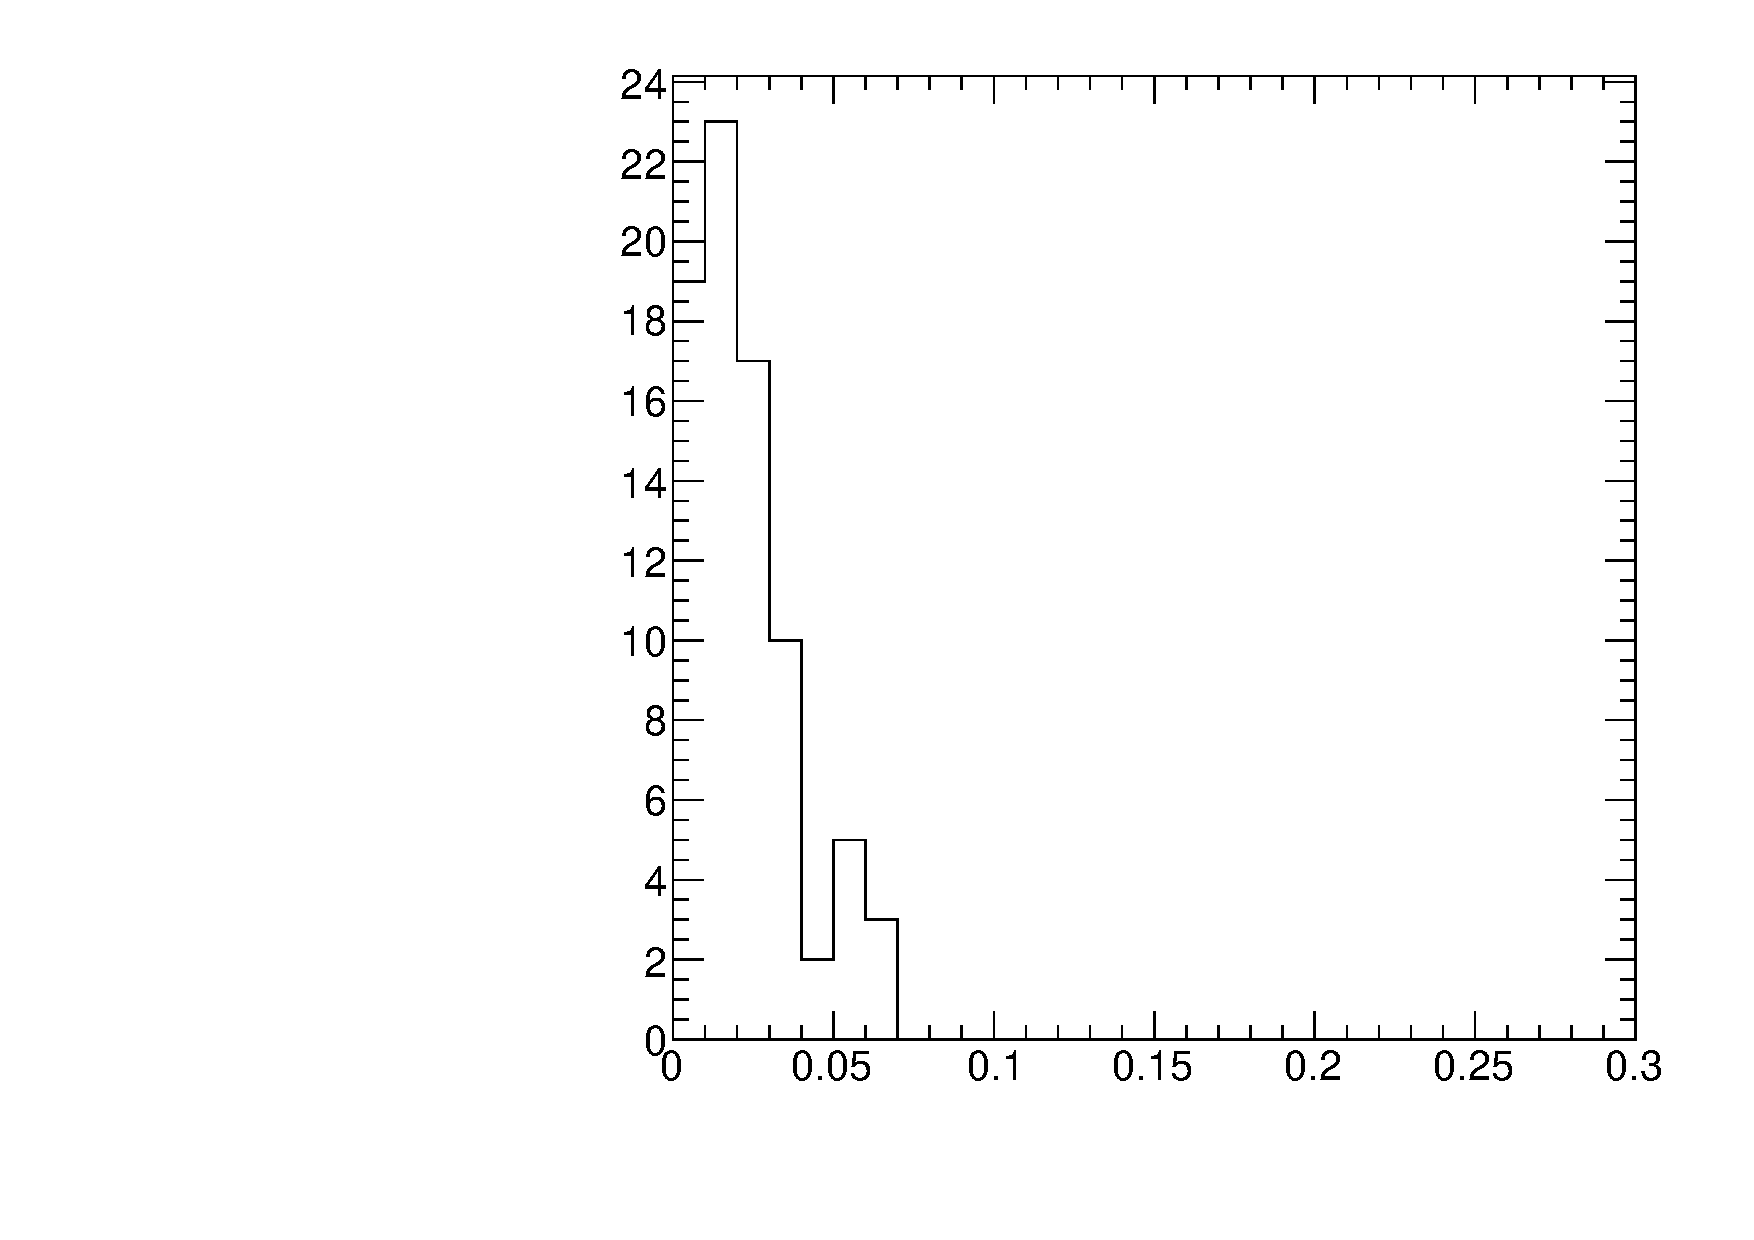
\includegraphics[width=0.3\textwidth]{Figures/AfterBDTCut_alpha_BarrelUnblinded.pdf}
  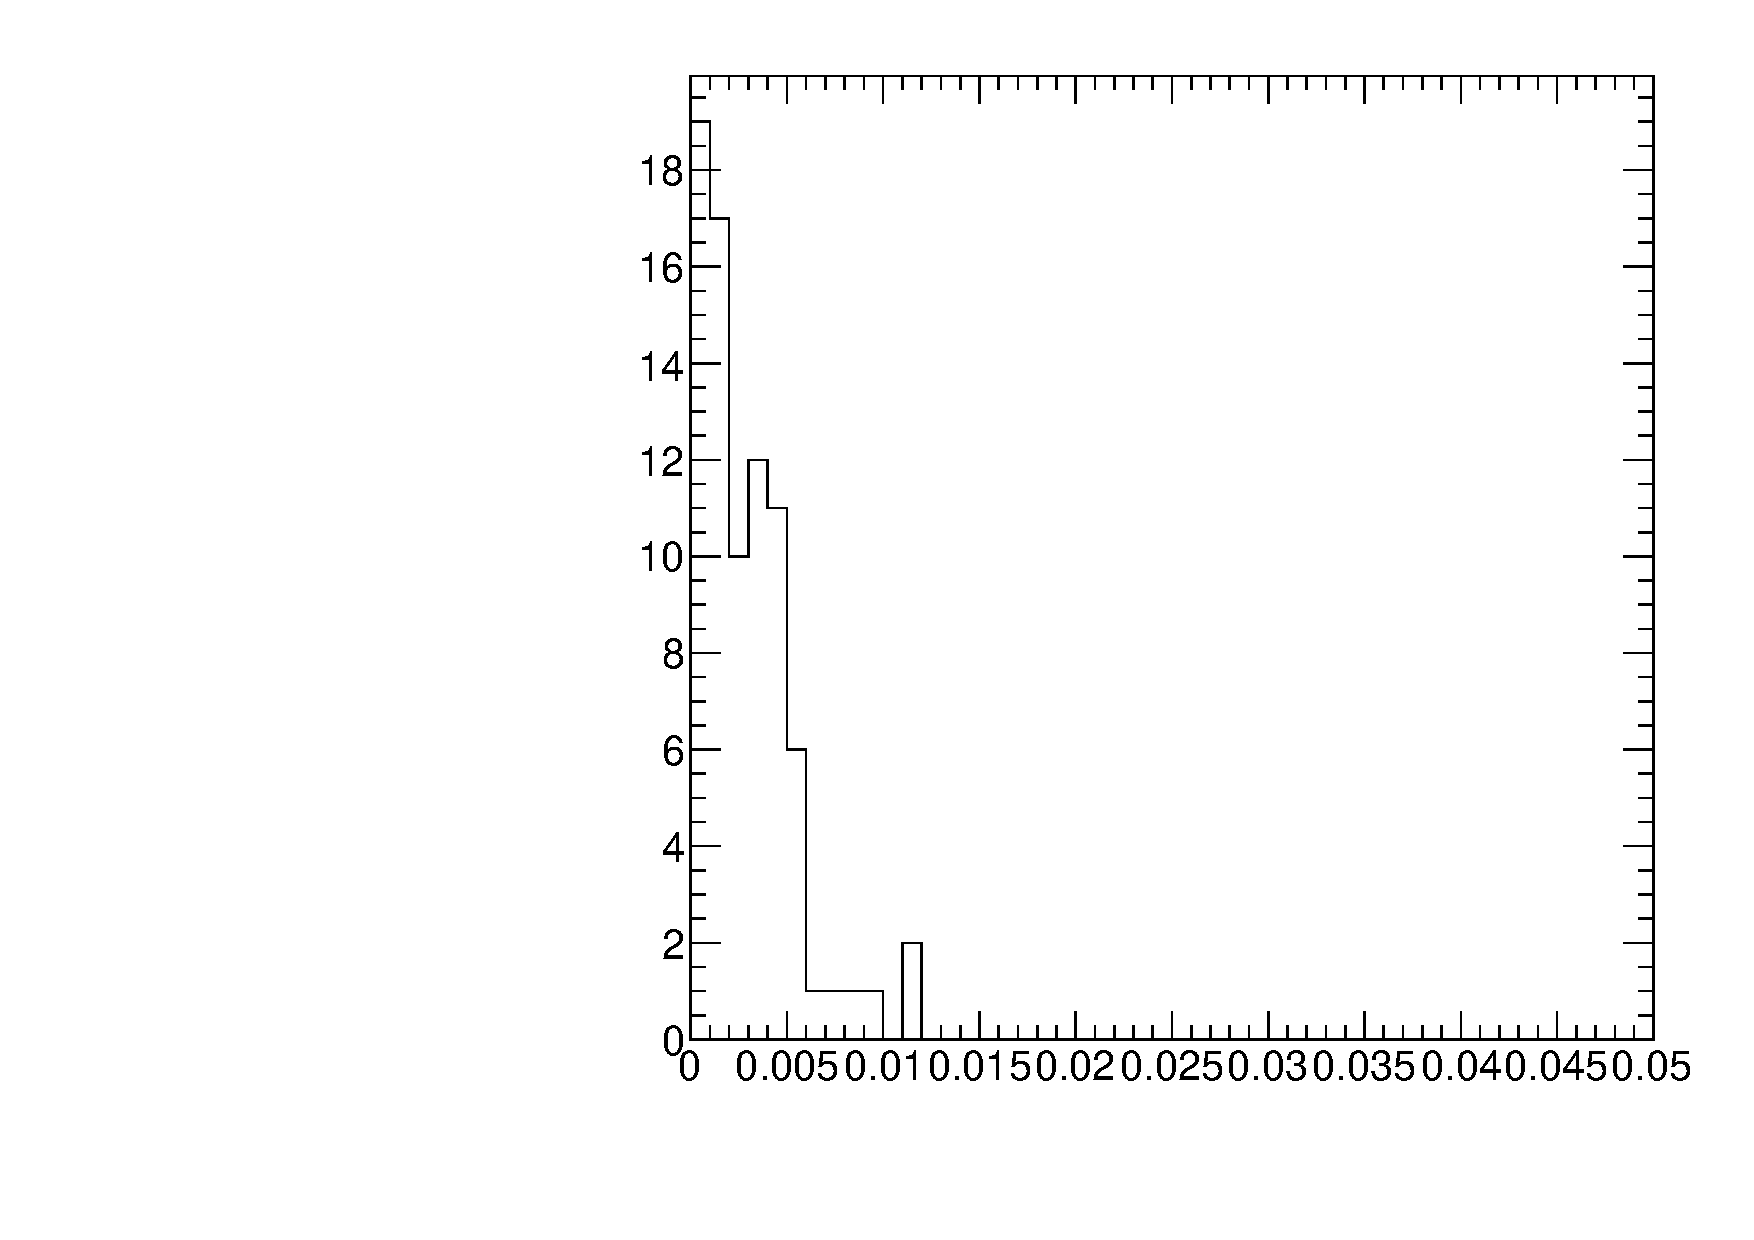
\includegraphics[width=0.3\textwidth]{Figures/AfterBDTCut_maxdoca_BarrelUnblinded.pdf}
  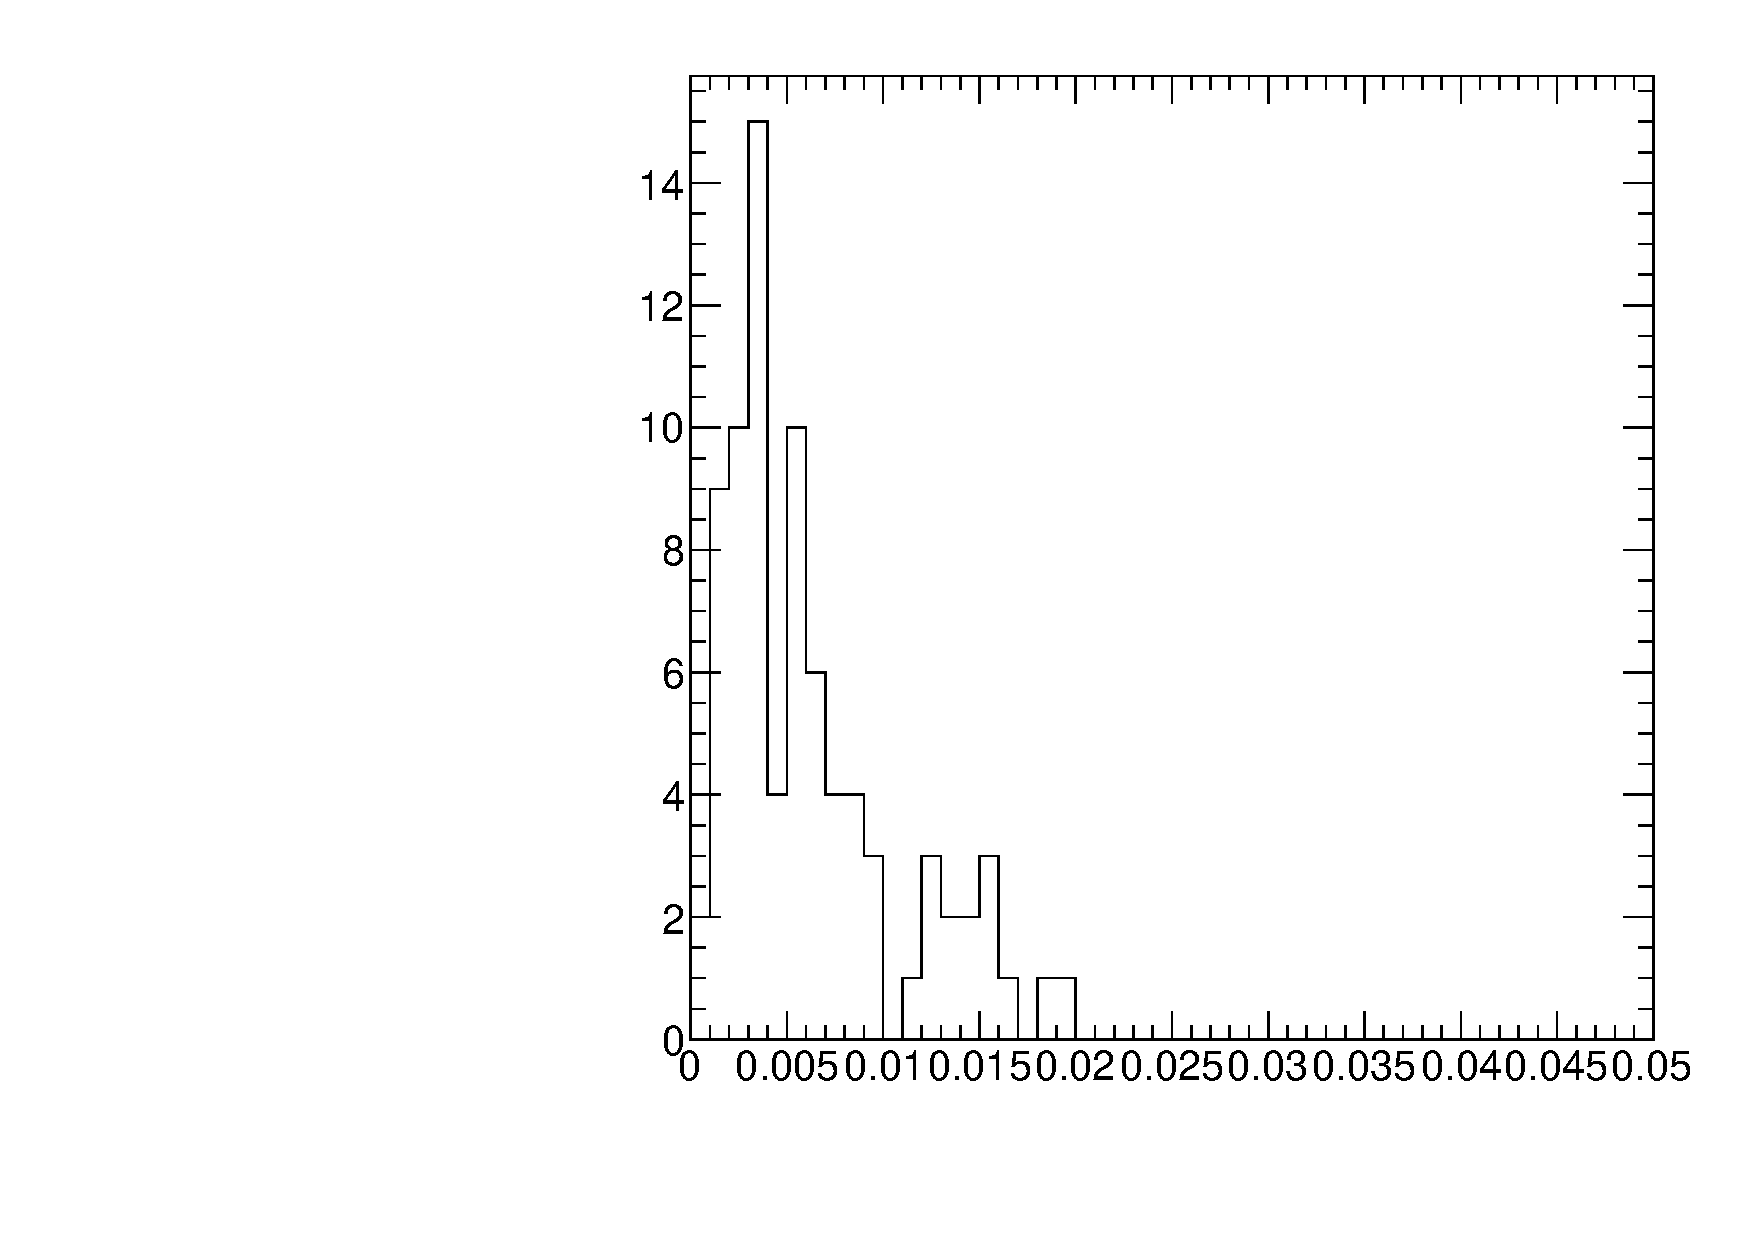
\includegraphics[width=0.3\textwidth]{Figures/AfterBDTCut_pvip_BarrelUnblinded.pdf}
  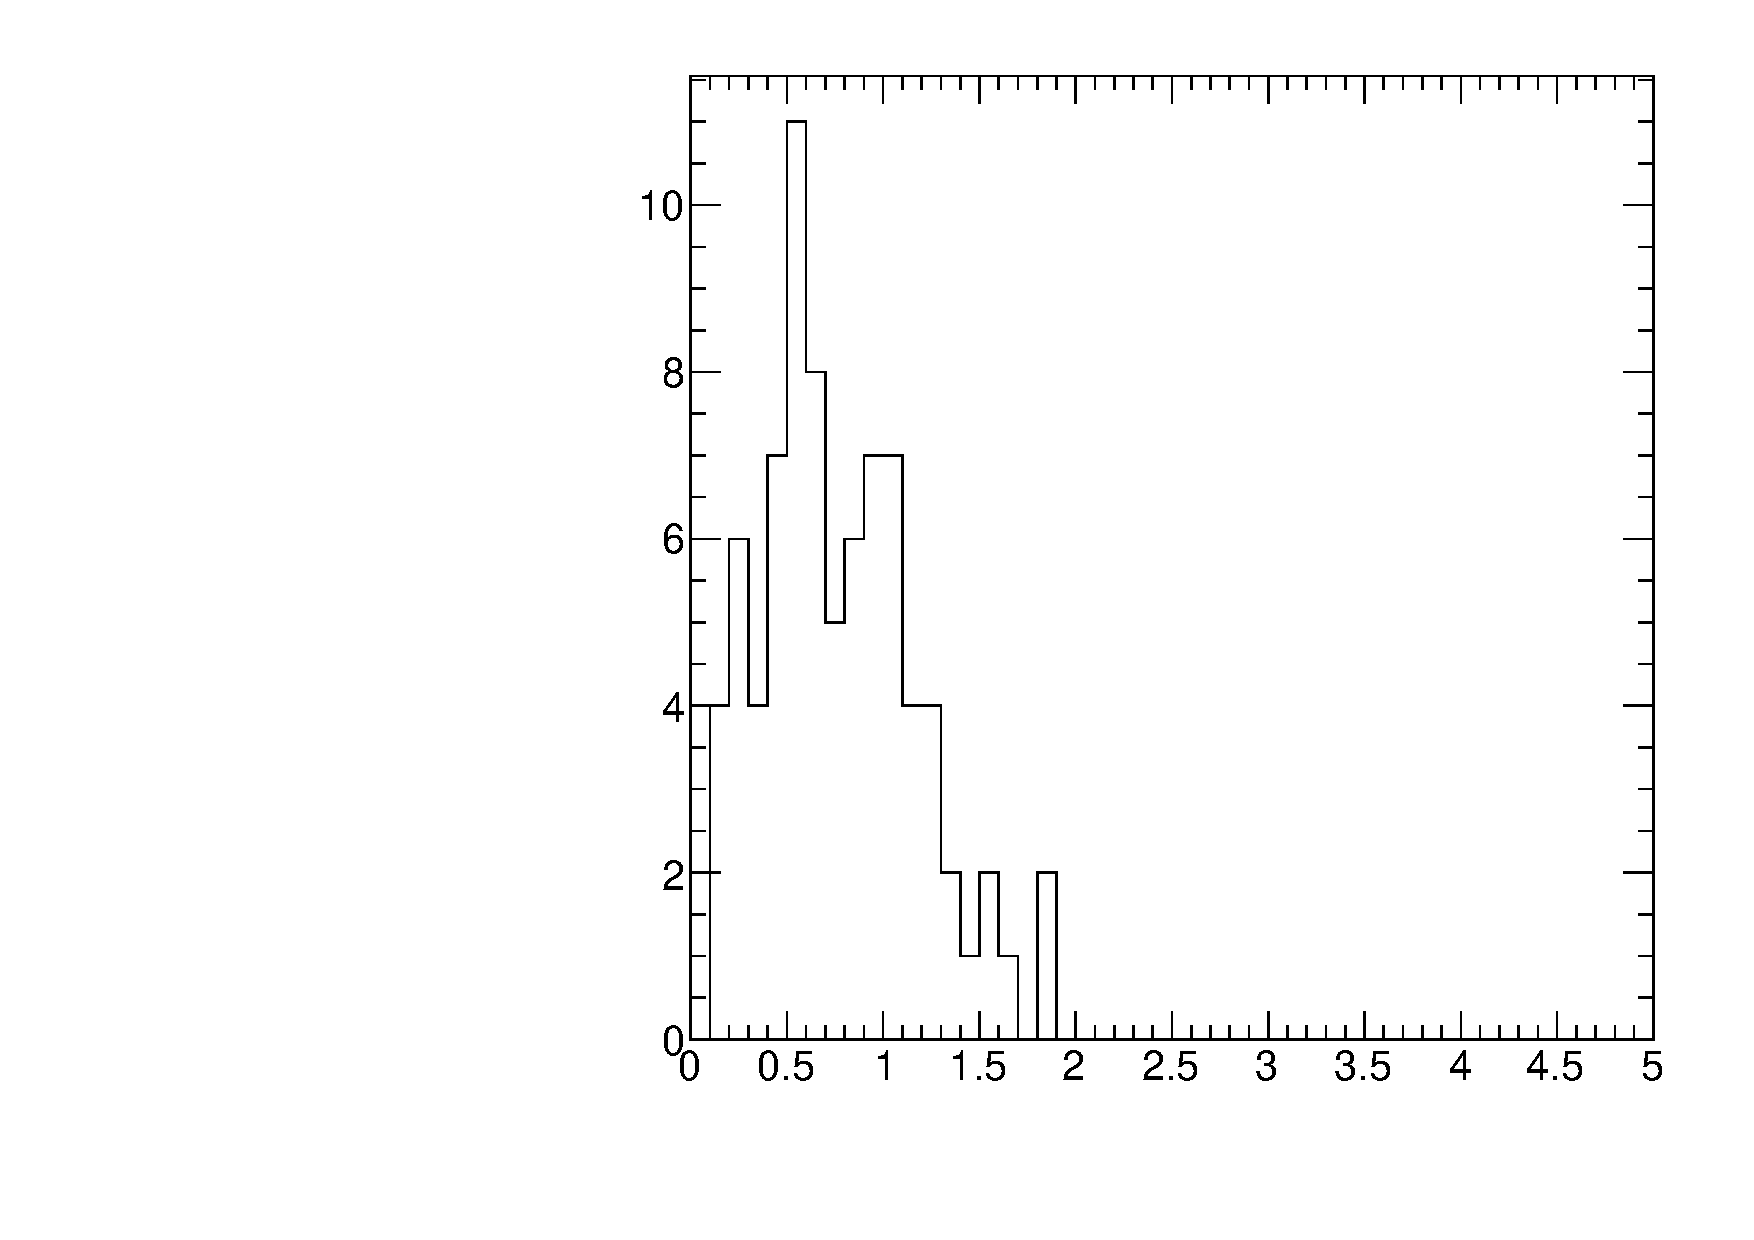
\includegraphics[width=0.3\textwidth]{Figures/AfterBDTCut_pvips_BarrelUnblinded.pdf}
  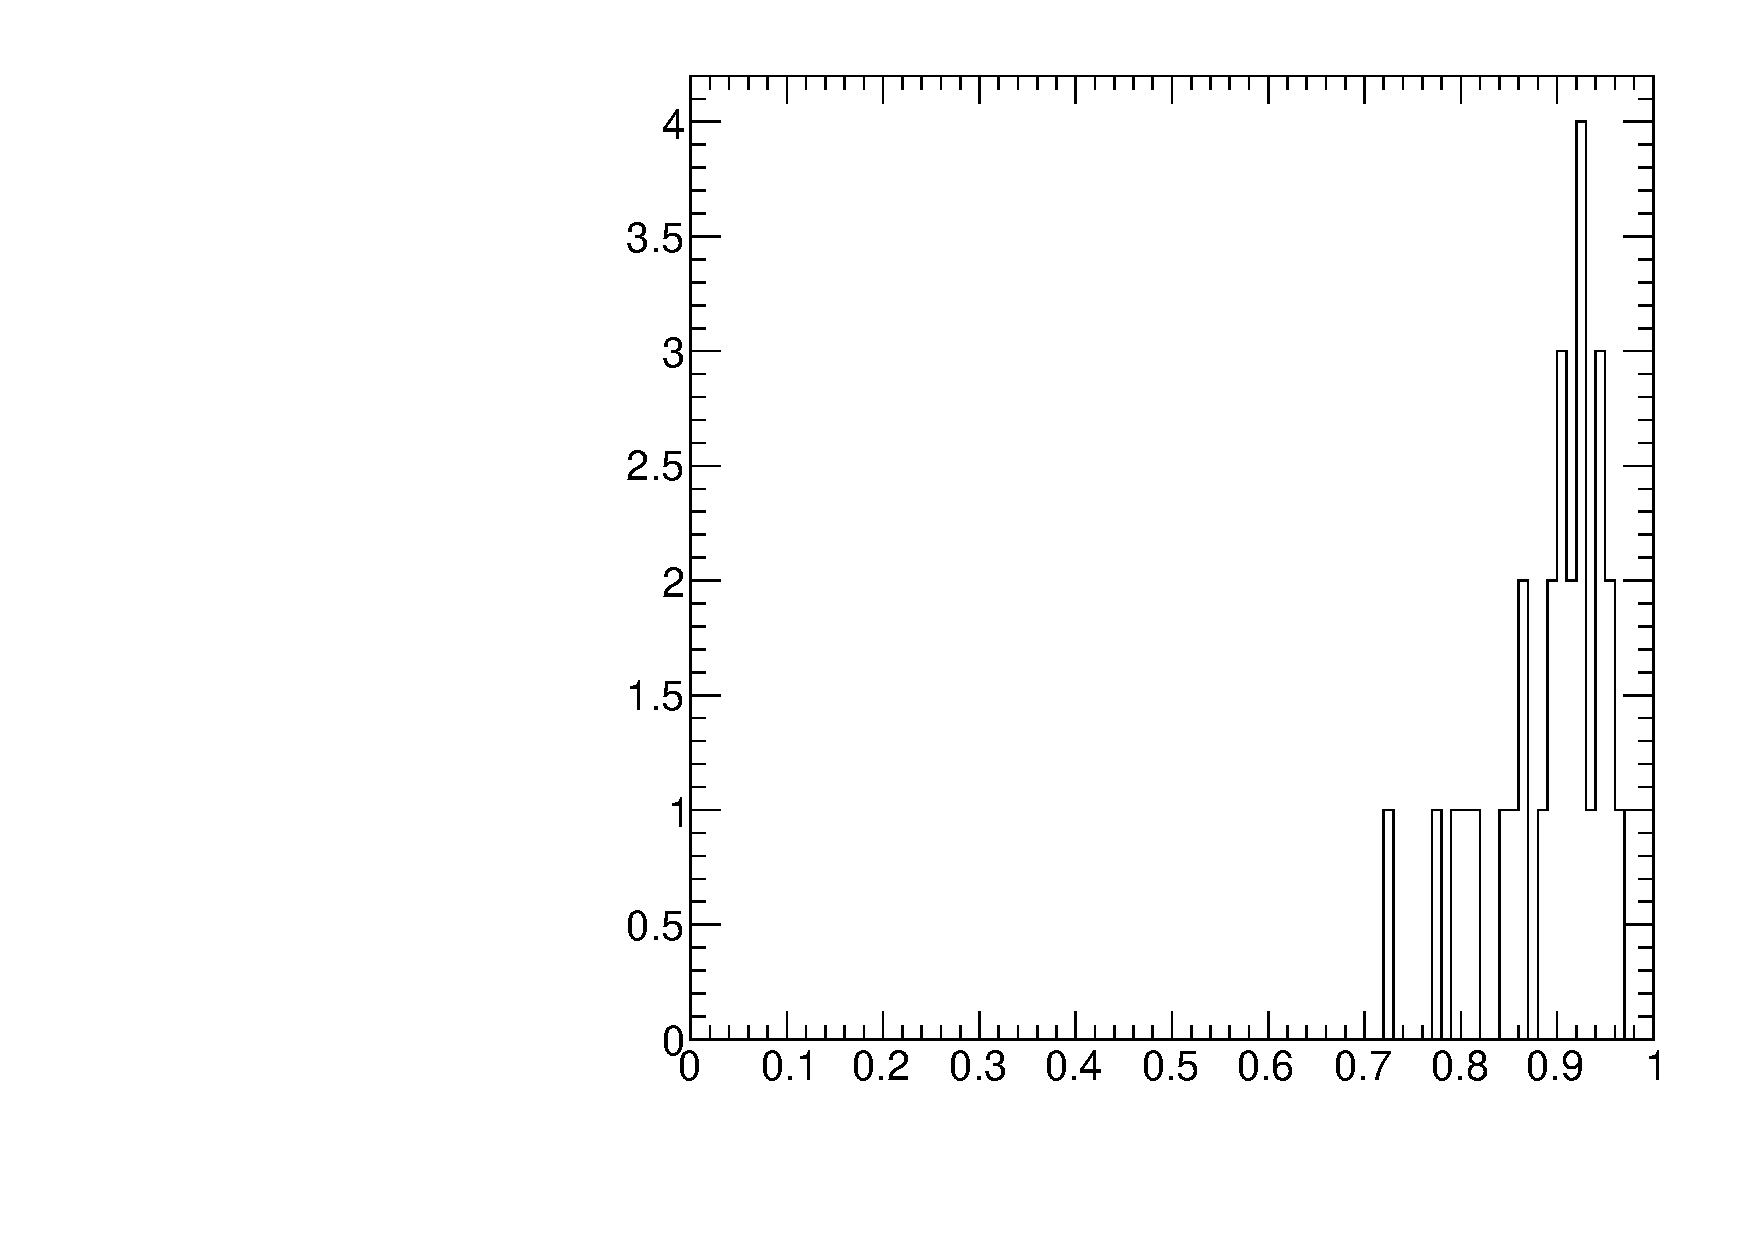
\includegraphics[width=0.3\textwidth]{Figures/AfterBDTCut_iso_BarrelUnblinded.pdf}
  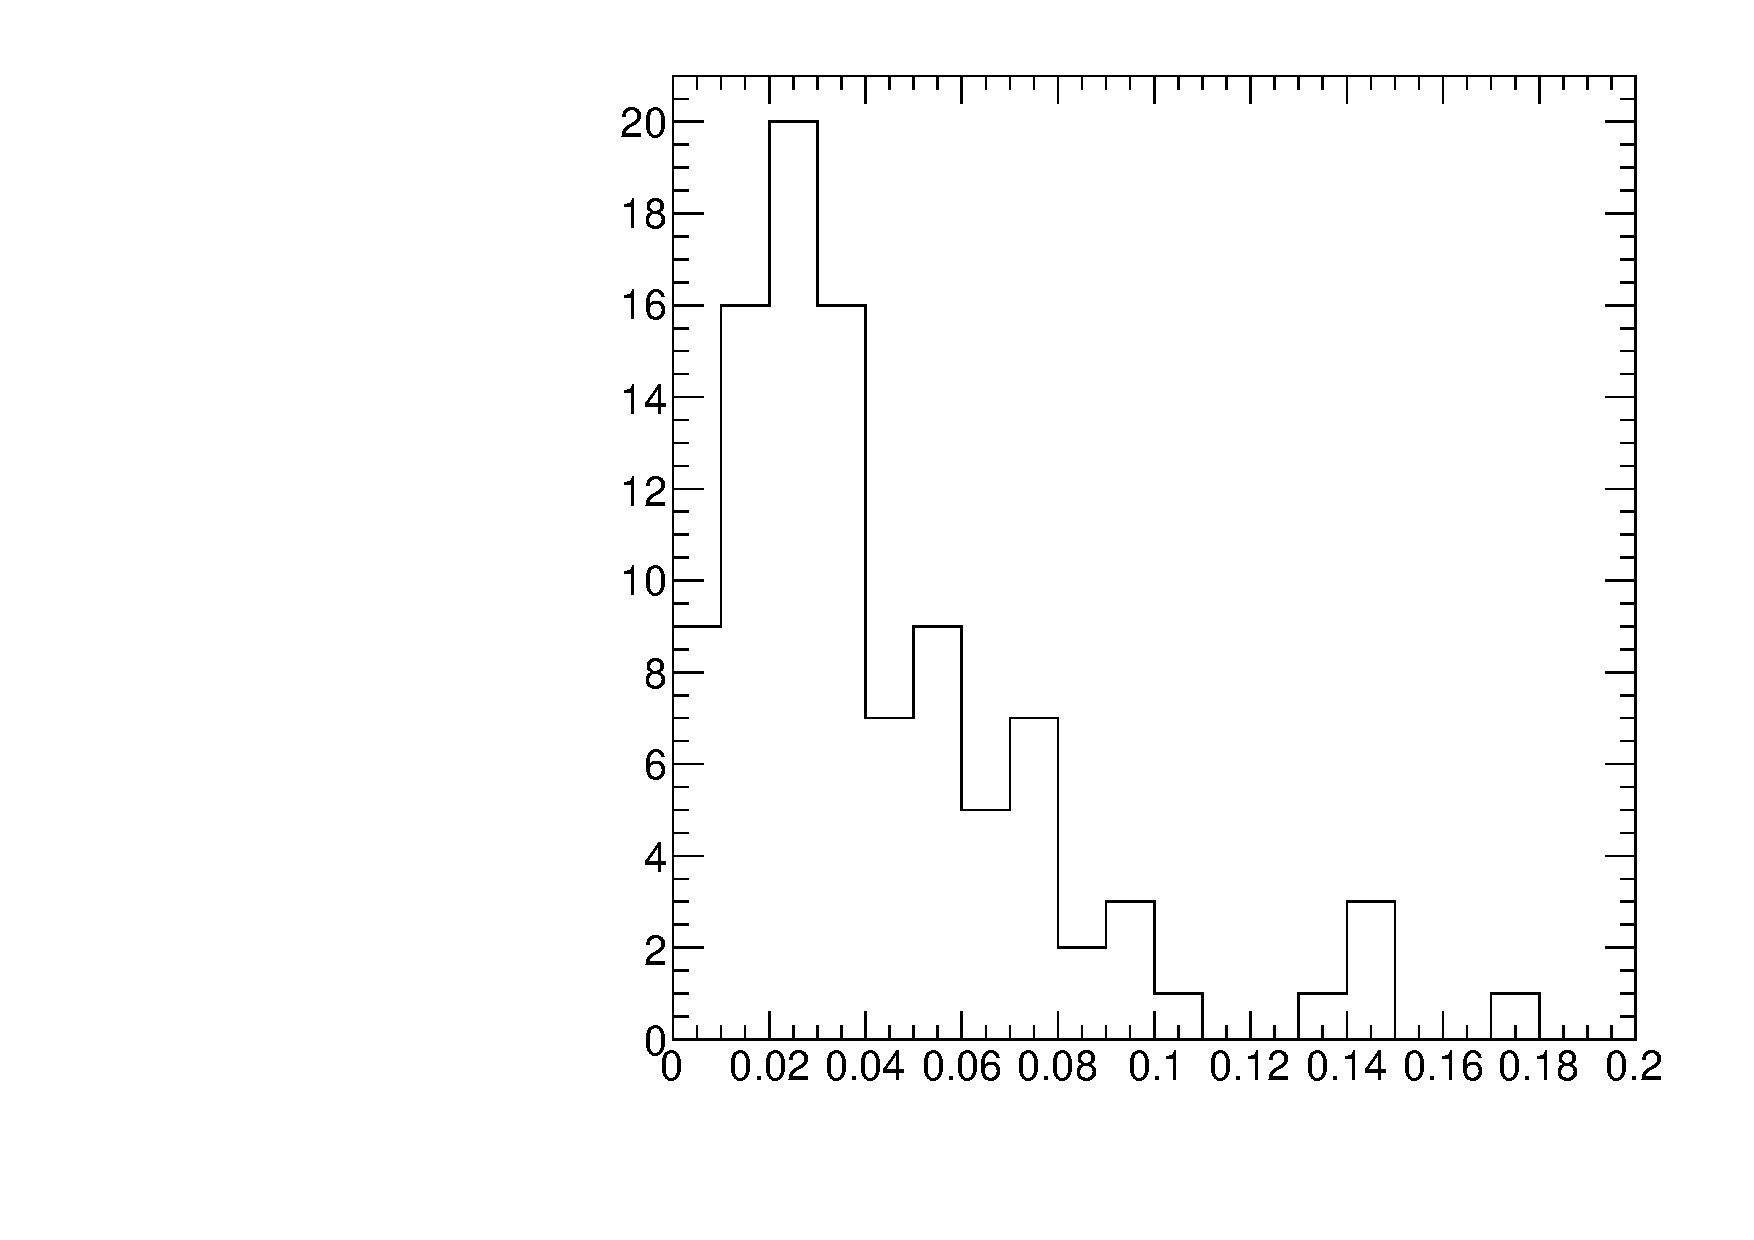
\includegraphics[width=0.3\textwidth]{Figures/AfterBDTCut_docatrk_BarrelUnblinded.pdf}
  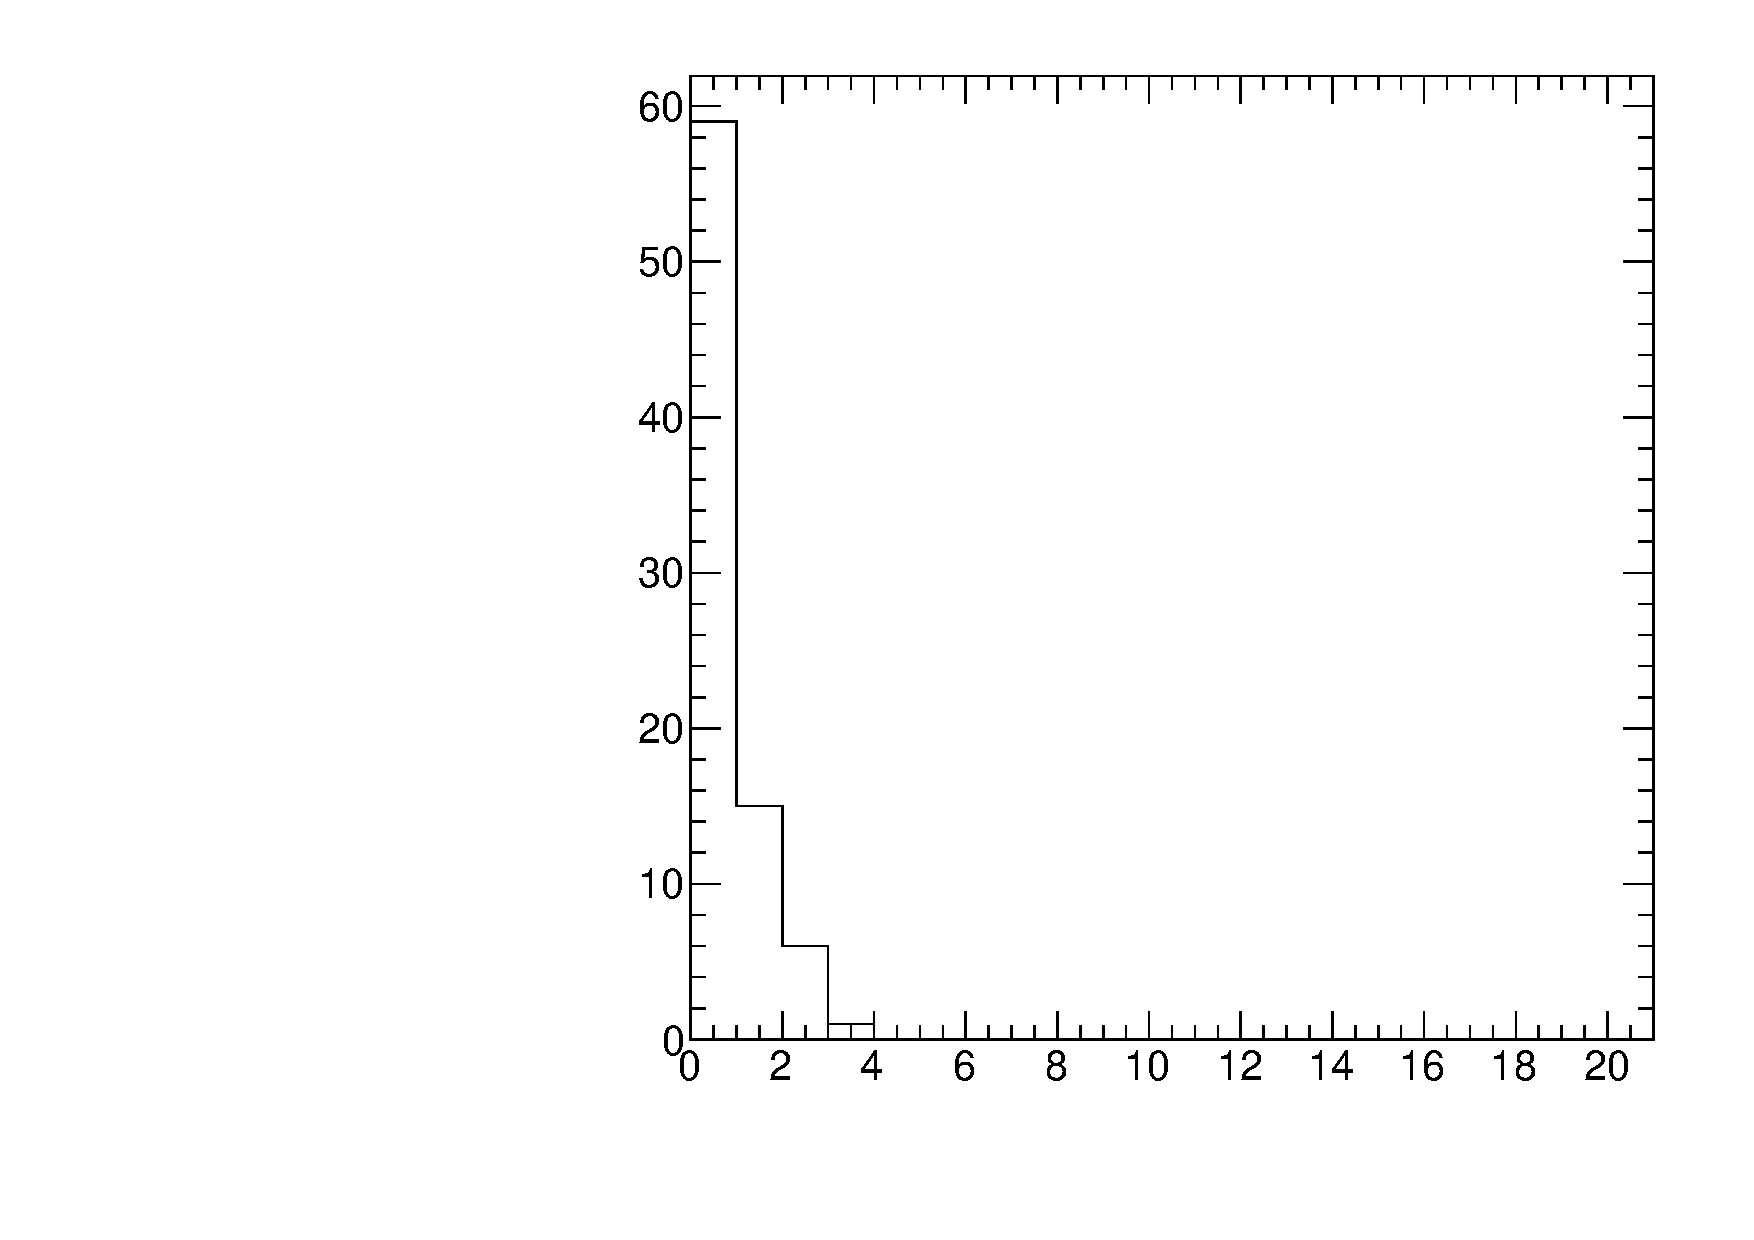
\includegraphics[width=0.3\textwidth]{Figures/AfterBDTCut_closetrk_BarrelUnblinded.pdf}
  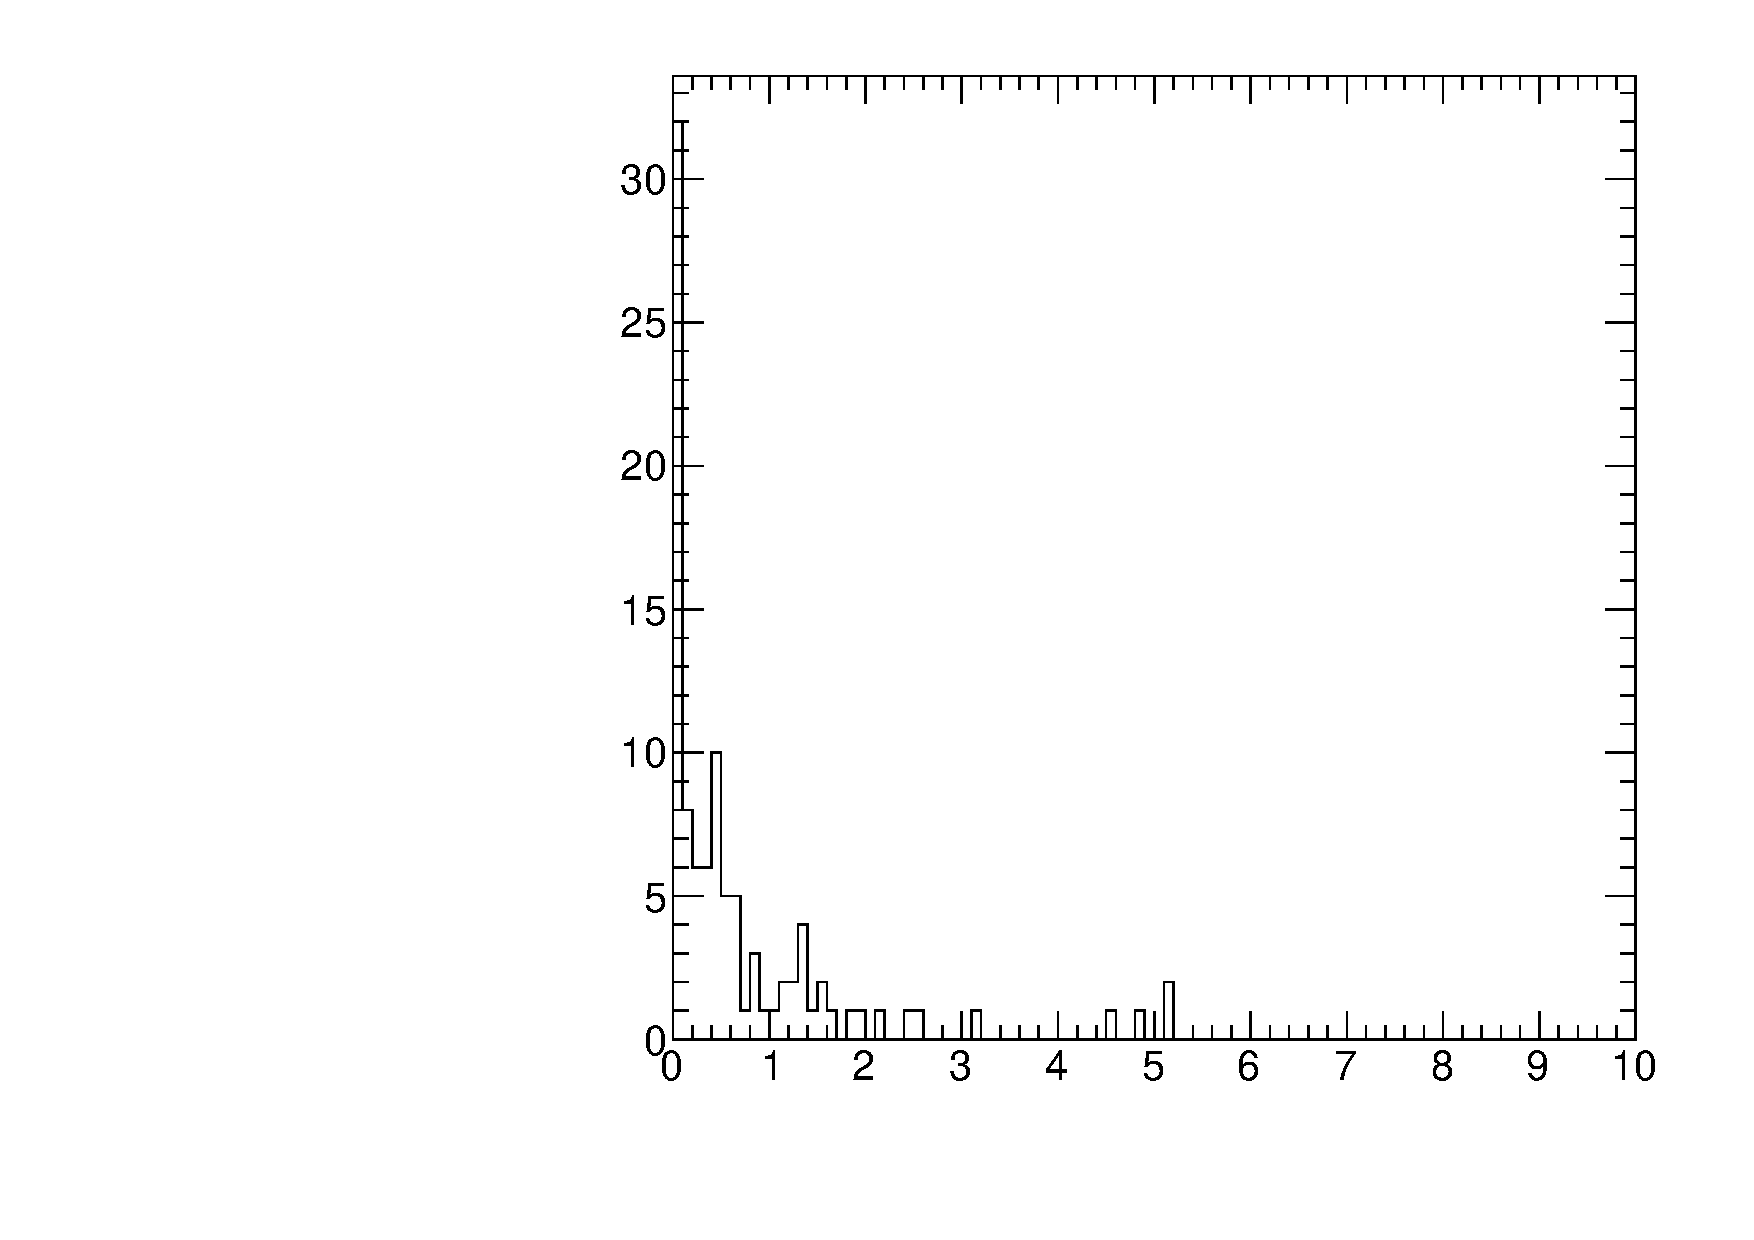
\includegraphics[width=0.3\textwidth]{Figures/AfterBDTCut_chi2dof_BarrelUnblinded.pdf}
  \caption{Variable distributions for the barrel after BDT cuts on unblinded data.}
  \label{fig:AfterBDTCutVariablesBarrelUnblinded}
\end{figure}

\begin{figure}
  \centering
  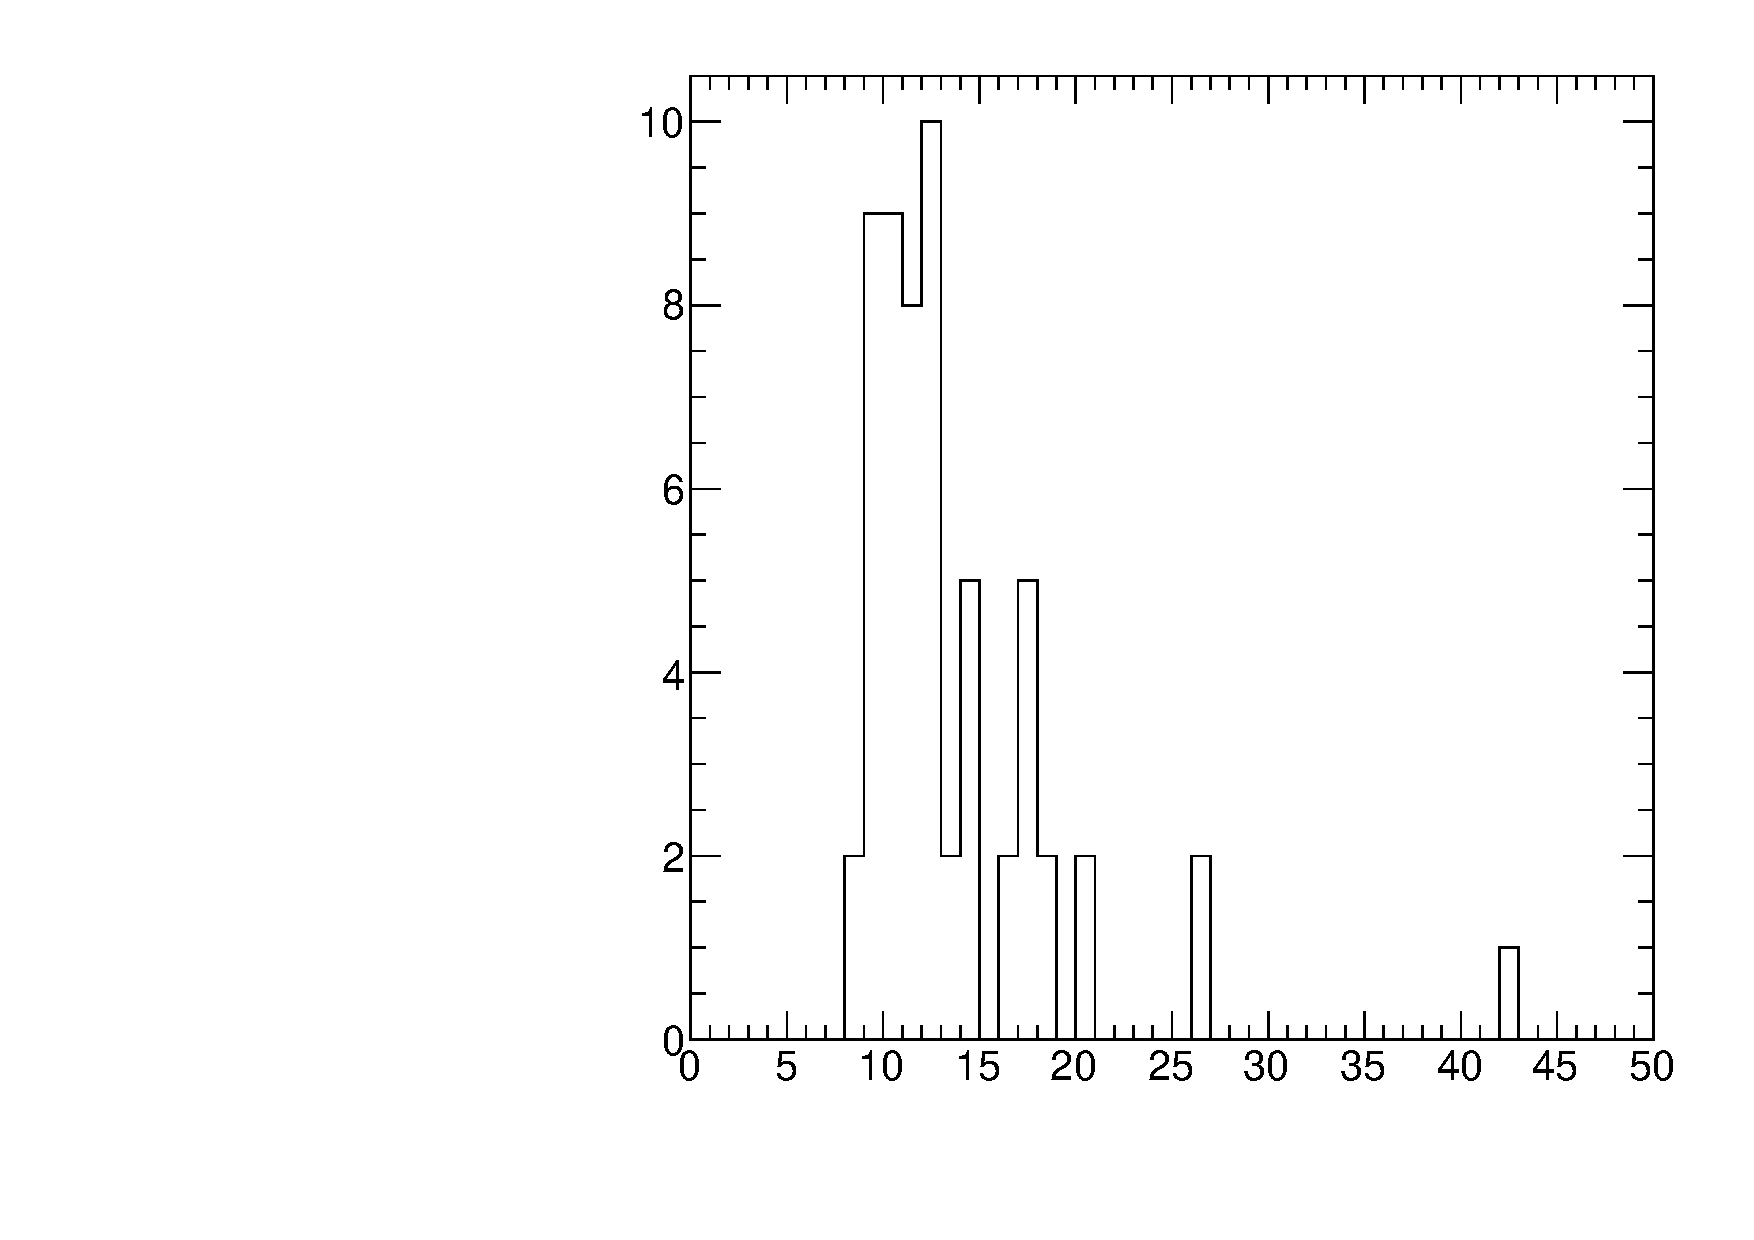
\includegraphics[width=0.3\textwidth]{Figures/AfterBDTCut_pt_EndcapsUnblinded.pdf}
  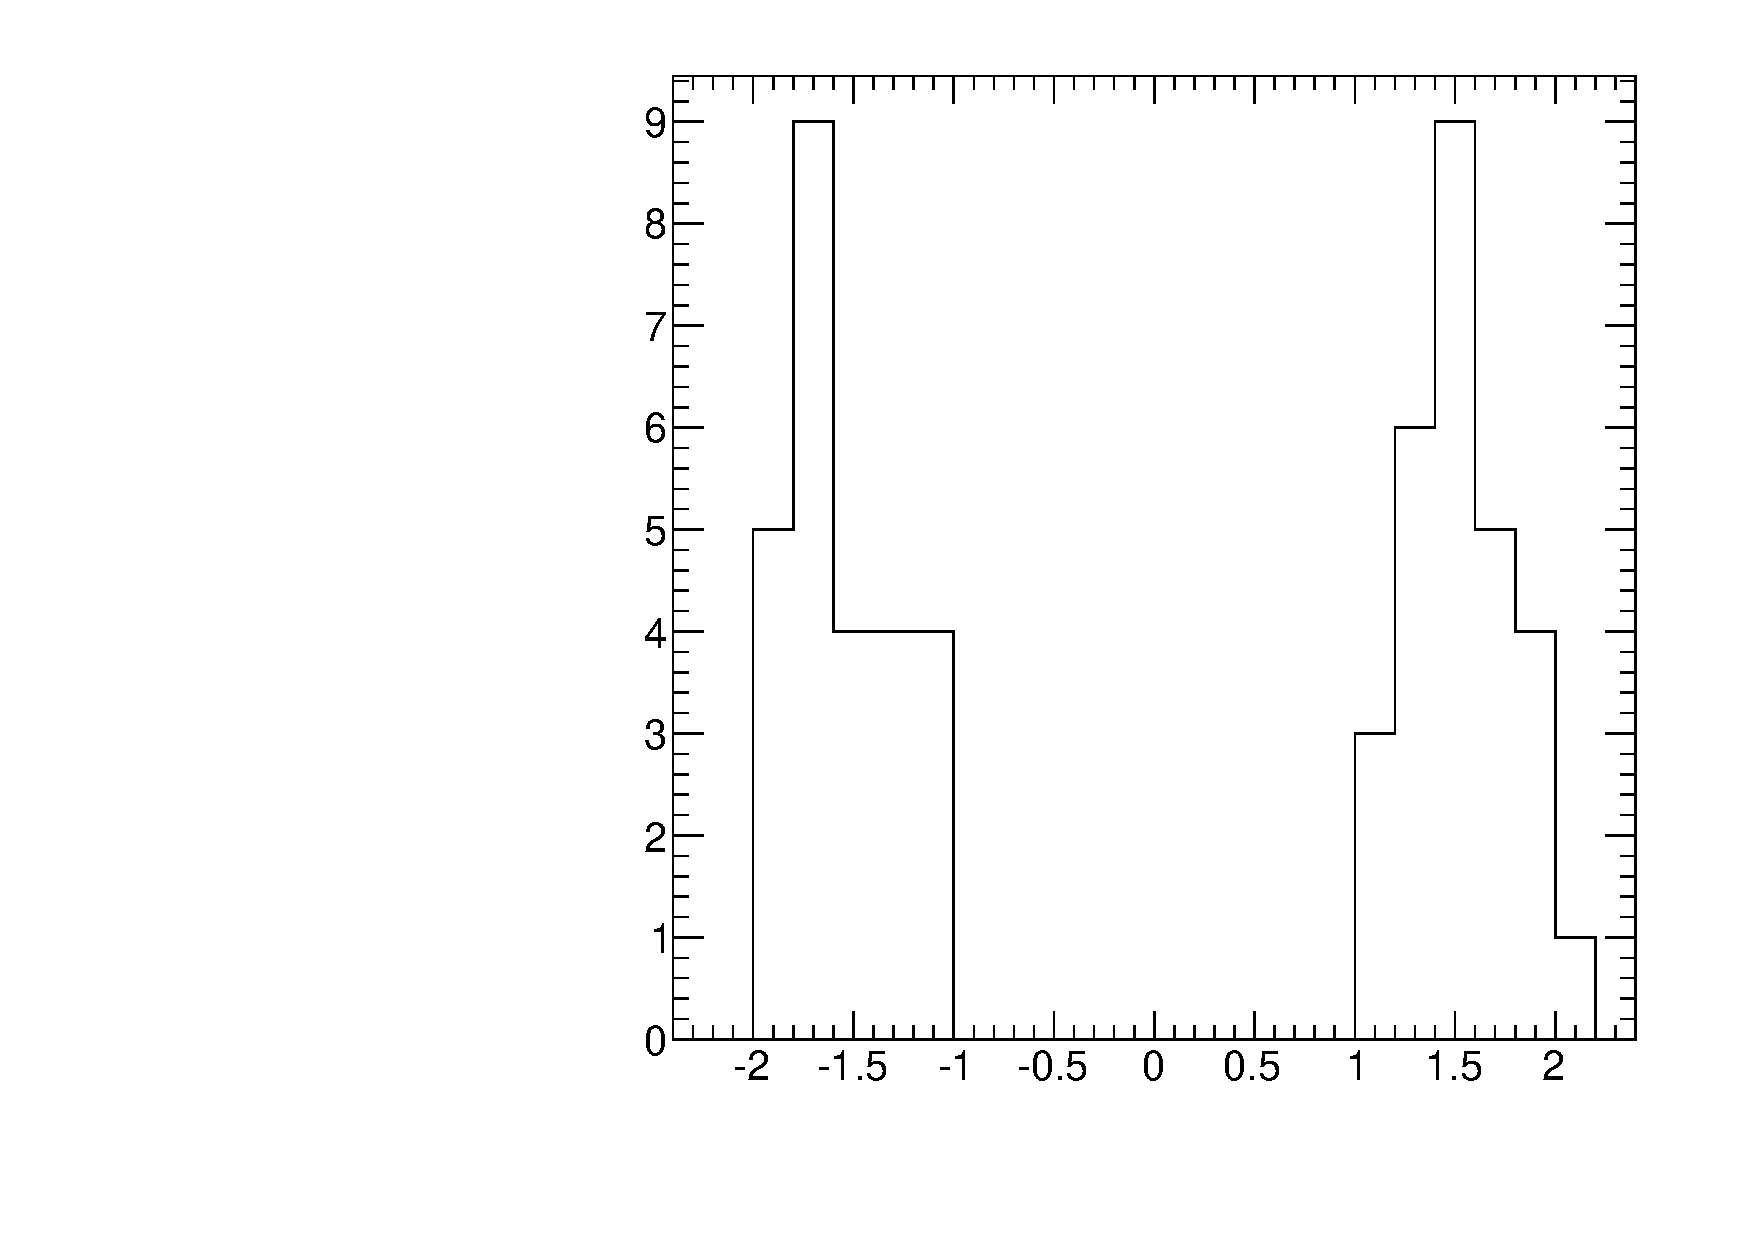
\includegraphics[width=0.3\textwidth]{Figures/AfterBDTCut_eta_EndcapsUnblinded.pdf}
  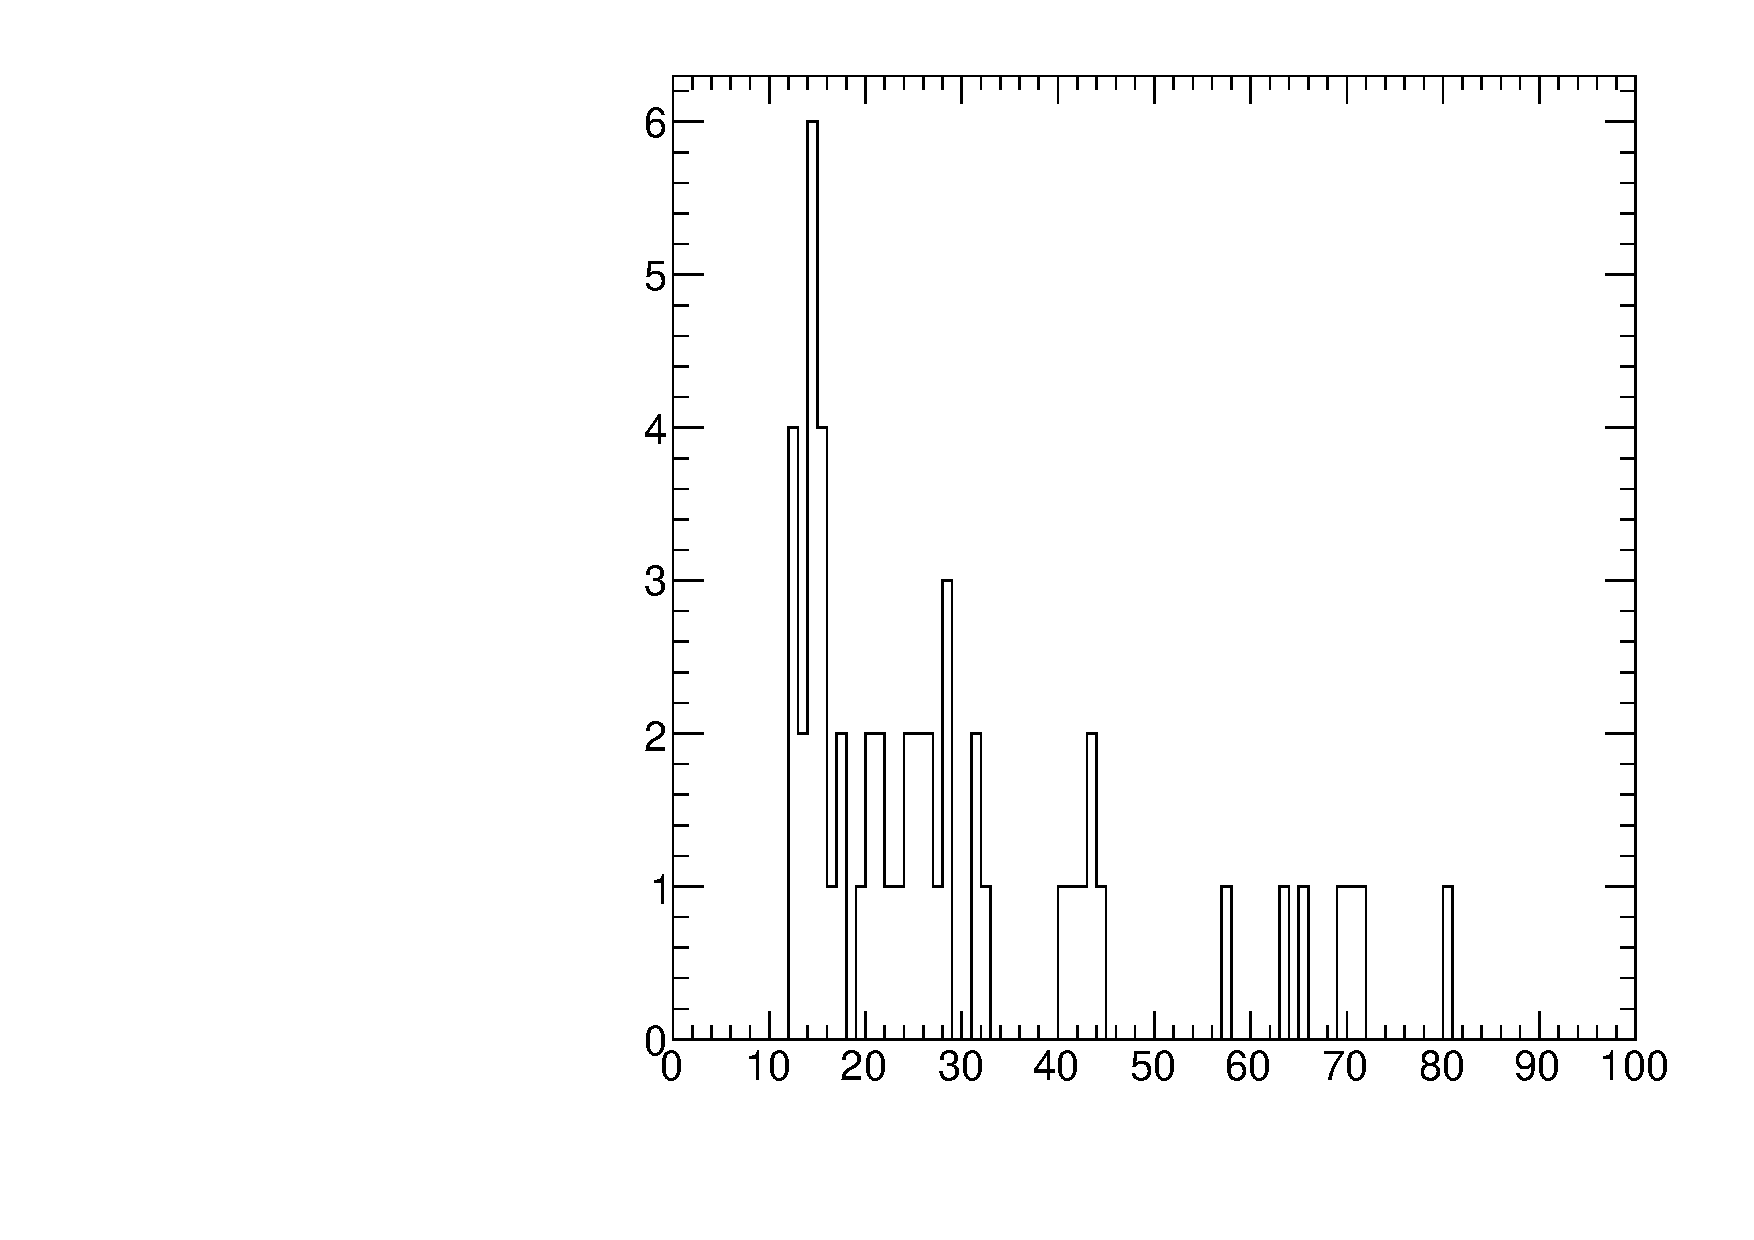
\includegraphics[width=0.3\textwidth]{Figures/AfterBDTCut_fls3d_EndcapsUnblinded.pdf}
  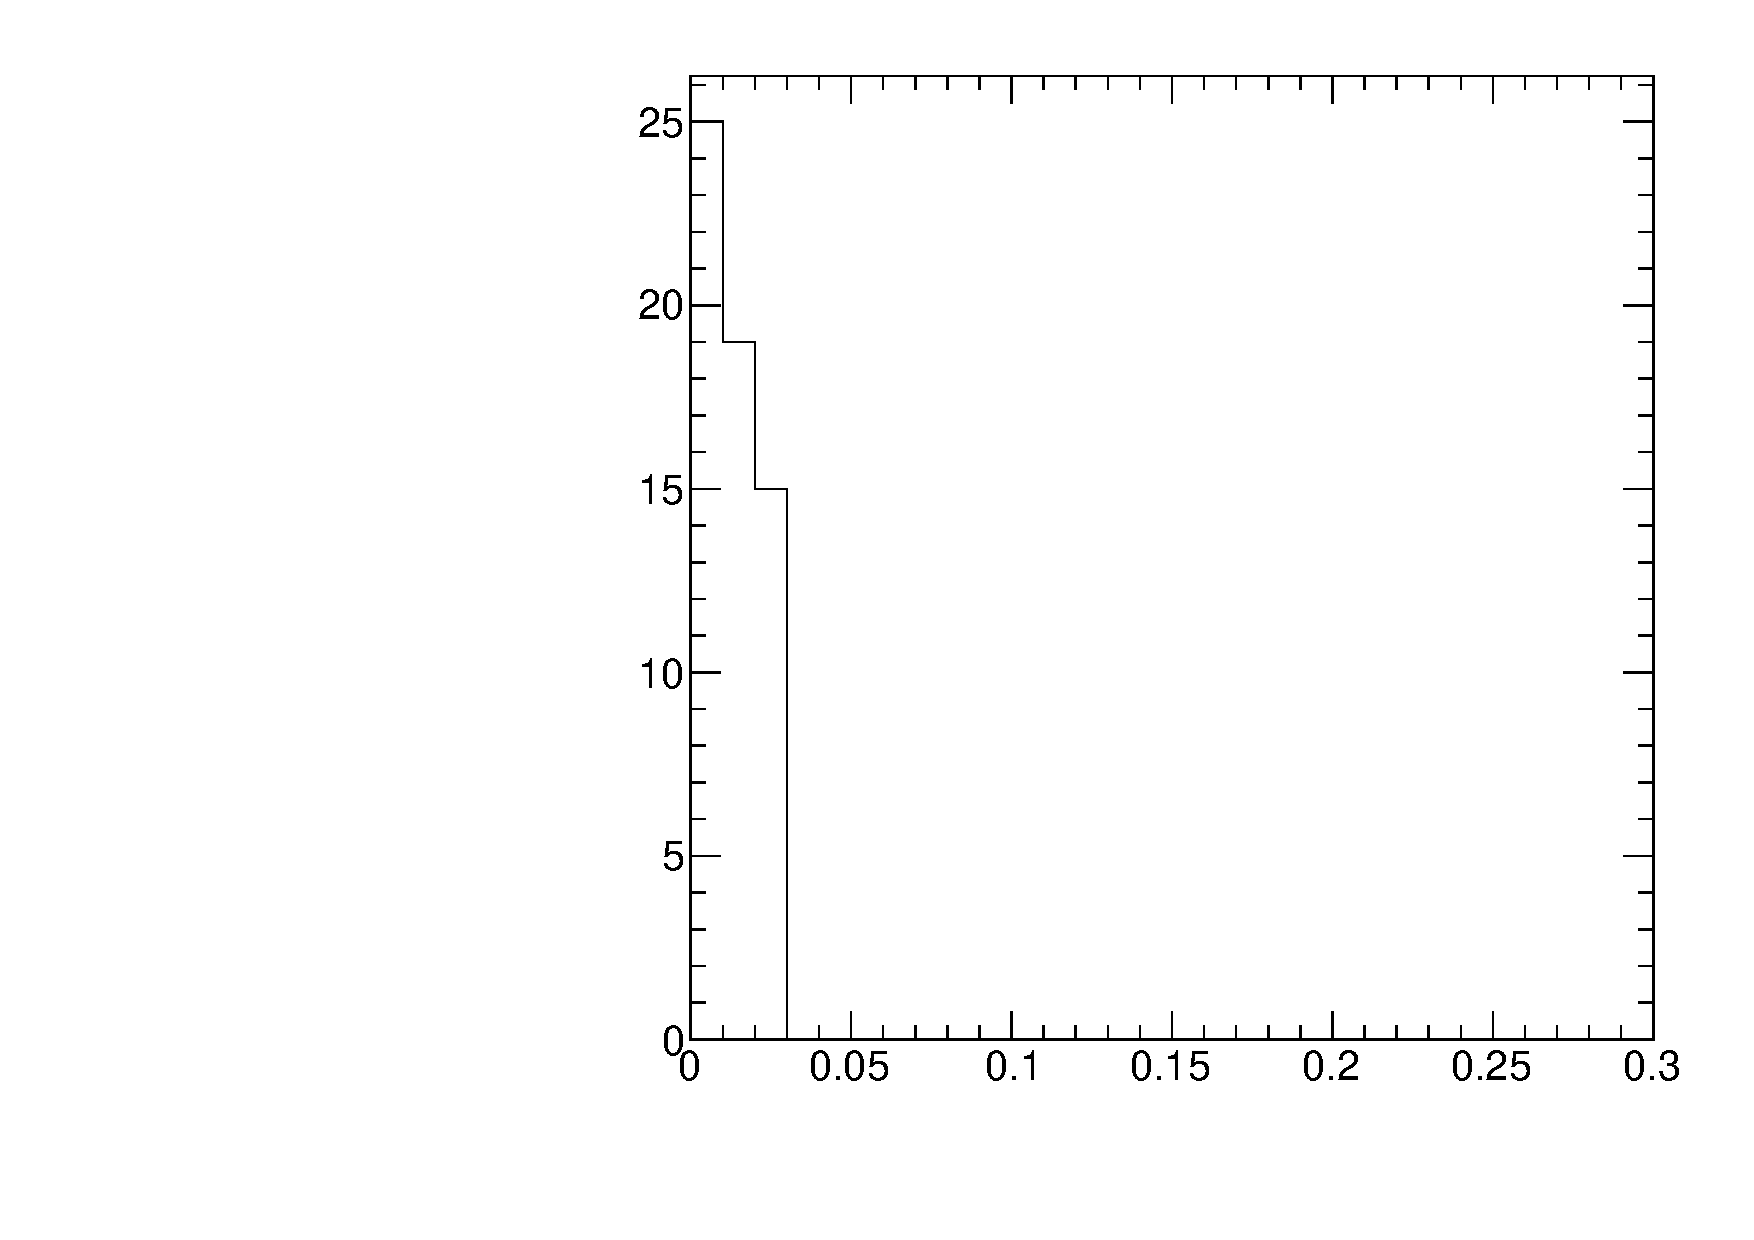
\includegraphics[width=0.3\textwidth]{Figures/AfterBDTCut_alpha_EndcapsUnblinded.pdf}
  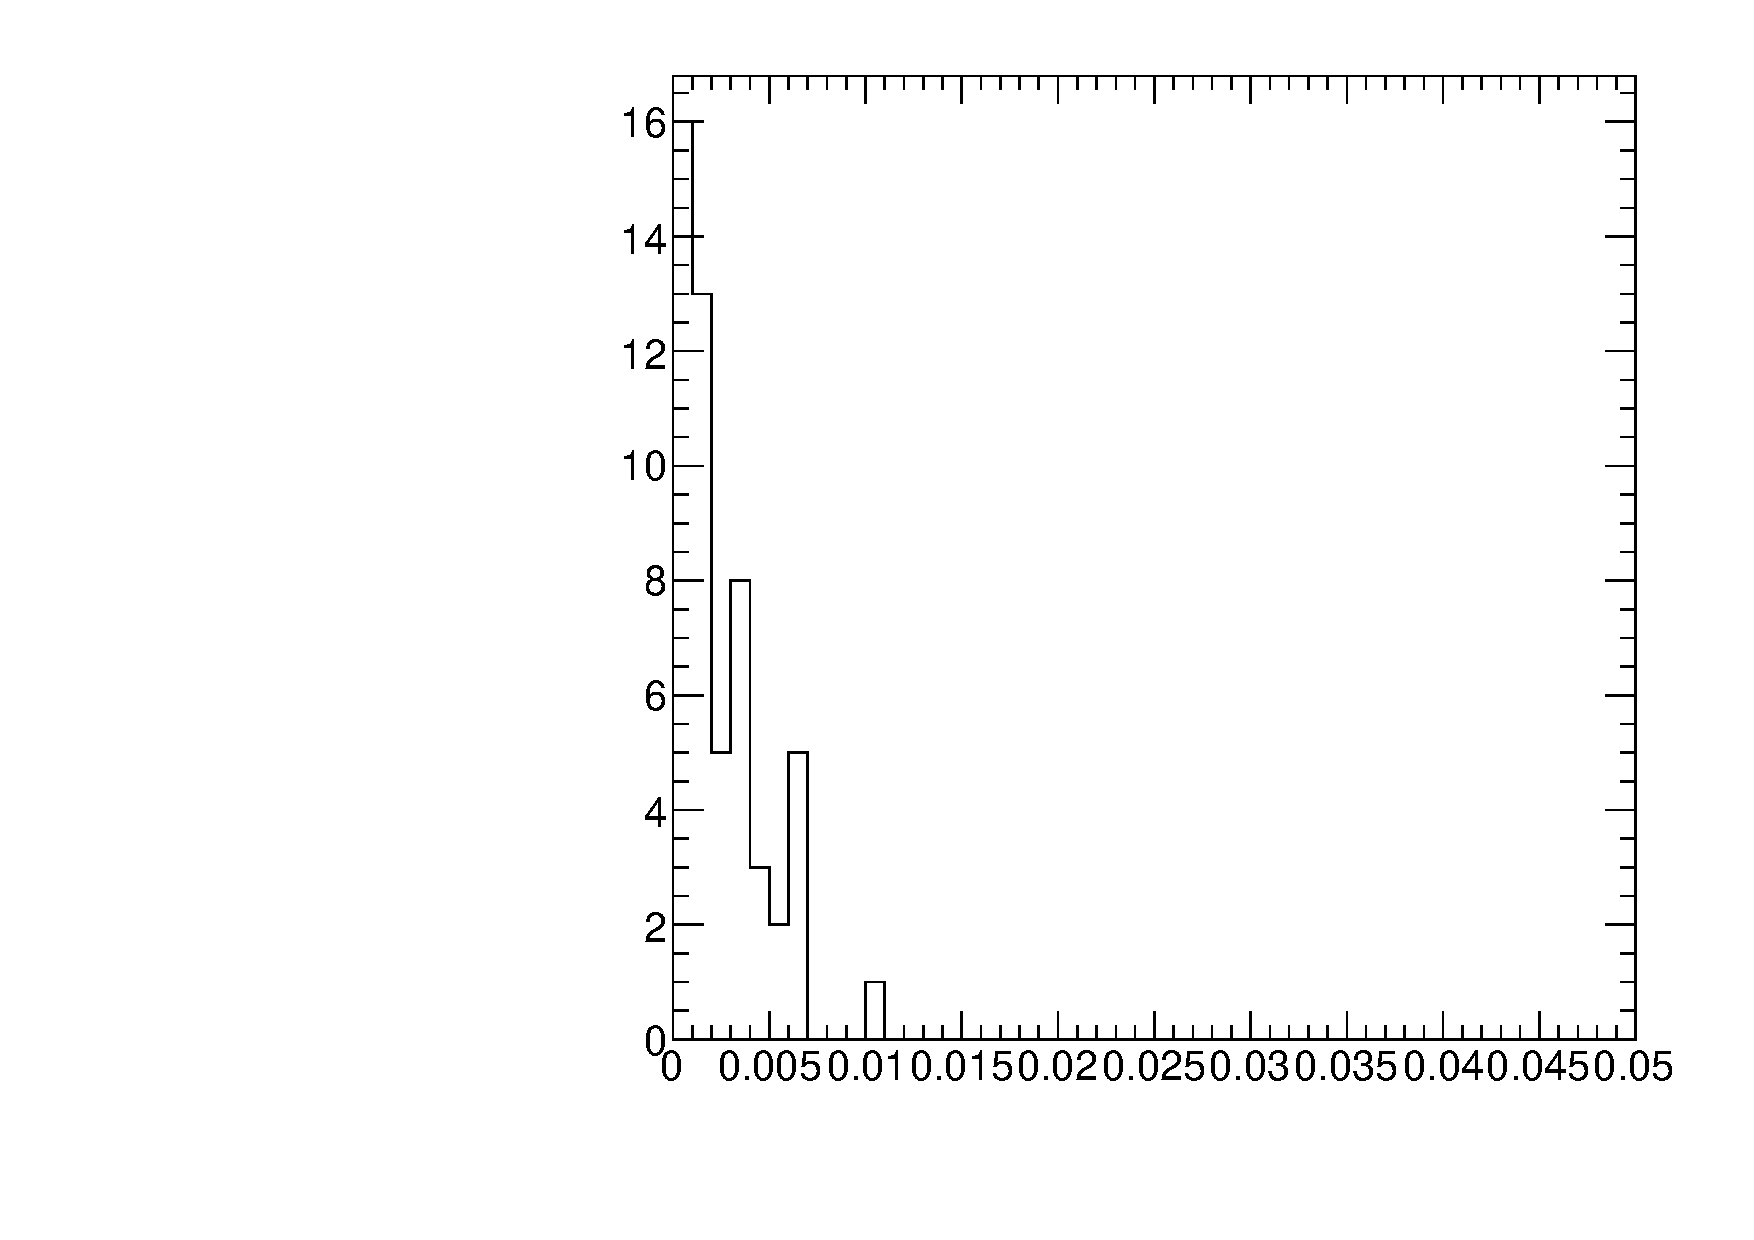
\includegraphics[width=0.3\textwidth]{Figures/AfterBDTCut_maxdoca_EndcapsUnblinded.pdf}
  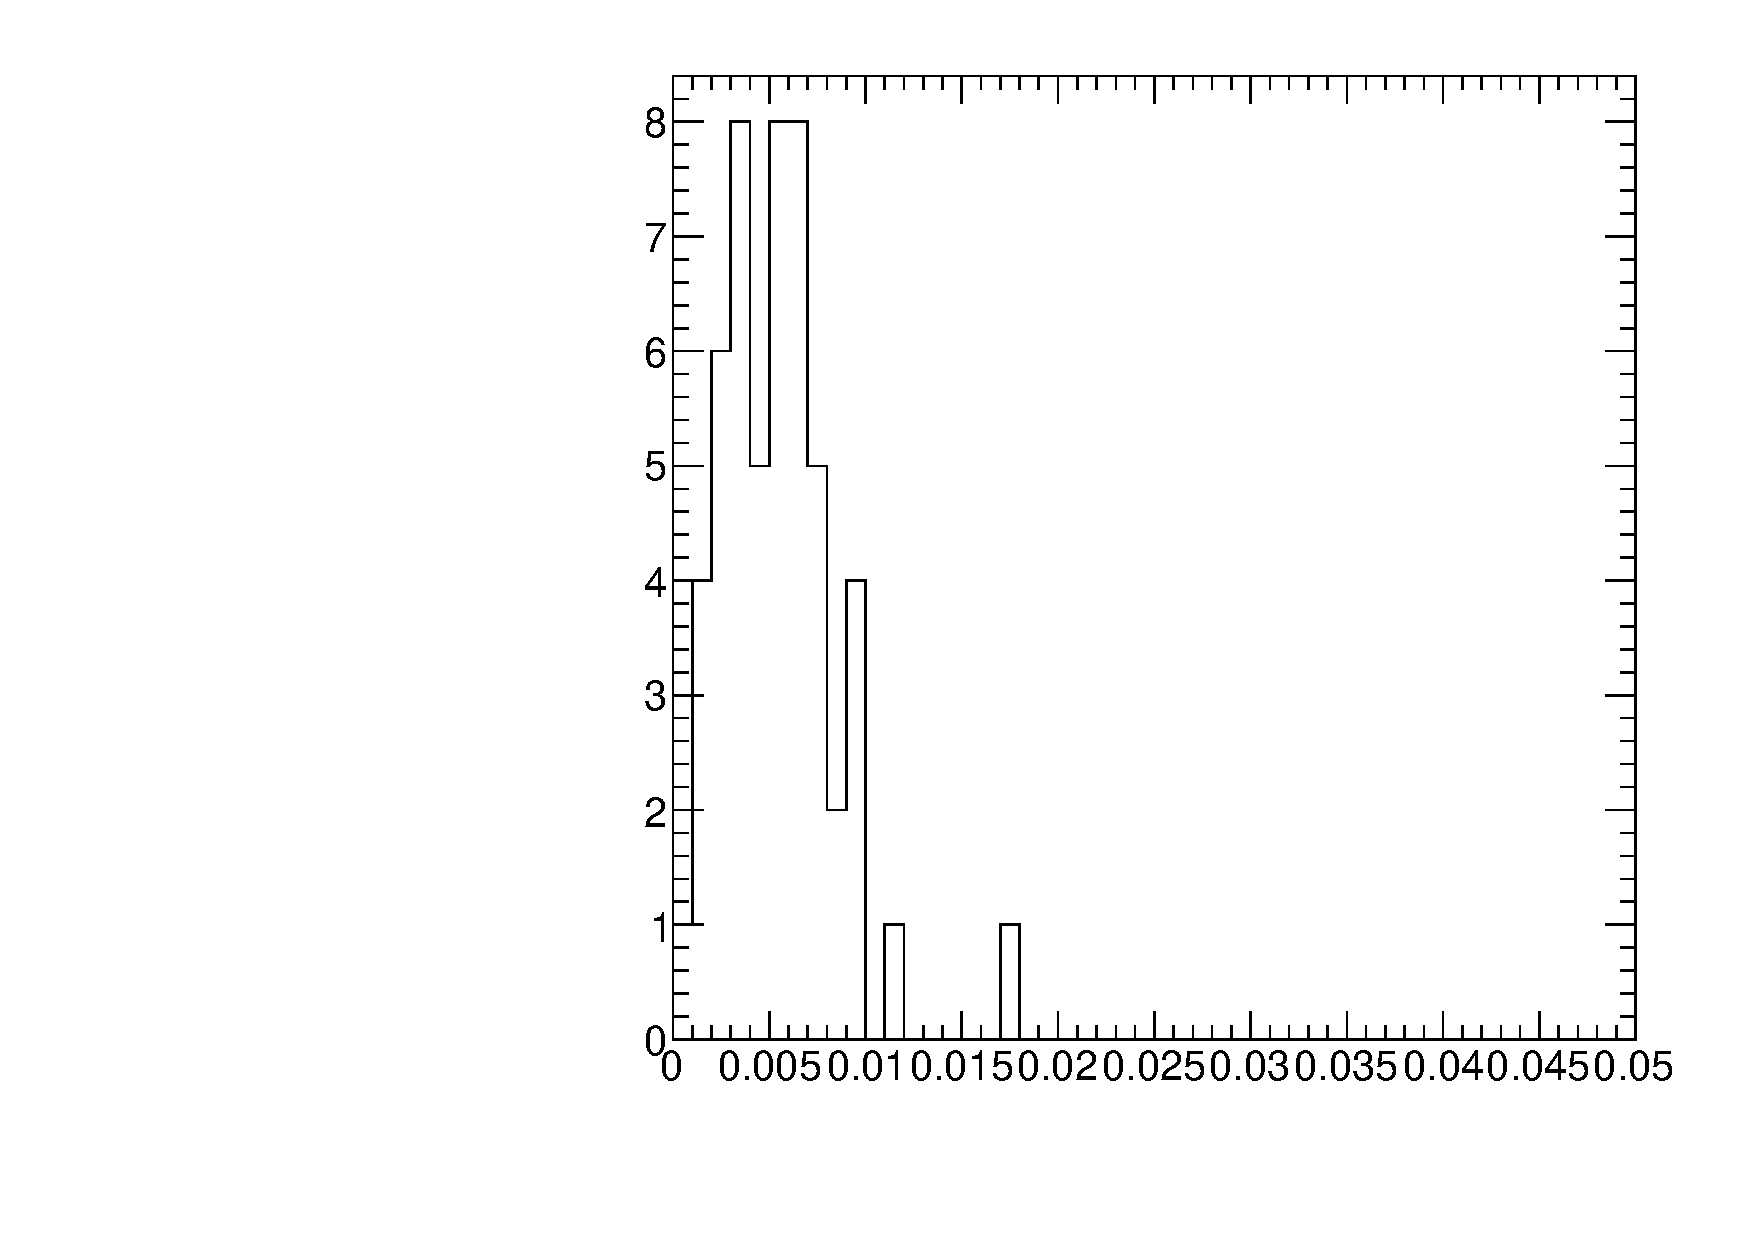
\includegraphics[width=0.3\textwidth]{Figures/AfterBDTCut_pvip_EndcapsUnblinded.pdf}
  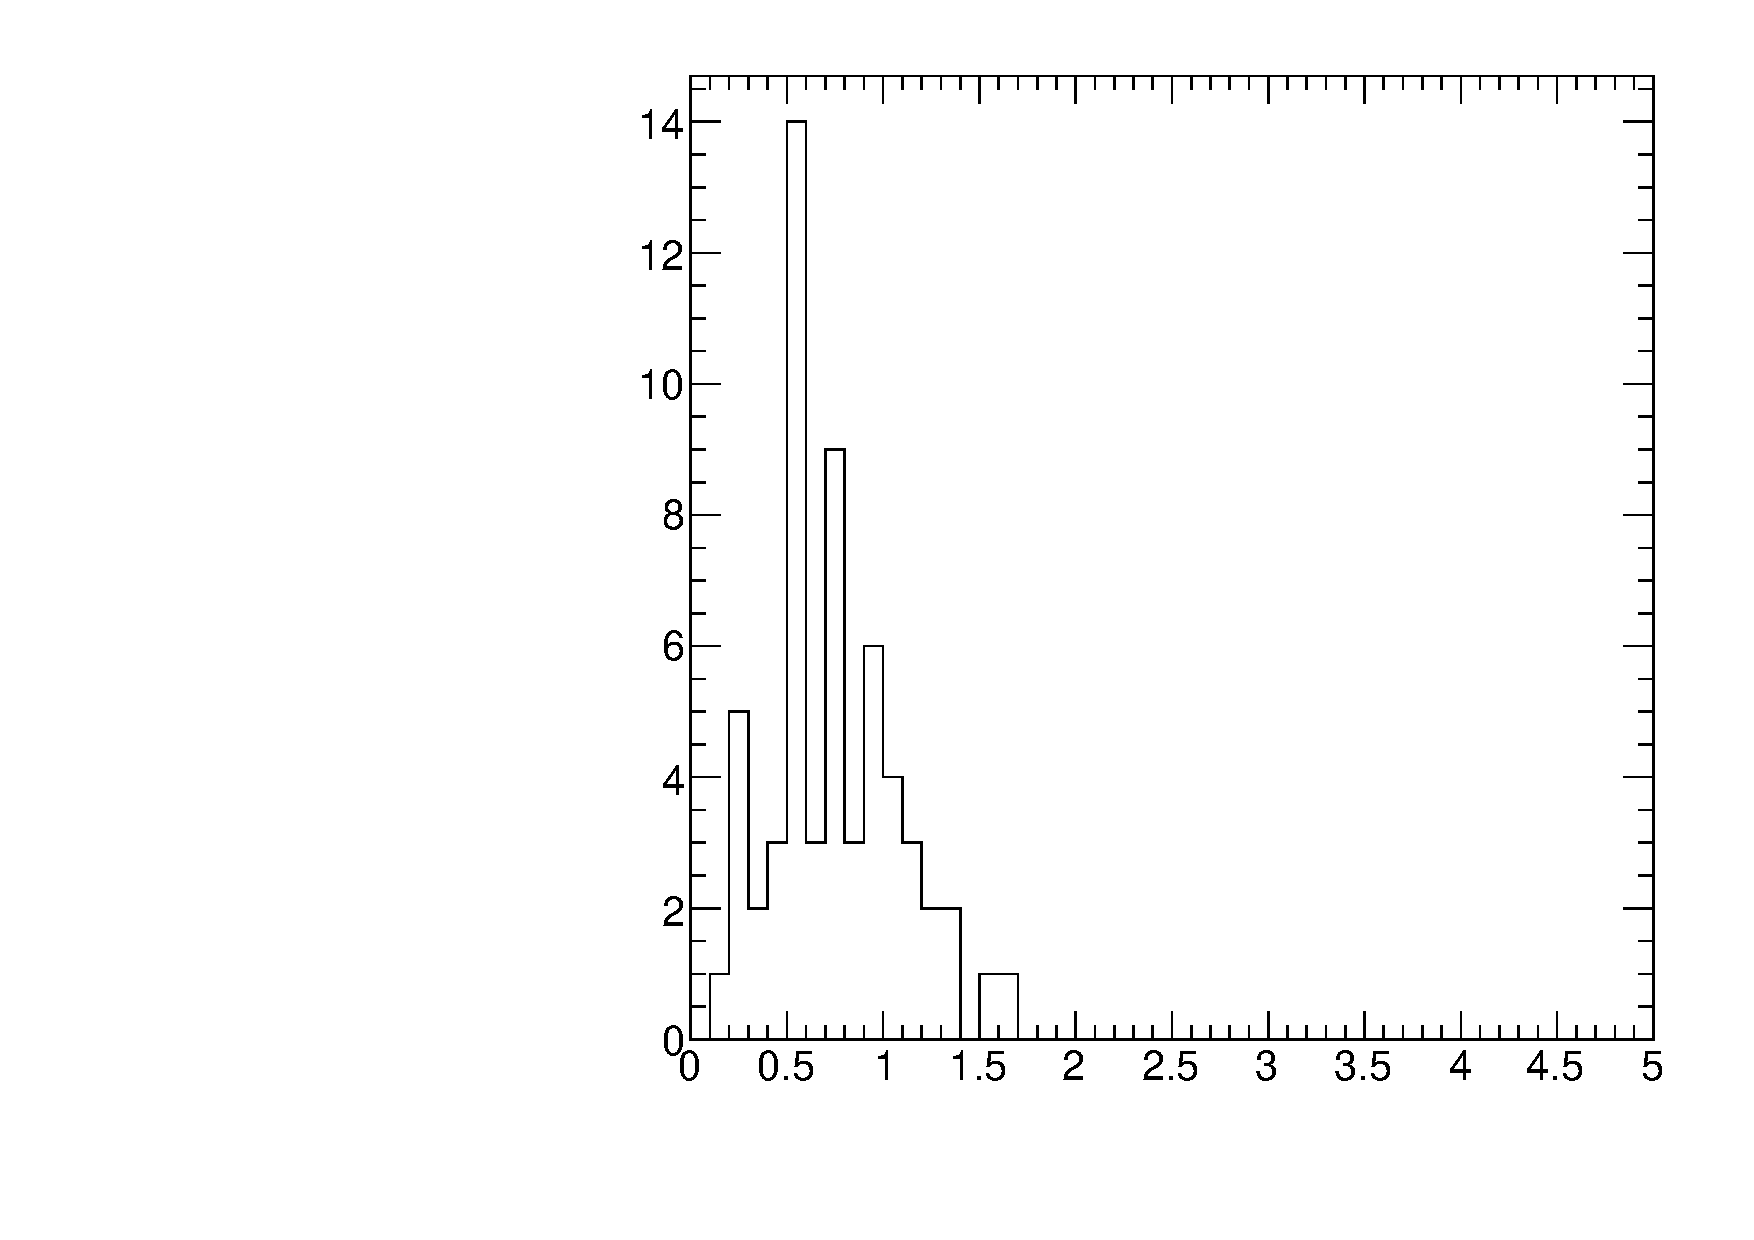
\includegraphics[width=0.3\textwidth]{Figures/AfterBDTCut_pvips_EndcapsUnblinded.pdf}
  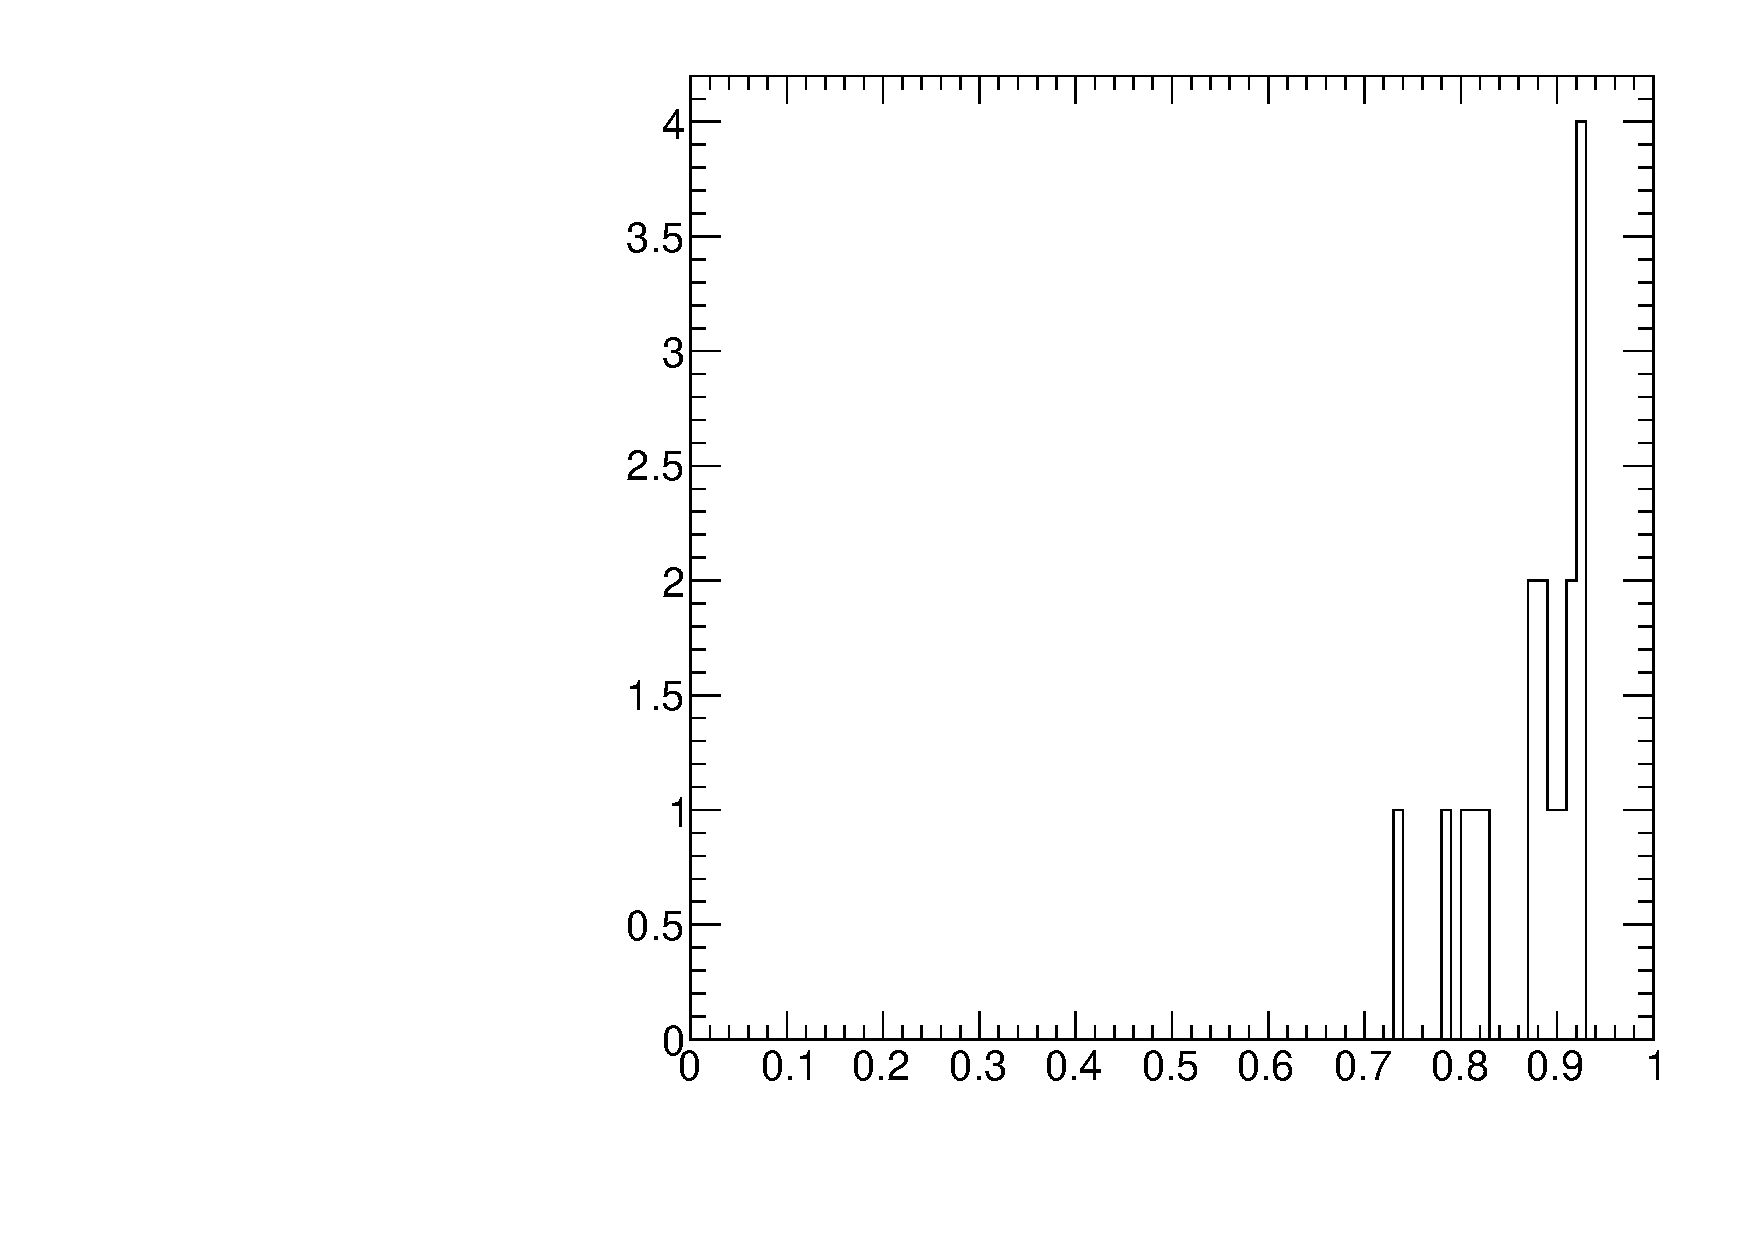
\includegraphics[width=0.3\textwidth]{Figures/AfterBDTCut_iso_EndcapsUnblinded.pdf}
  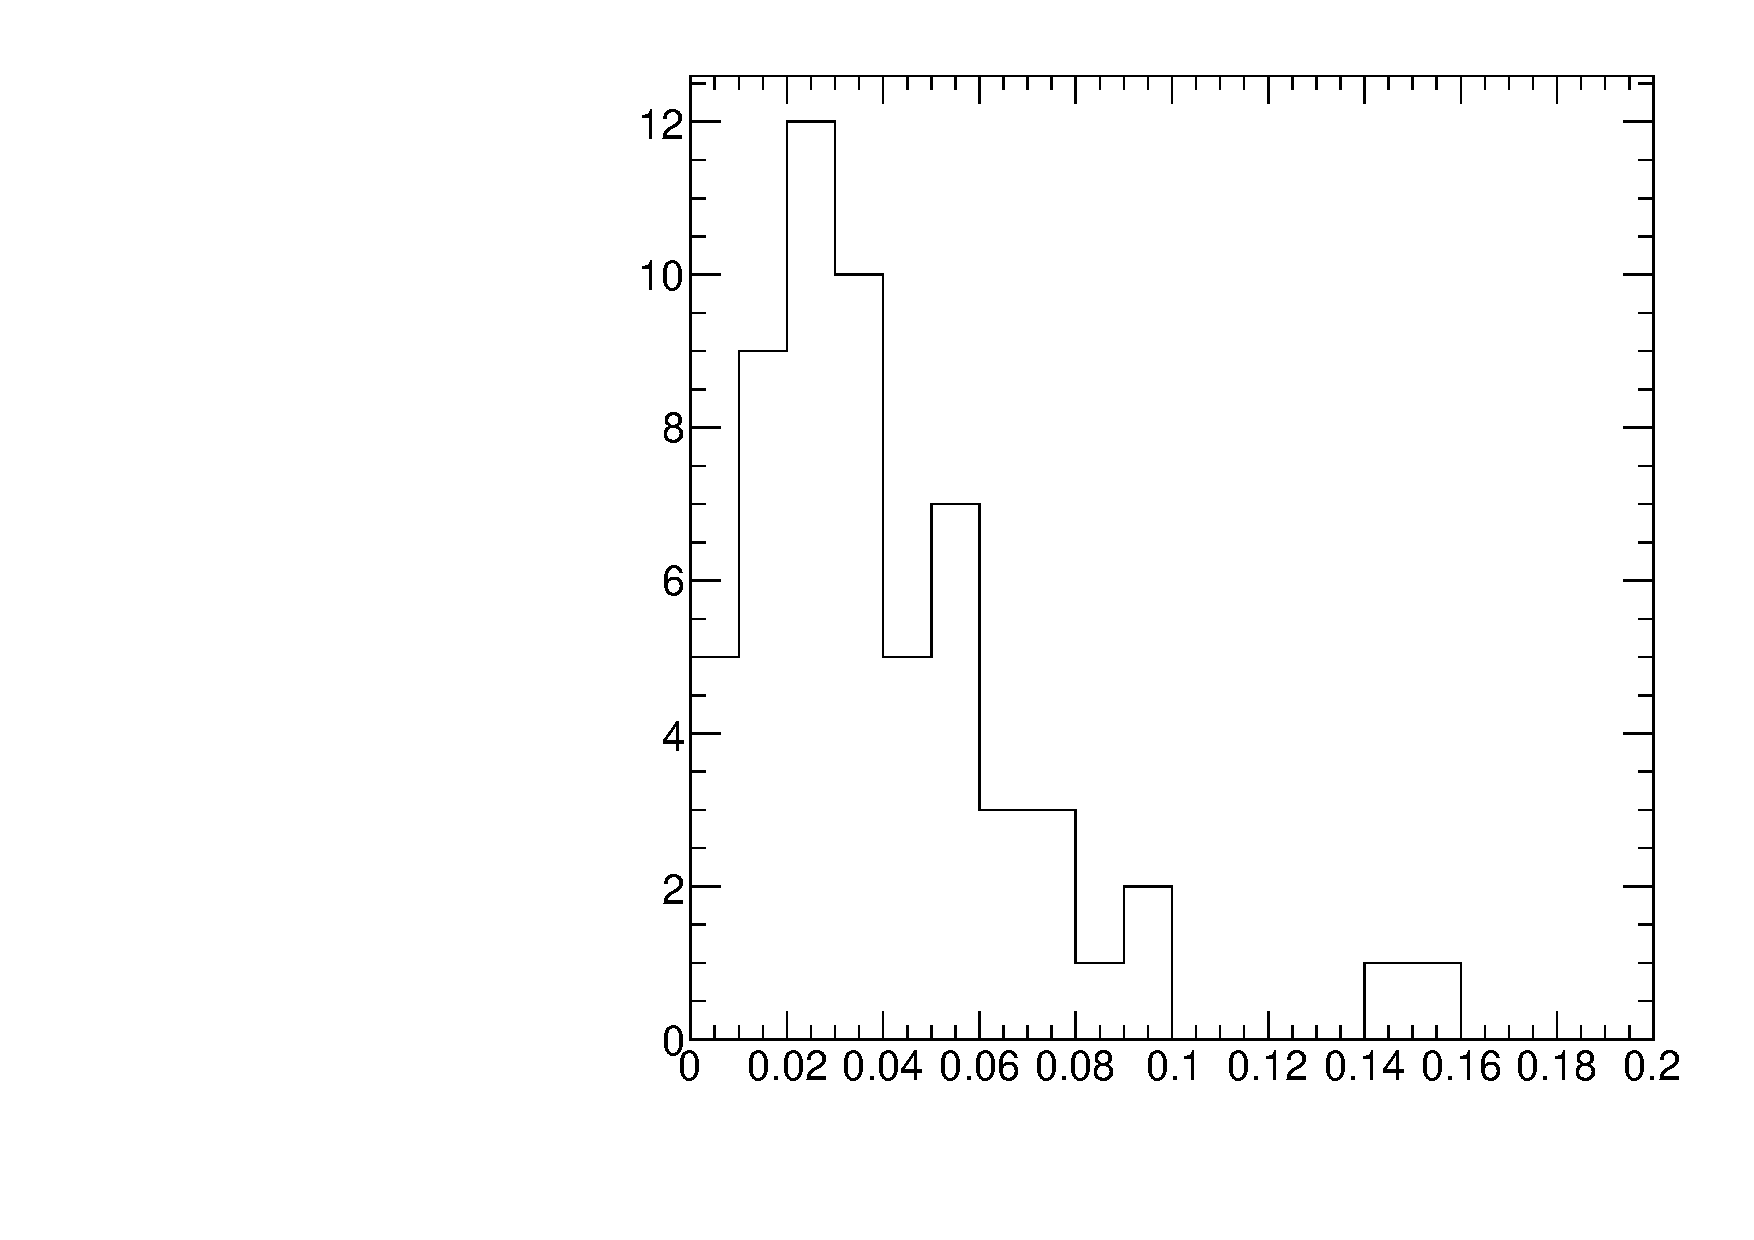
\includegraphics[width=0.3\textwidth]{Figures/AfterBDTCut_docatrk_EndcapsUnblinded.pdf}
  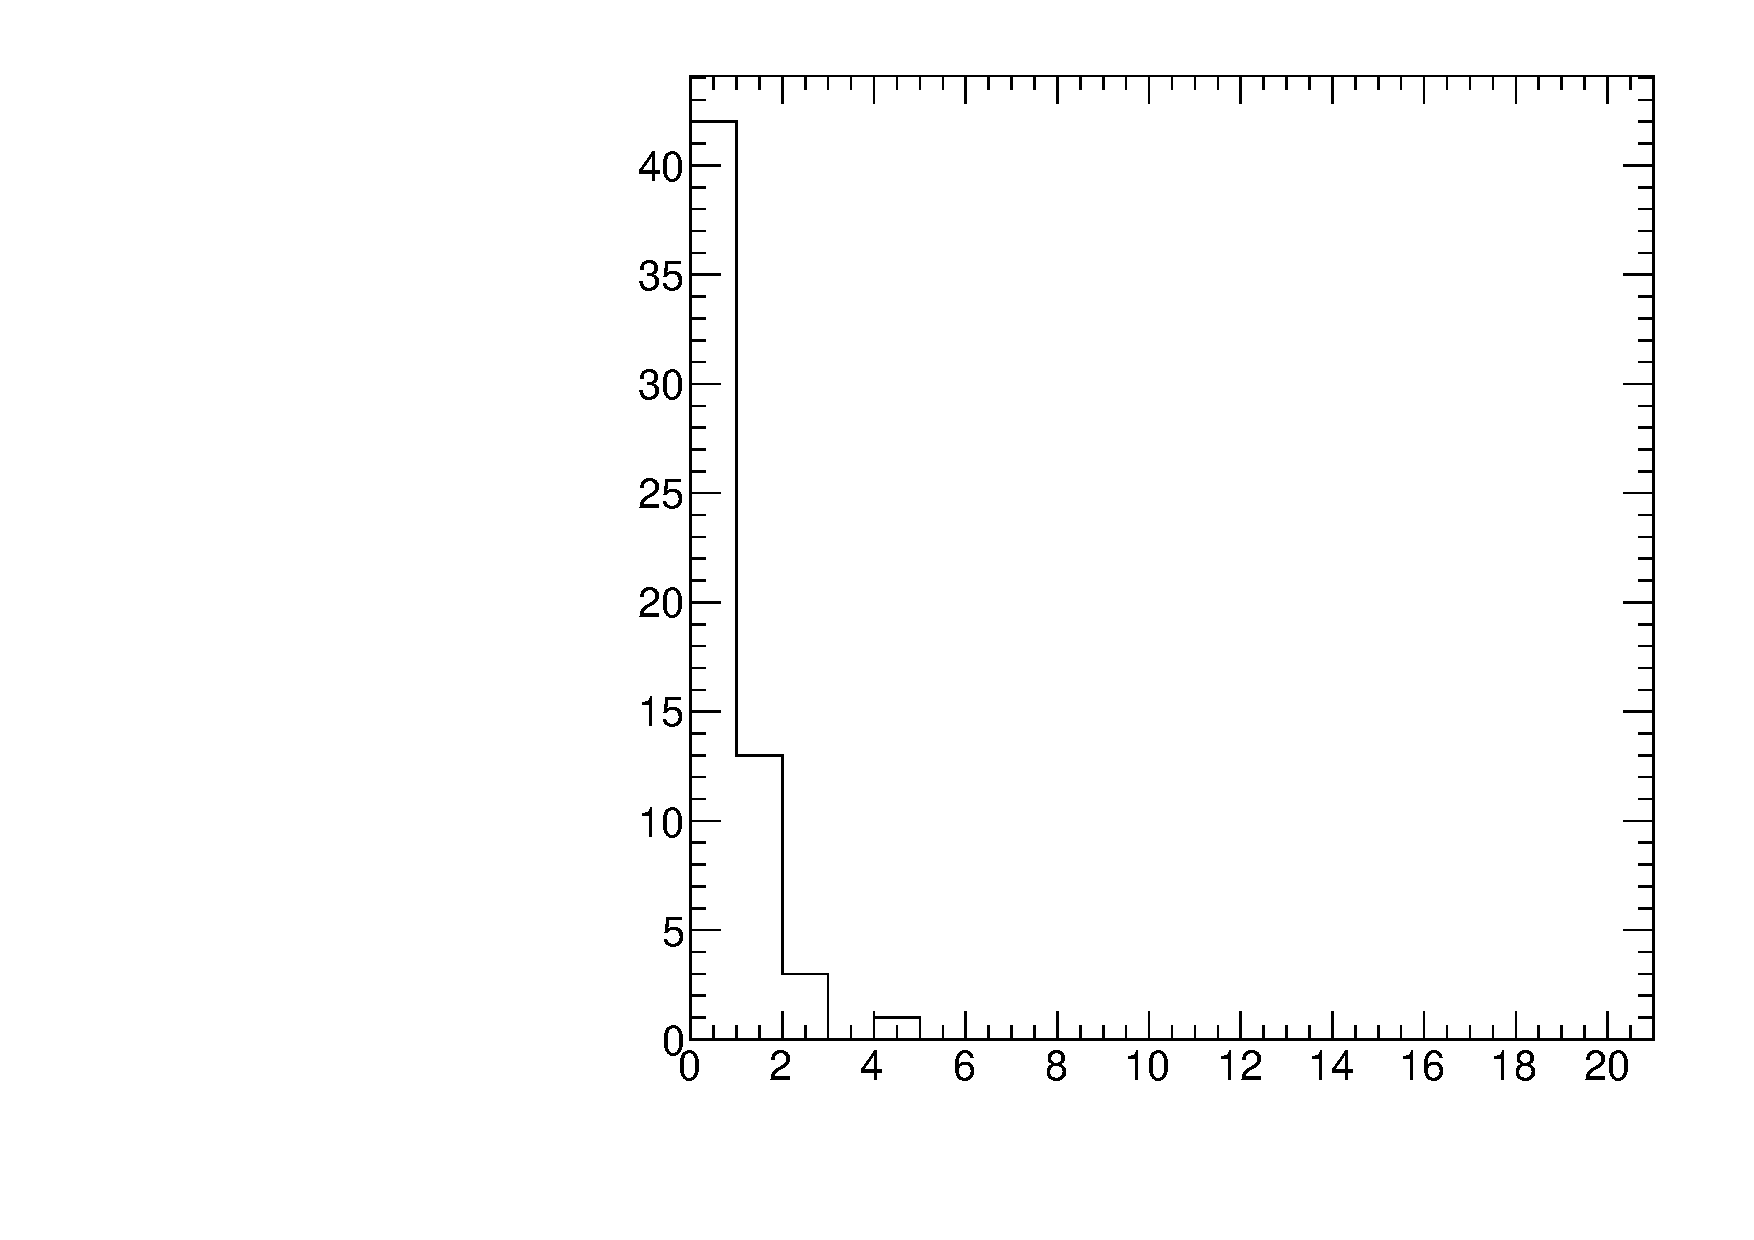
\includegraphics[width=0.3\textwidth]{Figures/AfterBDTCut_closetrk_EndcapsUnblinded.pdf}
  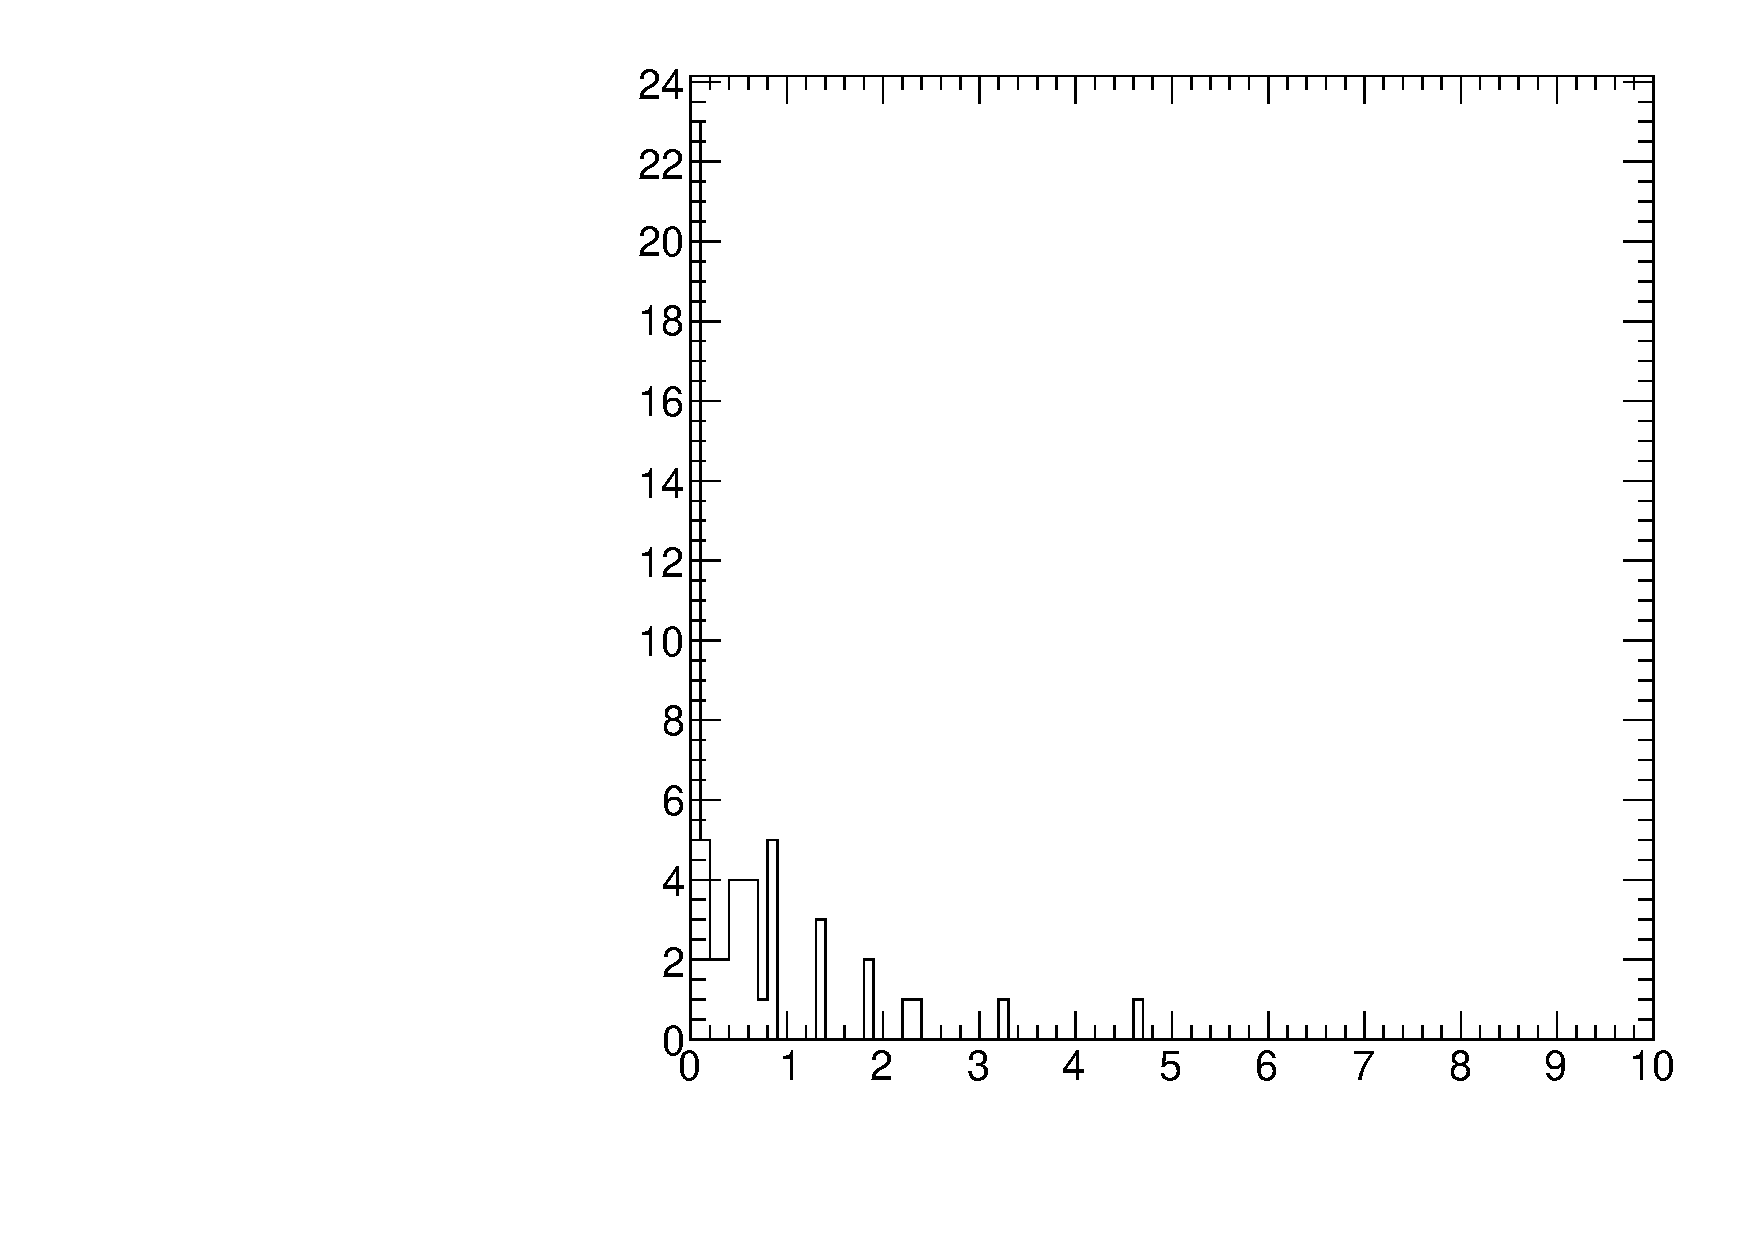
\includegraphics[width=0.3\textwidth]{Figures/AfterBDTCut_chi2dof_EndcapsUnblinded.pdf}
  \caption{Variable distributions for the endcaps after BDT cuts on unblinded data.}
  \label{fig:AfterBDTCutVariablesEndcapsUnblinded}
\end{figure}

In figure \ref{fig:overtrain_BDT_controlPlots} the standard control plots of TMVA with a linear scale are shown that check against overtraining of the BDT in the barrel and the endcap. 

\begin{figure}
        \centering
                \includegraphics[width=0.48\textwidth]{Figures/bdt/overtrain_BDT_barrel_0}
                \includegraphics[width=0.48\textwidth]{Figures/bdt/overtrain_BDT_endcaps_0}
                \includegraphics[width=0.48\textwidth]{Figures/bdt/overtrain_BDT_barrel_1}
                \includegraphics[width=0.48\textwidth]{Figures/bdt/overtrain_BDT_endcaps_1}
                \includegraphics[width=0.48\textwidth]{Figures/bdt/overtrain_BDT_barrel_2}
                \includegraphics[width=0.48\textwidth]{Figures/bdt/overtrain_BDT_endcaps_2}
        \caption{TMVA overtraining control plot for the barrel(left) and the endcap(right), for events of type 0...2 from the top to the bottom.}
        \label{fig:overtrain_BDT_controlPlots}
\end{figure}


Figures \ref{fig:applicationBDTOutputBarrel} and \ref{fig:applicationBDTOutputEndcaps} show the output of the BDT application on different samples for data and \BsMuMu simulation.

\begin{figure}
  \centering
  \includegraphics[width=0.45\textwidth]{Figures/ApplicationBDTOutput_Barrel.pdf}
  \includegraphics[width=0.45\textwidth]{Figures/ApplicationBDTOutput_Endcaps.pdf}
  \caption{BDT output distribution for the application on data for different control samples and the full sample for (left) and endcaps (right).}
  \label{fig:applicationBDTOutputBarrel}
\end{figure}

\begin{figure}
  \centering
  \includegraphics[width=0.45\textwidth]{Figures/ApplicationBDTOutput_BsMCBarrel.pdf}
  \includegraphics[width=0.45\textwidth]{Figures/ApplicationBDTOutput_BsMCEndcaps.pdf}
  \caption{BDT output distribution for the application on \BsMuMu signal MC different control samples and the full sample for (left) and endcaps (right).}
  \label{fig:applicationBDTOutputEndcaps}
\end{figure}


%%% [N] barrel
\begin{figure}
  \centering
  \includegraphics[width=0.45\textwidth]{Figures/bdt/BDT_barrel_roc}
  \includegraphics[width=0.45\textwidth]{Figures/bdt/BDT_barrel_eff} 
  \includegraphics[width=0.45\textwidth]{Figures/bdt/BDT_barrel_roc_zoom}
  \includegraphics[width=0.45\textwidth]{Figures/bdt/BDT_barrel_mass}
  \includegraphics[width=0.45\textwidth]{Figures/bdt/BDT_barrel_mass_unblind}
\caption{BDT barrel}
\end{figure}

\begin{figure}
  \centering
  \includegraphics[width=0.45\textwidth]{Figures/mlp/MLP_barrel_roc}
  \includegraphics[width=0.45\textwidth]{Figures/mlp/MLP_barrel_eff} 
  \includegraphics[width=0.45\textwidth]{Figures/mlp/MLP_barrel_roc_zoom}
  \includegraphics[width=0.45\textwidth]{Figures/mlp/MLP_barrel_mass}
  \includegraphics[width=0.45\textwidth]{Figures/mlp/MLP_barrel_mass_unblind}
\caption{MLP barrel}
\end{figure}


%%%
\begin{figure}
  \centering
  \includegraphics[width=0.45\textwidth]{Figures/bdt/BDT_endcaps_roc}
  \includegraphics[width=0.45\textwidth]{Figures/bdt/BDT_endcaps_eff} 
  \includegraphics[width=0.45\textwidth]{Figures/bdt/BDT_endcaps_roc_zoom}
  \includegraphics[width=0.45\textwidth]{Figures/bdt/BDT_endcaps_mass}
  \includegraphics[width=0.45\textwidth]{Figures/bdt/BDT_endcaps_mass_unblind}
\caption{BDT endcaps}
\end{figure}

\begin{figure}
  \centering
 \includegraphics[width=0.45\textwidth]{Figures/mlp/MLP_endcaps_roc}
  \includegraphics[width=0.45\textwidth]{Figures/mlp/MLP_endcaps_eff}
  \includegraphics[width=0.45\textwidth]{Figures/mlp/MLP_endcaps_roc_zoom}
  \includegraphics[width=0.45\textwidth]{Figures/mlp/MLP_endcaps_mass}
  \includegraphics[width=0.45\textwidth]{Figures/mlp/MLP_endcaps_mass_unblind}
\caption{MLP endcaps}
\end{figure}
